\documentclass[9pt]{article}
\usepackage[english]{babel}
\usepackage{amsmath,amsthm}
\usepackage{amsfonts}
\usepackage{graphicx}
\usepackage[margin=0.2in]{geometry}
\newcommand{\setlinespacing}[1]{\setlength{\baselineskip}{#1 \defbaselineskip}}
\newcommand{\doublespacing}{\setlength{\baselineskip}{2.0 \defbaselineskip}}
\newcommand{\singlespacing}{\setlength{\baselineskip}{\defbaselineskip}}
\newcommand{\A}{{\cal A}}
\newcommand{\h}{{\cal H}}
\newcommand{\s}{{\cal S}}
\newcommand{\W}{{\cal W}}
\newcommand{\BH}{\mathbf B(\cal H)}
\newcommand{\KH}{\cal  K(\cal H)}
\newcommand{\Real}{\mathbb R}
\newcommand{\Complex}{\mathbb C}
\newcommand{\Field}{\mathbb F}
\newcommand{\RPlus}{[0,\infty)}
\newcommand{\norm}[1]{\left\Vert#1\right\Vert}
\newcommand{\essnorm}[1]{\norm{#1}_{\text{\rm\normalshape ess}}}
\newcommand{\abs}[1]{\left\vert#1\right\vert}
\newcommand{\set}[1]{\left\{#1\right\}}
\newcommand{\seq}[1]{\left<#1\right>}
\newcommand{\eps}{\varepsilon}
\newcommand{\To}{\longrightarrow}
\newcommand{\RE}{\operatorname{Re}}
\newcommand{\IM}{\operatorname{Im}}
\newcommand{\Poly}{{\cal{P}}(E)}
\newcommand{\EssD}{{\cal{D}}}
\newcommand{\field}[1]{\mathbb{#1}}
\newcommand{\C}{\field{C}}
\newcommand{\R}{\field{R}}
\newcommand{\script}[1]{\mathcal{#1}}
\newcommand{\fall}{\; \forall \;}
\newcommand{\exts}{\; \exists \;}
\newcommand{\mbf}[1]{\mathbf{#1}}
\newcommand{\binomial}[2]{\biggl( \begin{array}{c}  #1 \\ #2  \\ \end{array} \biggr) }
\newcommand{\fderiv}[2]{ \frac{d}{ d #1} \: #2}
\newcommand{\sderiv}[2]{ \frac{d^2}{ d^2 #1} \: #2}
\newcommand{\pfderiv}[2]{ \frac{\partial}{ \partial #1} \: #2}
\newcommand{\psderiv}[2]{ \frac{\partial^2}{ \partial^2 #1} \: #2}
\newcommand{\mat}[1]{\mathbf{#1}}
\DeclareSymbolFont{AMSb}{U}{msb}{m}{n}
\DeclareMathSymbol{\dblz}{\mathalpha}{AMSb}{"5A}
\DeclareMathSymbol{\dblr}{\mathalpha}{AMSb}{"52}
\DeclareMathSymbol{\dblt}{\mathalpha}{AMSb}{"54}
\DeclareMathSymbol{\dblq}{\mathalpha}{AMSb}{"51}
\DeclareMathSymbol{\dbln}{\mathalpha}{AMSb}{"4E}
\DeclareMathSymbol{\dblf}{\mathalpha}{AMSb}{"46}
\DeclareMathSymbol{\dblc}{\mathalpha}{AMSb}{"43}
\DeclareMathSymbol{\dbld}{\mathalpha}{AMSb}{"44}
\theoremstyle{plain}
\newtheorem{thm}{Theorem}[section]
\newtheorem{cor}[thm]{Corollary}
\newtheorem{lem}[thm]{Lemma}
\newtheorem{prop}[thm]{Proposition}
\theoremstyle{definition}
\newtheorem{defn}{Definition}[section]
\theoremstyle{remark}
\newtheorem{rem}{Remark}[section]
\numberwithin{equation}{section}
\renewcommand{\theequation}{\thesection.\arabic{equation}}
\begin{document}
\title{Regression of KL Software Distribution   }
\author{KL Software Libraries}
\date{Wed Jun 11 17:19:39 2014
}
\maketitle
\textbf{ KL Library test output.  This LaTex file and the associated diagrams are produced by the KL software libraries.}
\subsubsection{Matrix Quick Check <double>}
QueryPerformanceCounter  =  0.0950287
\subsubsection{Linear Regression atan data 3x1}
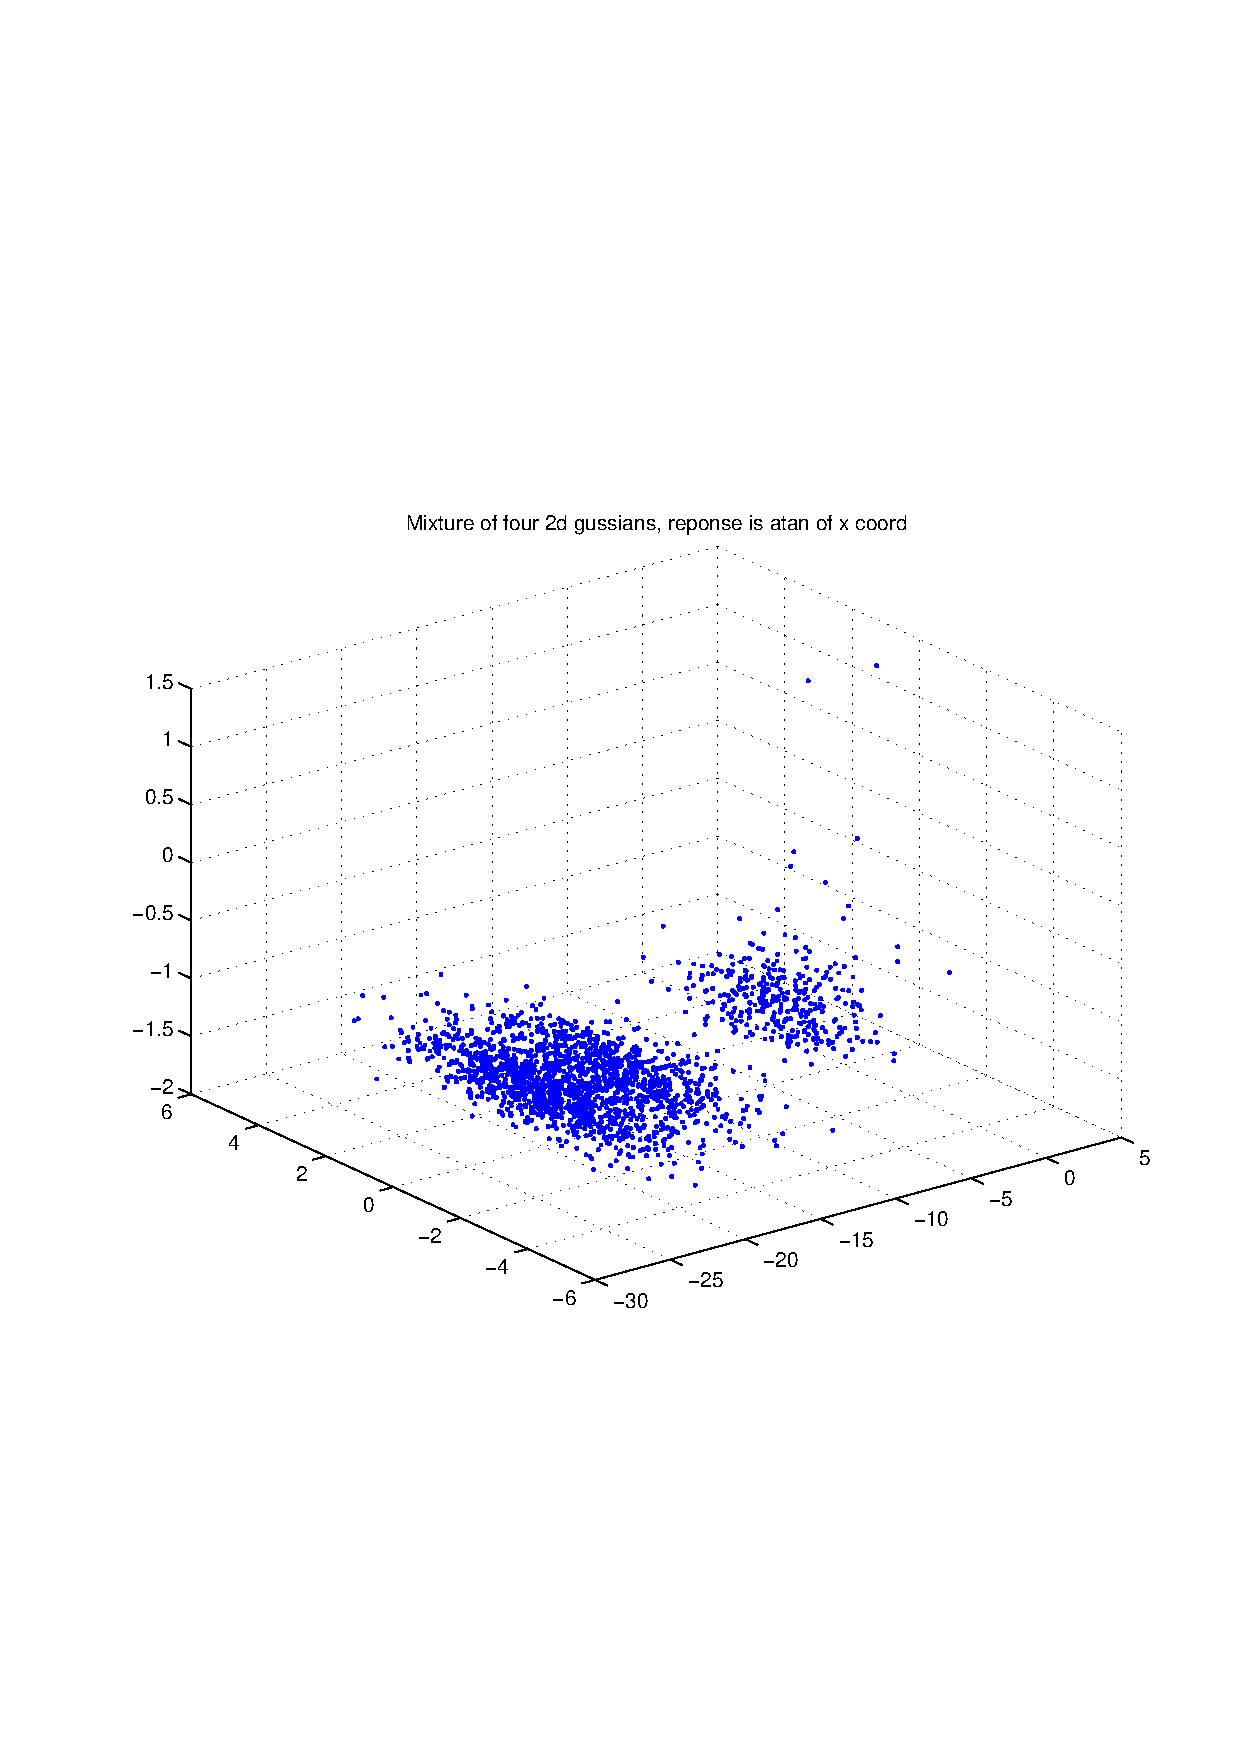
\includegraphics[width=10.0cm,height=10.0cm]{AtanDataSet.pdf}

\subsubsection{3 x 1 Linear Regression}
Sample size = 4000

Number of features = 3

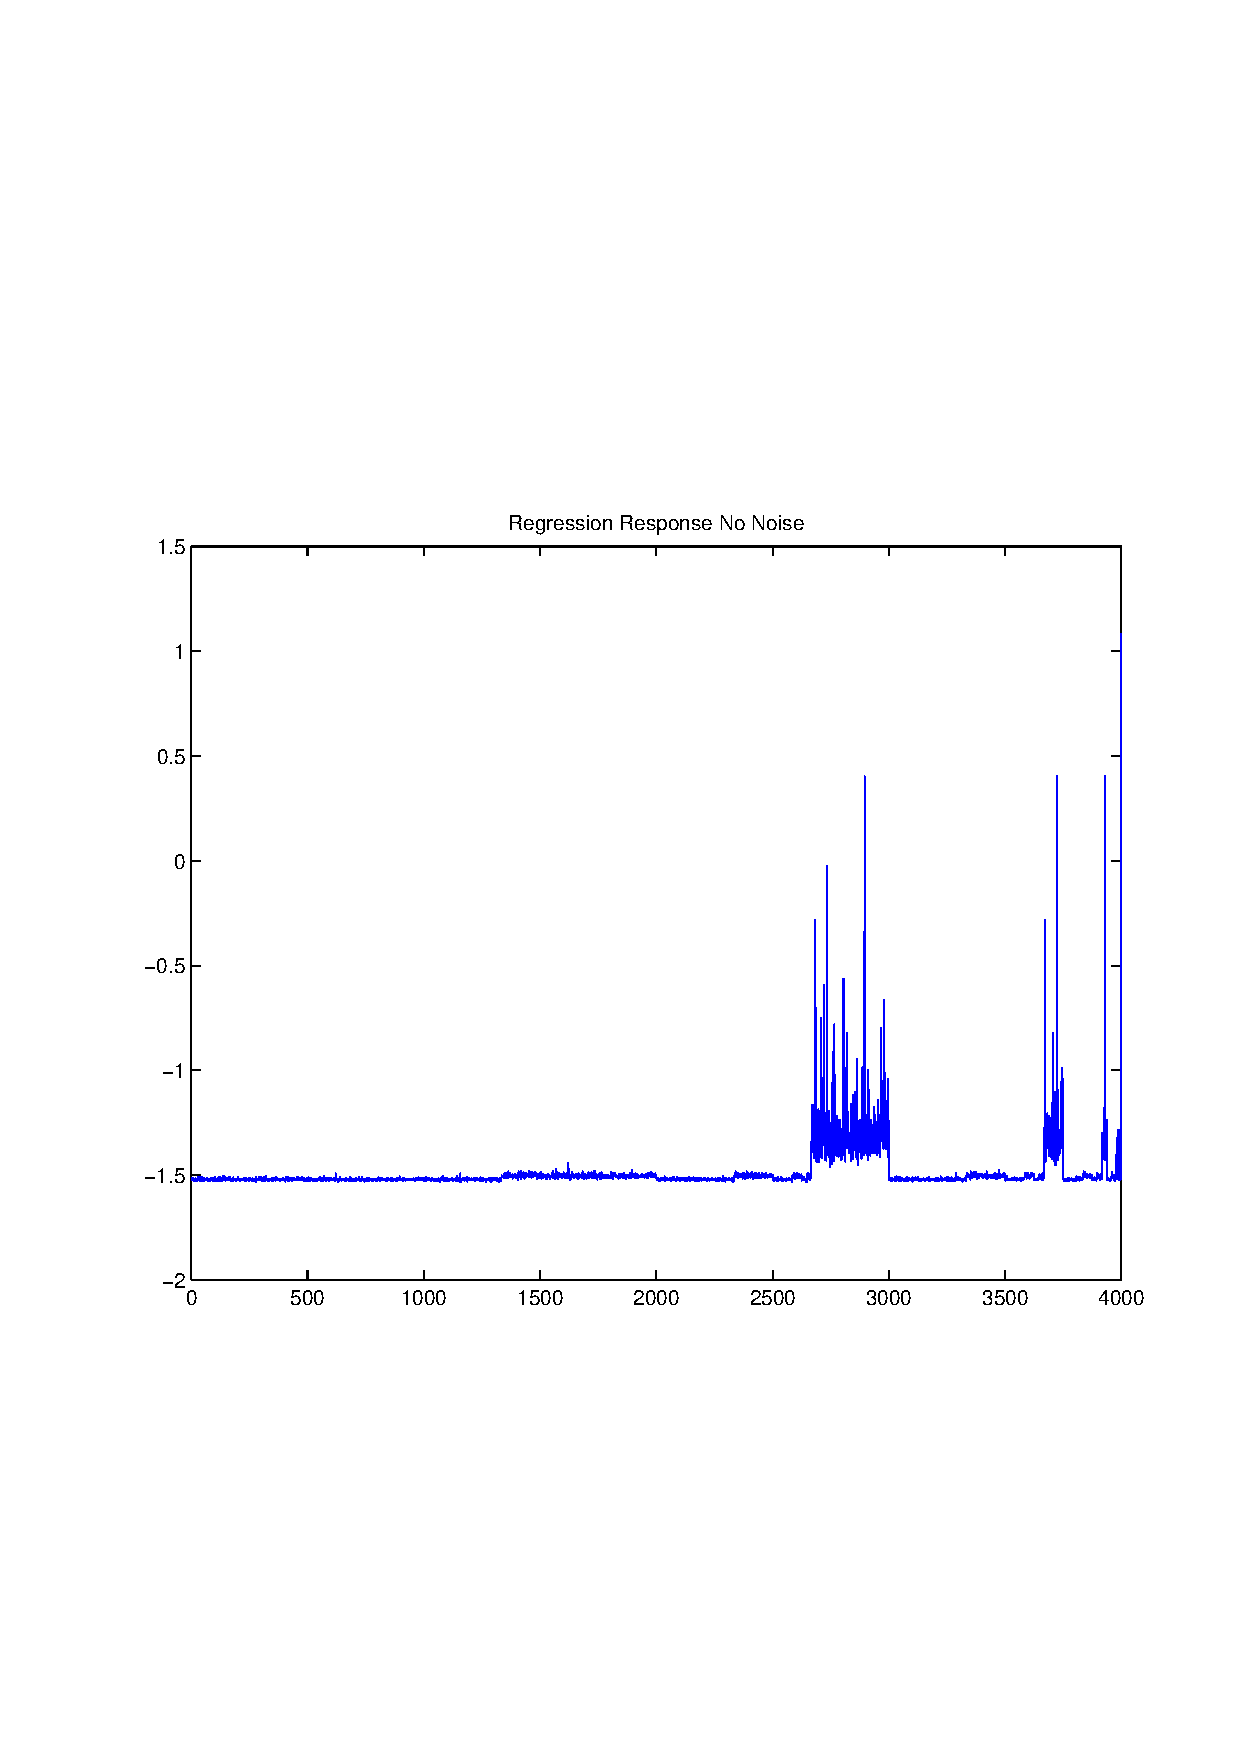
\includegraphics[width=10.0cm,height=10.0cm]{AtanDataSet_regression_response_no_noise.pdf}

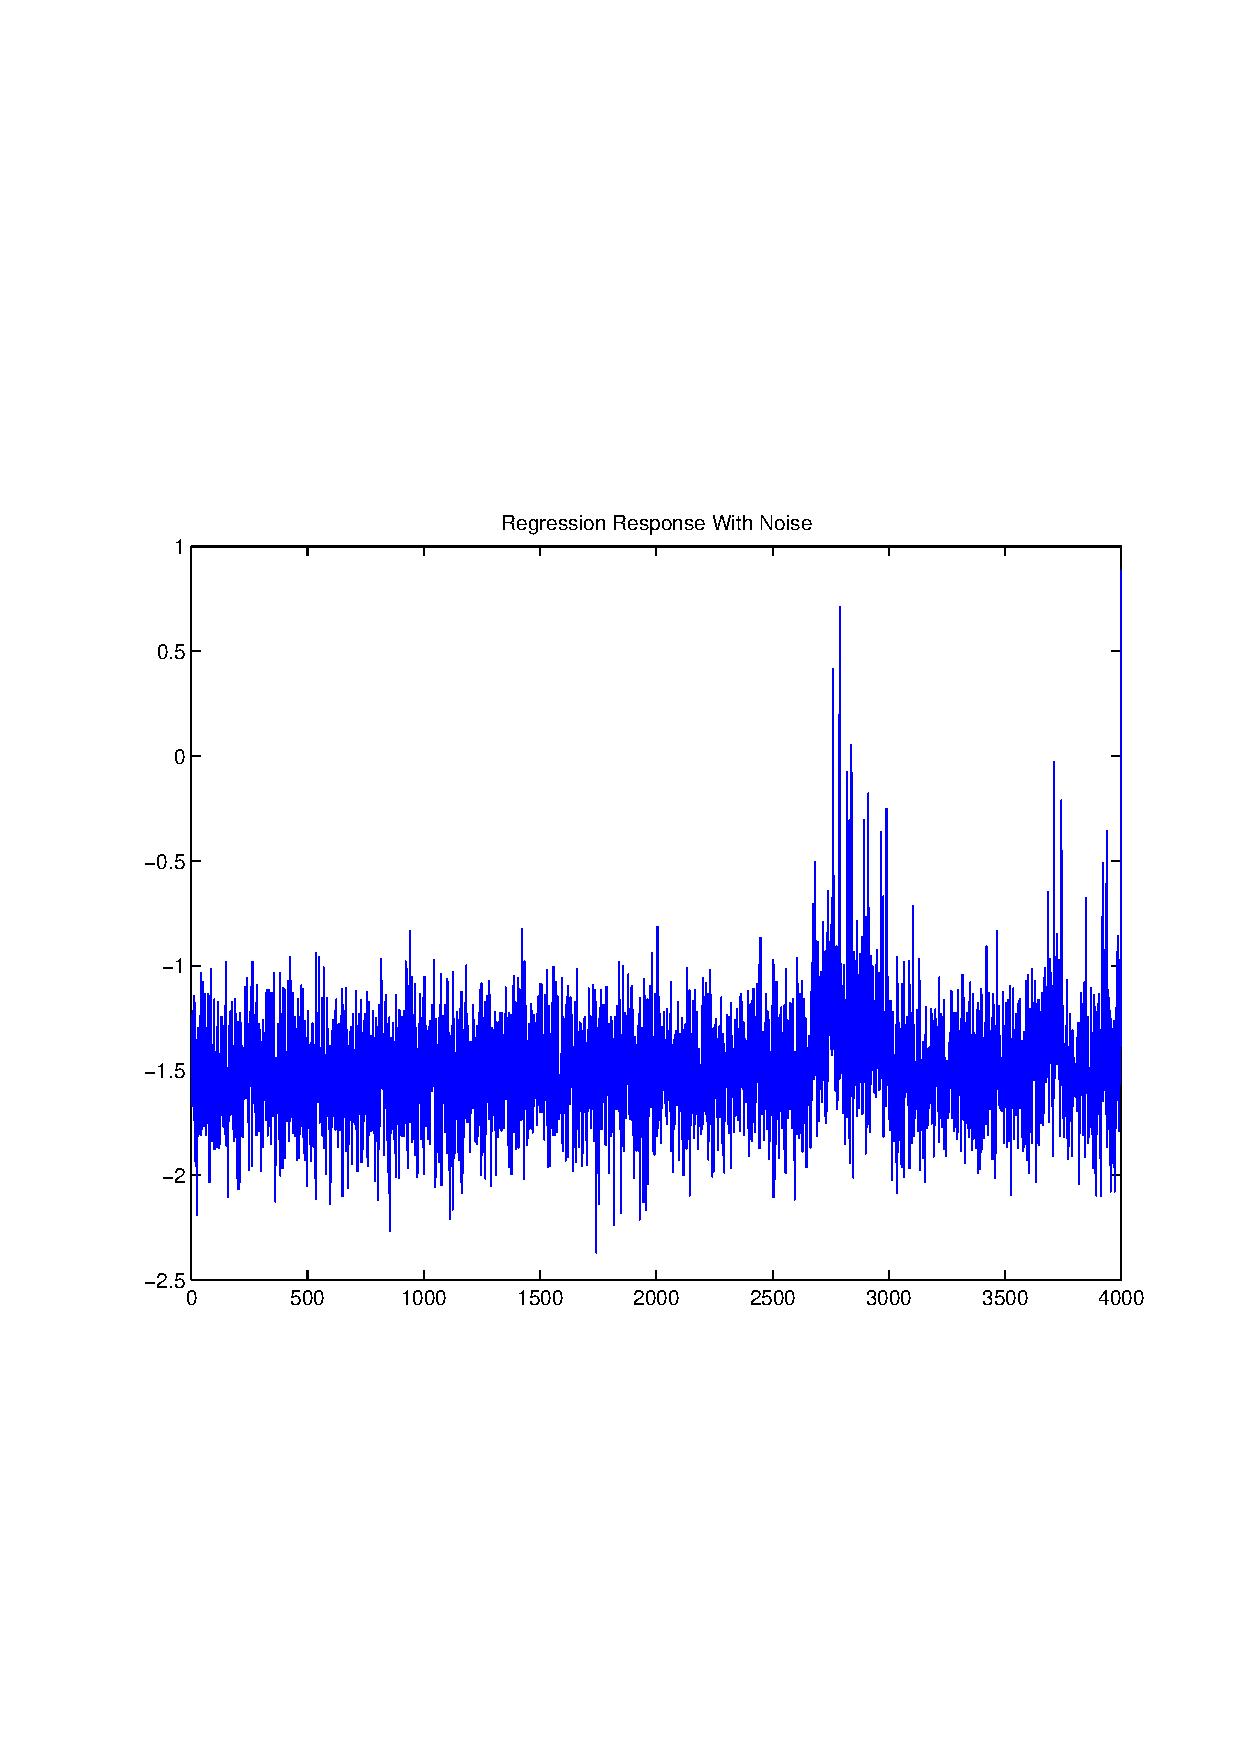
\includegraphics[width=10.0cm,height=10.0cm]{AtanDataSet_regression_response_with_noise.pdf}

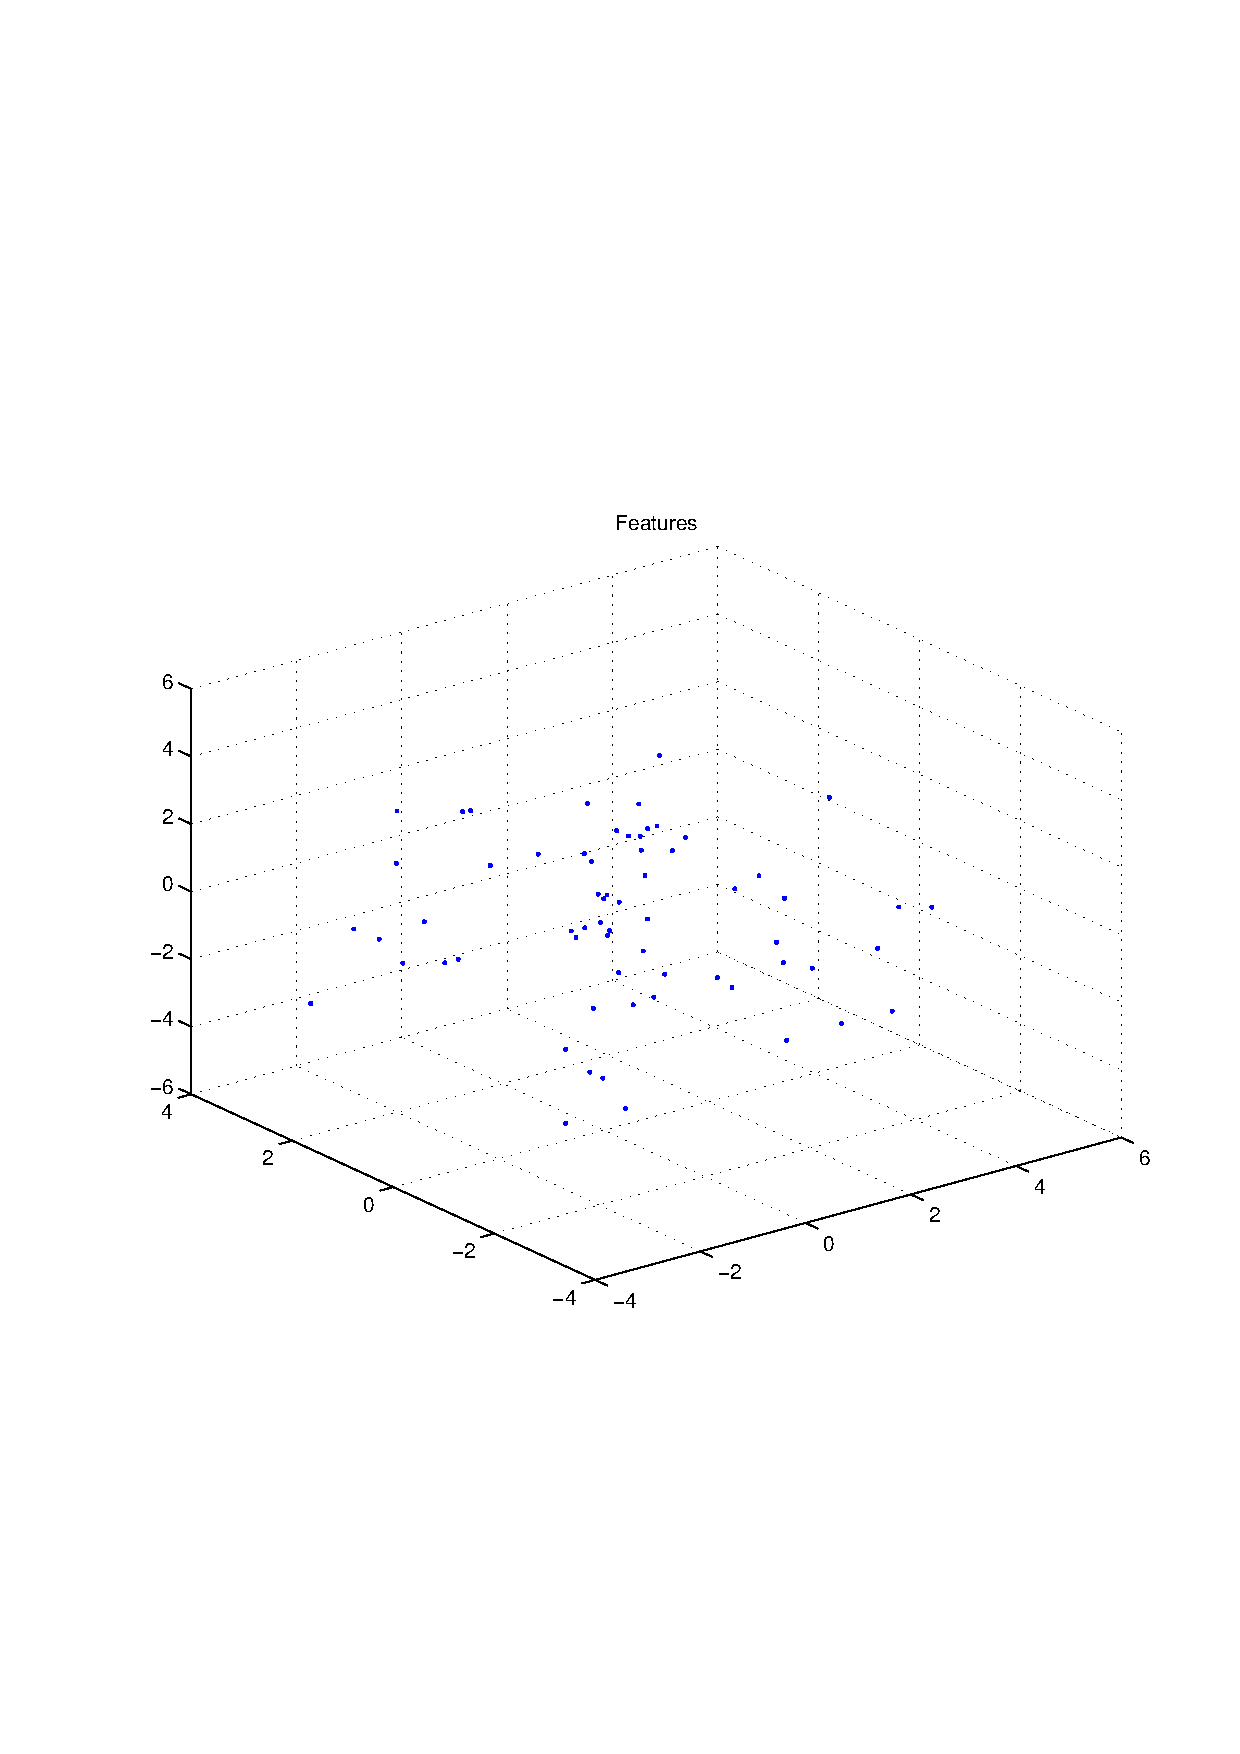
\includegraphics[width=10.0cm,height=10.0cm]{regression_features.pdf}

Response
-1.43751
-1.65688
-1.39825
1.5997
-1.31279
-1.33175
-1.20411
1.56964
-1.32116
-1.14059
-1.57179
1.18508
-1.74261
-1.48858
-1.2303
0.914332
-1.17288
-1.36061
-1.72804
1.26739
-1.42564
-1.5198
-1.10402
1.01455
-1.48005
-2.1775
-1.15506
1.38505
-1.45644
-1.7538
-1.36058
1.51512
-1.80722
-1.77617
-1.50621
1.59033
-1.26129
-1.48465
-1.11831
1.06231
-1.15856
-1.35128
-0.333051
1.67526
-1.23094
-1.76046
-1.33806
1.14311
-1.52531
-1.06838
-1.24732
1.52573
-1.55117
-1.73224
-0.931009
1.25341
-1.4541
-1.11898
-1.44504
1.1891
-1.48973
-1.75606
-1.2837
1.23338
-1.7981
-1.26224
-0.492669
1.23863
-1.52955
-1.46754
-0.677743
1.79312
-1.74412
-1.22155
-1.52265
0.948098
-1.60624
-2.00848
-0.930768
1.26798
-1.44128
-1.51534
-1.48979
1.7851
-1.34083
-0.986731
-1.2006
1.41713
-1.84887
-1.53978
-1.23524
1.50193
-1.38046
-1.50296
-1.02944
1.3218
-1.38195
-1.21406
-0.95427
0.983682
-1.83191
-1.52173
-1.49725
0.886347
-1.70209
-1.81831
-1.23557
1.33258
-1.61186
-1.61095
-1.64145
1.42713
-1.18297
-1.36819
-1.65033
1.04876
-1.81259
-1.40164
-1.65966
1.3097
-1.66789
-1.60147
-1.51072
1.172
-1.80699
-1.54655
-1.57419
1.3133
-1.41894
-1.2376
-1.57918
0.993327
-1.69779
-1.64196
-1.24075
1.37719
-1.5763
-1.75209
-1.48115
1.45831
-1.66255
-1.43786
-0.914512
1.14076
-1.79079
-1.15648
-1.16775
1.94486
-1.62209
-1.74541
-1.27252
1.39615
-1.47512
-1.69403
-0.52451
1.30318
-1.68057
-1.4739
-1.9532
1.0975
-1.37818
-1.27295
-0.524462
1.50751
-1.6791
-1.5686
-0.907642
1.69532
-1.72008
-1.49028
-1.24261
1.28985
-1.36968
-1.16492
-0.891302
1.36288
-1.63817
-1.77335
-1.38935
1.24598
-1.50131
-1.5894
-1.76671
0.397456
-1.48142
-1.80501
-0.952158
1.63041
-1.55701
-1.43615
-1.57584
1.5939
-1.73398
-1.37162
-1.30321
1.40433
-2.01041
-1.39249
-1.31371
1.24775
-1.2602
-1.32739
-1.08117
1.19779
-1.33867
-1.37038
-1.04804
1.54575
-1.45983
-1.19676
-1.15549
1.6348
-1.60999
-1.71475
-0.994582
1.49728
-1.51448
-1.79893
-1.58466
1.26971
-1.82115
-1.42766
-1.51284
1.12704
-1.44724
-1.37666
-1.47262
1.27972
-1.54383
-1.08743
-1.32344
1.32454
-1.39018
-1.14855
-1.28343
1.27483
-1.52251
-1.43526
-1.32151
1.45156
-1.47439
-1.50649
-1.2319
1.28704
-1.33023
-1.7287
-1.14636
1.30898
-1.96927
-1.50575
-1.32355
1.40758
-1.42541
-1.33165
-0.442533
1.38426
-1.32814
-1.55065
-0.97124
0.960183
-1.9547
-1.44847
-0.438902
1.60336
-1.65593
-1.16566
-0.983336
1.67958
-1.55647
-1.59697
-0.493978
1.68504
-1.62612
-1.42054
-1.46912
1.42983
-1.18809
-1.71181
-0.657224
1.11871
-1.34867
-1.44719
-0.928398
1.00698
-1.64359
-1.58666
-1.55217
1.24126
-1.51843
-1.35283
-1.19596
0.800435
-1.44317
-1.29747
-1.45086
1.1936
-1.42072
-1.46821
-1.70298
0.915864
-1.37929
-1.44242
-1.41609
1.28122
-1.67996
-1.59659
-1.08518
0.965592
-1.45748
-1.73161
-1.154
1.37062
-1.64719
-1.32511
-1.47141
0.0335177
-1.5892
-1.50268
-1.28975
1.594
-1.5091
-1.50898
-1.59344
1.3566
-1.1214
-1.57488
-1.4102
1.01565
-1.41232
-1.58459
-1.28752
1.48007
-1.41443
-1.54239
-0.871452
1.2245
-1.42293
-1.19766
-1.64662
1.42243
-1.41382
-1.1476
-1.26905
1.61429
-1.14219
-1.62154
-1.55851
0.73729
-1.40909
-1.41766
-1.5343
1.46666
-1.46901
-1.2415
-0.804159
1.77612
-1.60174
-1.4668
-1.27813
1.39435
-2.13058
-1.43909
-1.83682
1.16129
-1.45743
-1.66645
-1.31396
1.19423
-1.61459
-1.67126
-1.06317
1.36542
-1.51799
-1.68126
-1.39848
1.36152
-1.5731
-1.69517
-1.01882
1.91046
-1.85634
-1.35457
-1.77996
1.06396
-1.58703
-1.58919
-0.496536
1.21953
-1.24388
-1.34363
-1.12206
0.913715
-1.78355
-1.10534
-1.59117
1.33501
-1.61157
-1.84598
-1.1476
1.54693
-1.11689
-1.60794
-1.45271
0.794598
-1.66869
-1.52385
-1.29493
1.36805
-1.59373
-1.47352
-1.58547
1.38803
-1.50219
-1.43402
-1.42953
1.53569
-1.07883
-1.32733
-1.211
1.06944
-1.509
-1.82764
-1.49834
1.45458
-0.950102
-1.55951
-0.660919
1.18925
-1.25898
-1.41744
-1.142
1.69308
-1.1713
-1.35609
-0.887808
1.31281
-1.80137
-1.67312
-1.27413
1.46891
-1.56602
-1.58211
-1.48334
1.53703
-1.24999
-1.38434
-1.65304
1.50553
-1.32073
-1.43913
-1.13372
1.56291
-1.82672
-1.61685
-1.12637
0.97213
-1.16099
-1.231
-1.24676
0.907161
-1.90379
-1.54779
-1.81366
0.853254
-1.23771
-1.71735
-1.13339
1.39814
-1.5386
-1.18718
-1.27151
1.1318
-1.08119
-1.13313
-0.165832
1.17985
-1.39024
-1.09714
-1.28363
1.0841
-1.23277
-1.69947
-1.61879
1.5524
-1.72218
-1.50573
-1.22284
1.5739
-1.9315
-1.45003
-1.4858
1.23274
-1.49727
-1.50844
-1.19935
1.37498
-2.06006
-1.33606
-1.70192
0.949325
-1.23222
-1.27643
-1.64212
0.973865
-1.77784
-1.55703
-1.01538
1.39452
-1.85007
-1.40169
-1.40841
1.26657
-1.82732
-1.61717
-1.27029
0.630053
-1.77708
-1.51941
-1.25987
1.24202
-1.28244
-1.79669
-1.38815
0.733602
-1.86604
-1.7488
-1.66384
1.37689
-1.3886
-1.48904
-1.2562
0.7169
-1.40535
-1.48074
-0.804797
1.17957
-2.11294
-1.31869
-1.19142
1.6333
-1.42164
-1.2804
-1.05919
1.25967
-1.49403
-1.43535
-1.39981
1.33178
-1.46843
-0.94224
-1.13808
1.11403
-1.74713
-1.52014
-1.38887
1.40014
-1.61765
-1.36835
-1.08989
1.44881
-1.45358
-1.13831
-1.52024
1.35061
-1.72449
-1.43116
-1.08368
1.30022
-1.0032
-1.52279
-1.01994
1.42862
-1.87092
-1.65623
-1.26456
0.970953
-1.54836
-1.53704
-1.1321
1.2902
-2.00059
-1.32519
-0.903355
1.1809
-1.50857
-1.53003
-1.52904
1.35381
-1.30605
-1.45798
-1.24963
1.03854
-1.4904
-1.58042
-1.34932
1.434
-1.84762
-2.11179
-1.48375
1.38311
-1.71014
-1.47944
0.752373
1.23713
-1.74977
-1.273
-0.055967
1.33712
-1.72301
-1.23992
-1.39388
1.22092
-1.41132
-1.42164
-1.48636
1.52291
-1.21849
-1.47153
-0.942292
1.14676
-1.18869
-1.27423
-1.07308
1.28245
-1.51414
-1.31635
-0.699142
1.40288
-1.32239
-1.85574
-1.63838
0.973689
-1.29195
-1.67772
-1.17959
1.31201
-1.46309
-1.76326
-1.29025
1.45007
-1.78229
-1.27022
-1.14832
1.1094
-1.52451
-1.75261
-1.63459
1.47462
-2.09883
-1.26012
-1.36289
1.1769
-1.1846
-2.07125
-0.844186
1.36631
-1.43587
-1.56086
-1.58968
1.02159
-1.4377
-1.68979
-1.17356
0.971514
-1.11116
-1.28576
-1.60952
1.41792
-1.30287
-1.5922
-0.470653
1.28046
-1.43865
-1.73098
-1.56173
1.34339
-1.82503
-1.83189
-1.65297
1.29802
-1.62996
-1.64444
-1.26298
1.54939
-1.46043
-1.39825
-1.0184
1.6009
-1.7474
-1.48337
-1.2799
0.942923
-1.94822
-1.23558
-1.41623
0.823432
-1.42675
-1.70553
-1.284
1.19476
-1.39568
-1.53664
-1.21271
1.30474
-1.42479
-1.39261
-1.35557
1.6329
-1.78832
-1.40401
-1.52571
1.11586
-1.71026
-1.35423
-0.586164
1.11317
-1.41207
-1.67019
-1.19345
0.849004
-1.49192
-1.28796
-0.933403
1.4175
-1.51964
-1.40658
-1.48268
1.03407
-1.28459
-1.52914
-0.857665
0.96072
-1.53216
-1.41831
-1.19625
1.19867
-1.51967
-1.56434
-0.456017
1.07005
-1.32712
-1.72976
-1.29351
1.42651
-1.26708
-1.5496
-1.1213
1.6798
-1.45389
-1.38038
-0.889311
1.35276
-1.43389
-1.89652
-1.07063
1.74544
-1.52972
-1.83371
-1.33977
0.863636
-1.32737
-1.6176
-1.08394
1.09633
-1.18003
-1.62764
-1.49719
1.42729
-1.5417
-1.64721
-1.15221
1.15087
-1.78205
-1.50878
-1.51704
1.11987
-1.74209
-1.41576
-1.57764
1.60629
-1.31056
-1.75146
-0.00922435
1.61169
-1.81639
-1.50249
-1.46609
0.994566
-2.028
-1.46659
-1.50191
1.02962
-1.64282
-1.68747
-0.962797
1.14872
-1.52136
-1.27132
-1.19985
1.04335
-1.41796
-1.79194
-1.95232
0.931302
-1.41276
-1.62978
-1.16122
0.988056
-1.18317
-1.18128
-1.11794
1.07738
-1.59128
-1.57472
-0.881446
1.00413
-1.33911
-1.38135
-1.39169
1.48311
-1.0831
-1.49295
-1.30847
1.47504
-1.46813
-1.29953
-1.38392
1.40539
-1.56098
-1.89006
-1.37034
1.33659
-1.17942
-1.45601
-1.3307
1.27907
-1.15538
-1.30057
-1.37227
0.877861
-1.44788
-1.26829
-1.47928
1.17181
-1.98919
-1.31323
-1.3568
1.23318
-2.088
-1.57185
-1.65727
1.56479
-1.62683
-1.58318
-2.13316
1.00767
-1.79744
-1.40817
-1.11954
1.22579
-1.53728
-1.74747
-1.65952
1.13288
-1.48314
-1.2977
-1.58772
1.38001
-1.66201
-1.82303
-1.44988
1.01849
-1.67345
-1.34036
-1.29233
1.0131
-1.69305
-1.50369
-1.69463
1.12803
-2.00309
-1.12767
-1.27325
1.11905
-1.34057
-1.38644
-1.15574
1.24735
-1.65188
-1.30754
-1.36281
1.5123
-1.56707
-1.18757
-1.74373
1.45945
-1.46294
-1.20455
-1.50681
1.54213
-1.80312
-1.61732
-1.06442
1.58558
-1.81714
-1.78578
-1.13145
1.11279
-1.60657
-1.37688
-1.66927
0.885921
-1.29176
-1.19524
-1.5754
1.39092
-1.54838
-1.48138
-1.60906
1.04185
-1.39465
-0.961853
-1.44568
1.57031
-1.57499
-1.42924
-0.858123
1.11287
-1.88239
-1.70336
-1.84089
0.960955
-1.74259
-1.56541
-0.354177
1.47357
-1.10736
-1.40543
-1.34209
0.168029
-0.832965
-1.72937
-1.1868
1.42643
-1.56069
-1.54005
-0.908017
1.18816
-1.52147
-1.45251
-1.7206
1.19817
-1.39558
-1.21217
-0.991761
1.62004
-1.82762
-1.6638
-1.24403
1.31169
-1.89766
-1.0734
-1.43334
1.51615
-1.68882
-1.32907
-1.70908
0.886067
-1.68942
-1.38661
-1.88977
0.905193
-1.5993
-1.72204
-1.35197
0.720461
-1.56658
-1.65446
-1.23578
1.09055
-1.28017
-1.43744
-1.40808
1.28415
-1.13971
-1.25259
-1.64754
1.24622
-1.4807
-1.4256
-1.17946
1.31794
-1.35211
-1.38652
-1.74607
1.36767
-1.59919
-1.18248
-0.904381
1.28062
-1.99783
-1.65319
-0.851555
1.11118
-1.61127
-1.59063
-1.08161
1.43864
-1.77771
-1.31998
-1.362
1.31881
-1.35443
-1.46501
-1.14408
1.52093
-1.82983
-1.45505
-1.44472
1.31787
-1.29557
-1.67042
-1.15801
1.39113
-1.55571
-1.54503
-1.69183
1.54709
-1.54033
-1.4437
-1.24285
1.42075
-1.40251
-1.58599
-1.05111
1.18453
-1.25352
-1.44486
-1.05818
1.53354
-1.51118
-1.45572
-1.2634
1.92312
-1.5761
-1.51309
-1.41117
1.43575
-2.05672
-1.58334
-1.64616
1.54181
-1.44798
-1.99056
-1.5691
1.14914
-1.72451
-1.40519
-1.27651
1.33021
-1.36684
-1.37262
-0.3447
1.3423
-1.93936
-1.32237
-1.13332
1.10342
-1.39203
-1.25052
-0.955096
1.71937
-1.7105
-1.38653
-0.965502
0.13075
-1.84575
-1.52219
-1.32902
0.868442
-1.49814
-1.64313
-1.09065
1.31882
-1.61235
-1.63207
-1.41201
1.46363
-1.37267
-1.41362
0.900487
1.16106
-1.49864
-1.43834
-1.45049
1.44905
-1.2875
-1.34505
-1.6067
1.75884
-1.90819
-1.34599
-1.26037
0.217095
-1.08236
-1.77464
-1.21801
0.816638
-1.52379
-1.28973
-1.54997
1.1836
-1.54915
-1.4989
-1.68906
1.24663
-1.32774
-1.87803
-1.34421
1.01799
-1.55241
-1.29011
-1.56642
0.549318
-1.0295
-1.56483
-0.877066
1.31831
-1.79853
-1.58934
-1.8083
1.05873
-1.49576
-1.868
-1.29623
1.2017
-1.41706
-1.55422
-1.44902
0.994734
-1.37905
-1.21676
-1.19313
1.2889
-1.65706
-1.23968
-1.25955
0.981314
-1.38818
-1.46803
-1.46787
1.40146
-1.35116
-1.79217
-0.961718
1.24393
-1.6471
-1.28676
-0.881322
0.884375
-1.76711
-1.11491
-1.54804
0.891284
-1.75159
-2.07183
-1.72113
1.46168
-1.59672
-1.54665
-1.1648
0.970448
-1.47543
-1.34389
-1.49818
1.37415
-1.18981
-1.59382
-1.15592
1.00049
-1.58657
-1.18651
0.570176
1.40461
-1.33815
-1.41306
-1.39349
1.08683
-1.53541
-1.27043
-1.12982
1.42342
-1.63192
-1.5945
-1.41076
1.40482
-1.7316
-1.70069
-1.33433
1.02135
-1.36218
-1.45642
-1.31229
1.45028
-1.45308
-1.51186
-1.26884
1.30706
-1.51216
-1.45429
-1.29671
1.58249
-1.1782
-1.32779
-1.02693
1.52264
-1.60702
-1.32186
-1.15332
1.20079
-1.65773
-1.81476
-1.26839
1.27714
-1.76651
-1.69048
-0.835311
1.06781
-1.28225
-1.36393
-1.41883
1.40109
-1.45873
-1.44711
-1.54707
1.52364
-1.52401
-1.3456
-1.16615
1.03349
-1.16662
-1.2721
-0.582929
1.56108
-1.99838
-1.3818
-1.0482
1.82522
-1.53817
-1.45072
-1.29069
1.01782
-1.61697
-1.57878
-0.127757
1.60383
-1.25839
-1.65336
-1.07688
0.937001
-1.67304
-1.1578
-1.47465
0.954451
-2.01336
-1.49668
-1.05166
1.49282
-1.457
-1.43495
-0.823563
1.28777
-1.65666
-1.6212
-1.08914
1.29246
-1.59475
-1.63501
-1.28016
1.14323
-1.085
-1.72074
-1.2942
1.63938
-1.32775
-1.69719
-1.46785
0.794704
-1.4966
-1.34281
-1.60523
1.48444
-1.38812
-1.52933
-1.43256
1.30517
-1.5684
-1.70914
-1.27872
0.743521
-1.53185
-1.29417
-1.3974
1.35147
-1.61473
-1.62811
-1.61861
1.59685
-2.00857
-1.601
-1.20031
0.0298369
-1.51053
-1.25677
-1.30697
1.54938
-1.45962
-1.80019
-1.24531
1.08409
-1.72263
-1.27459
-1.04047
1.08066
-1.75511
-1.21579
-1.36038
1.11668
-1.671
-1.65832
-1.22497
1.43578
-1.78436
-1.22983
-1.61682
1.02833
-1.57297
-1.47426
-1.18737
1.47216
-1.66949
-1.53265
-1.46239
1.06506
-1.44374
-1.31527
-1.22938
1.24036
-1.27329
-1.23191
-1.31639
1.71798
-1.66042
-1.39904
-1.55357
1.03131
-1.39625
-1.30583
-1.242
1.35462
-1.52941
-1.67382
-1.11283
1.01372
-1.98067
-1.25535
-1.76087
0.857889
-1.54967
-1.61281
-1.7207
1.31878
-1.54799
-1.22625
-1.19399
1.43023
-2.00443
-1.68729
-1.18107
1.34293
-1.64866
-1.09732
-1.25418
1.56176
-1.56062
-1.34476
-1.67012
1.70106
-1.18914
-1.17921
-1.47076
1.26363
-1.56359
-1.31632
-1.53872
1.56071
-1.34373
-1.60933
-0.515135
1.1038
-1.21994
-1.42123
-1.39129
1.24389
-1.06955
-1.80748
-1.69227
1.59284
-1.6943
-1.38281
-0.95387
1.31787
-1.38325
-1.12514
-1.4827
1.05827
-1.75019
-1.15294
-1.24593
1.32703
-1.37417
-1.44628
-0.905438
2.08193
-1.33066
-1.55535
-1.47044
1.29508
-1.73374
-1.21345
-1.58093
1.40447
-1.00272
-1.35082
-1.17467
1.47699
-1.70752
-1.53271
-1.00418
1.2414
-1.37786
-1.84111
-1.0393
1.53609
-1.46064
-1.48767
-1.66594
1.44807
-1.77582
-1.72822
-1.3173
1.01634
-1.29604
-1.60909
-1.40102
1.13599
-1.64869
-1.78262
-1.2634
1.67523
-1.7251
-1.51479
-1.0457
1.02168
-1.48215
-1.43321
-1.44236
1.06111
-1.34802
-1.3192
-1.55418
1.21752
-1.62059
-1.64282
1.12325
1.68013
-1.46152
-1.64149
-1.08025
1.32564
-1.31225
-1.28147
-1.38931
1.3605
-1.77442
-1.42267
-1.18974
1.57837
-1.52522
-1.48532
-1.11785
1.27687
-1.16097
-1.34312
-1.42647
1.17207
-1.29092
-1.53825
-1.2524
1.19017
-1.43028
-1.0951
-1.3799
1.58466
-1.25101
-1.6059
-1.01051
1.14779
-1.70113
-1.26285
-1.11659
1.22701
-1.63761
-1.52696
-1.19022
1.36379
-1.55215
-1.81598
-1.1388
1.40651
-1.16287
-1.3643
-1.02887
1.11601
-1.65579
-1.58203
-1.0112
1.88347
-1.43447
-1.49818
-1.58965
1.38781
-1.97604
-1.36078
-1.16374
0.991492
-1.56988
-1.18221
-1.46923
1.12995
-1.32787
-1.55234
-1.28192
0.82709
-1.38514
-1.61408
-1.365
1.40687
-1.77688
-1.32905
-0.610701
1.27774
-1.1897
-1.41169
-0.735941
1.48881
-1.81812
-1.0124
-1.65533
1.20696
-1.59397
-1.58858
-1.61466
1.10006
-1.11967
-1.28297
-1.1829
1.70283
-1.42095
-1.4691
-1.39786
1.44101
-1.5955
-1.6499
-1.57269
0.28115
-1.34409
-1.29036
-1.30471
1.21556
-1.7594
-1.68965
-1.30305
1.33864
-1.67824
-1.671
-0.729289
1.37989
-1.44677
-1.47665
-1.33079
1.46521
-1.85491
-1.07759
-1.12299
1.07447
-1.61969
-1.2362
-1.45248
1.39088
-1.72817
-1.37877
-1.42513
1.25879
-1.33668
-1.55067
-1.54968
1.19856
-1.28236
-1.93327
-1.02566
1.43055
-1.59893
-1.47254
-1.62176
0.914657
-1.1787
-1.46708
-1.19017
1.62046
-1.91998
-1.12087
-1.29295
1.19327
-1.63697
-1.44728
-1.35829
1.37645
-1.58801
-1.48655
-1.01164
1.32696
-1.51497
-1.19952
-1.35195
1.62446
-1.37218
-1.35051
-1.20873
1.18795
-1.99554
-1.75726
-1.47131
1.11761
-1.46545
-1.65296
-1.6629
0.947437
-1.52969
-1.57523
-0.539017
1.75137
-1.62307
-1.41887
-1.65726
1.3219
-1.80408
-1.59945
-1.55665
1.80458
-1.39898
-1.3941
-1.54433
1.44788
-1.69452
-1.87791
-1.16022
1.07336
-1.756
-1.27565
-1.59124
1.35902
-1.29373
-1.59685
-1.07944
1.60682
-1.511
-1.65684
-1.3529
0.746817
-1.64732
-1.3252
-1.39289
0.809604
-1.76456
-1.50216
-1.46634
1.15738
-1.61701
-1.35422
-1.22346
0.830095
-1.7025
-1.26984
-1.16185
1.02098
-1.72577
-1.77542
-1.58483
0.736504
-1.45687
-1.52696
-1.42233
1.44051
-1.71257
-1.6243
-1.39553
1.31777
-1.13522
-1.3699
-1.35728
1.23722
-1.50806
-1.24356
-1.6231
0.399889
-1.59646
-1.2438
-1.515
1.52421
-1.29934
-1.35338
-1.23538
1.34767
-1.70344
-1.17417
-1.16686
1.79721
-1.57544
-1.29705
-0.983028
1.02558
-1.70982
-1.6759
-1.01806
1.06404
-1.44935
-1.62097
-1.0916
1.72671
-1.9716
-2.38154
-1.17086
1.33765
-1.80164
-2.00644
-1.53735
1.21207
-1.56897
-1.74623
-1.5677
0.882815
-2.14314
-2.00539
-1.0863
1.65554
-1.57735
-1.5098
-1.38358
-0.172054
-1.41395
-1.11407
-1.50029
1.34165
-1.72471
-1.74433
-1.41303
1.07039
-1.37853
-1.62857
-1.32071
1.57407
-1.18967
-1.18756
-1.1643
1.46972
-1.66782
-1.58301
-1.20584
1.2357
-1.8691
-1.60551
-1.59763
1.45099
-1.22042
-1.10905
-1.03474
1.45048
-1.54067
-1.45008
-1.44714
1.29341
-1.38959
-1.45583
-1.28217
1.38372
-2.00885
-1.31613
-1.5637
1.23551
-1.68563
-1.48529
-1.3986
1.2507
-1.83382
-1.24742
-1.30672
1.38279
-1.3851
-1.7798
-0.987261
1.36376
-1.44691
-1.63419
-1.16399
1.57195
-1.65328
-1.87412
-2.03348
1.40228
-1.58286
-1.36565
-1.51963
1.51369
-1.36406
-1.67408
-1.31078
1.44968
-1.68055
-1.19725
-1.33804
1.39438
-1.67595
-1.61799
-1.25313
1.31791
-1.72491
-1.0002
-1.51238
1.11337
-1.29033
-1.17322
-1.39666
0.814281
-1.69667
-1.71174
-1.38985
0.66378
-1.36025
-1.33099
-1.7059
1.05569
-1.49819
-1.40397
-1.31031
1.87374
-1.87609
-1.52335
-0.946697
1.44263
-1.8929
-1.71747
-0.460661
1.7039
-1.5588
-1.40239
-1.08783
1.24184
-1.28694
-1.41655
-1.23704
1.36684
-1.36479
-1.23769
-1.00419
1.6189
-1.52087
-1.46039
-1.10193
1.79706
-1.60492
-1.44816
-1.59947
1.51842
-1.54527
-1.3677
-1.62328
1.09779
-1.50784
-1.10502
-1.17124
1.16732
-1.47316
-1.7393
-1.19731
1.30303
-1.10642
-1.79408
-0.949
1.69339
-1.24514
-1.73865
-1.68594
0.874679
-2.03248
-1.58222
-1.36917
1.35348
-1.63944
-1.33997
-1.26675
0.980891
-1.38323
-1.63066
-1.40882
1.48866
-1.64013
-1.66854
-1.48285
1.47205
-1.36137
-1.69122
-1.22718
1.5379
-1.4012
-1.70383
-1.74838
1.22937
-2.22439
-1.16068
-1.39879
1.35918
-1.72295
-1.37741
-0.922865
1.28642
-1.37928
-1.2844
-1.61009
1.37527
-1.7061
-1.62049
-1.47286
1.33867
-2.15351
-1.47211
-1.26059
1.56215
-1.33298
-1.25898
-0.975099
1.73343
-1.4022
-1.62232
-1.26386
1.33418
-2.18432
-1.83121
-1.50093
1.51674
-1.28878
-1.15977
-1.88773
1.18684
-1.25094
-1.71443
-1.49484
1.19093
-1.26928
-1.28422
0.278332
1.54117
-1.50896
-1.29206
0.087983
1.41936
-1.68637
-1.38493
-1.3021
1.4035
-0.961783
-1.60139
-1.16471
0.997202
-1.44271
-1.74274
-1.80977
0.608441
-1.50696
-1.40407
-1.16719
0.92494
-1.31689
-1.31411
-1.12317
1.75673
-1.46889
-1.44472
-0.986994
1.15542
-1.2942
-1.80515
-1.63593
1.16042
-0.814721
-1.49183
-0.654218
1.34298
-1.764
-1.34638
-0.968654
1.25474
-1.14899
-1.32517
-1.24816
1.39486
-1.73358
-1.31295
-0.906602
1.22806
-1.67149
-1.83497
-1.35307
0.882314
-1.54542
-1.47154
-1.29762
1.41936
-1.28422
-1.56135
-0.70063
1.71422
-1.58253
-1.42555
-1.19033
1.29269
-1.55751
-1.63856
-1.2194
1.39643
-1.45252
-1.70064
-1.35219
1.19762
-1.76107
-1.28982
-1.1172
0.969057
-1.43633
-1.44093
-1.45162
1.40253
-1.30811
-1.58285
-1.20605
1.32416
-1.44865
-1.59587
-1.37629
1.63633
-1.70718
-1.07247
-1.30053
0.782325
-1.42499
-1.71932
-1.31786
1.10593
-1.50301
-1.36029
-1.33772
0.876566
-1.42923
-1.76309
-1.48217
1.50765
-1.54141
-1.35427
-1.60637
1.2543
-1.55073
-1.34269
-1.15665
1.24754
-1.51268
-1.55744
-1.48238
1.44828
-1.4028
-1.41512
-0.993348
1.73587
-1.30092
-1.24698
-1.10561
0.942381
-1.77582
-1.7789
-0.968079
1.43355
-1.36934
-1.58908
-1.17127
1.30241
-1.36278
-1.66917
-1.30403
1.33154
-1.49916
-1.80512
-1.45288
1.65855
-1.62907
-1.66104
-1.27102
1.0683
-1.99976
-1.29121
-1.47776
1.51574
-1.58076
-1.40588
-1.50601
1.35761
-1.28395
-1.63785
-1.18331
1.36106
-1.30436
-1.84829
-0.704832
1.41719
-1.32418
-1.45044
-1.15655
1.61185
-1.47422
-1.4941
-1.26629
0.798216
-1.65189
-1.52259
-0.988191
0.645132
-1.69005
-1.41127
-1.37042
1.18254
-1.68255
-1.40702
-1.61661
1.12381
-1.44374
-1.45665
-1.22381
1.1503
-1.39779
-1.47137
-0.900756
1.42339
-1.53137
-1.79918
-1.16992
1.71185
-1.76397
-1.10588
-1.18598
0.804887
-1.6735
-1.35161
-1.04925
1.52203
-1.22515
-1.65826
-1.63142
0.998281
-1.51468
-1.41103
-1.38073
1.42545
-1.86839
-1.55511
-0.994888
1.21499
-1.38867
-1.52952
-1.13768
1.16238
-1.46891
-1.47487
-1.35435
1.20956
-1.81503
-1.65857
-1.28685
1.16419
-1.18785
-1.76156
-1.08935
1.78885
-1.75026
-1.4415
-1.53041
1.41158
-1.42401
-1.38745
-1.30396
1.098
-1.55335
-1.51665
-0.435903
1.41998
-1.22559
-1.06705
-1.56918
1.18315
-1.50165
-1.73618
-1.53292
1.21434
-1.35829
-1.66157
-0.744335
0.991109
-1.71082
-1.57386
-0.15507
1.49587
-1.4252
-1.00569
-1.49701
1.41835
-1.64255
-1.43545
-0.722902
1.1593
-1.67569
-1.77342
-1.10937
1.21954
-2.00539
-1.65544
-1.16793
1.51447
-1.33985
-1.97179
-1.22711
1.46548
-1.3035
-1.30522
-1.15194
1.24772
-1.52091
-1.43985
-0.771906
1.61294
-1.62781
-1.33659
-1.0531
1.2128
-1.61957
-1.69155
-1.01182
1.06017
-1.46093
-1.71114
-0.685081
1.57936
-1.5462
-1.5147
-1.08964
1.30568
-1.64194
-1.68895
-1.12978
1.57472
-1.50356
-1.40337
-1.42363
1.18151
-1.7153
-1.72941
-1.13732
1.09167
-1.64805
-1.32319
-1.52255
0.3914
-1.90323
-1.35585
-1.43246
1.06831
-1.99855
-1.41841
-1.42998
0.98121
-1.54553
-1.48564
-1.4174
1.30343
-1.44132
-1.51234
-1.07015
1.65131
-1.24433
-1.23549
-1.48055
1.63955
-1.48185
-1.37137
-1.53634
1.6371
-1.34072
-1.74656
-1.39942
1.17615
-1.51705
-1.3031
-1.13965
1.43165
-1.48516
-1.95606
-1.06849
1.1496
-1.5224
-1.37246
-1.41607
1.29249
-1.43434
-1.44102
-1.45188
1.12948
-1.4053
-1.41188
-1.56877
1.08043
-1.50252
-1.25873
-1.29927
1.0508
-1.46589
-1.65179
0.843246
1.5492
-1.59897
-1.70761
-1.30287
1.64097
-1.32083
-1.73071
-1.30828
1.4221
-1.68591
-1.53027
-1.19495
1.52467
-1.54182
-1.36987
-0.829825
1.27056
-1.69897
-1.15462
-1.25279
1.60443
-1.38707
-1.57574
-0.967267
1.5802
-1.53002
-1.28797
-1.45083
1.42526
-1.49491
-1.51988
-1.09418
1.26618
-1.42025
-1.35385
-0.76463
1.53672
-1.35713
-1.49167
-1.42578
1.281
-1.37222
-1.48103
-0.992365
1.26121
-1.58003
-1.41492
-1.35809
1.30477
-1.78644
-1.51744
-1.33871
1.72789
-1.29261
-1.53564
-1.71608
1.17513
-1.43272
-1.55862
-1.4215
1.13686
-1.59688
-1.43508
-0.687927
1.06702
-1.30922
-1.65145
-1.65537
1.65385
-1.3398
-1.11747
-1.19965
1.54898
-1.34426
-1.73269
-1.12913
1.18925
-1.45233
-1.11143
-1.39222
1.05525
-1.48879
-1.5054
-1.21339
1.0583
-1.44942
-1.62751
0.712894
1.3879
-1.47892
-1.07247
-1.16585
1.63344
-1.41207
-1.55259
-1.25578
1.08293
-1.48312
-1.61358
-0.182026
1.05736
-1.56902
-1.66673
-0.599158
2.05311
-1.29323
-1.5712
-1.45176
1.48235
-1.70716
-1.58176
-1.25304
1.39133
-1.4633
-1.33604
-1.46184
1.44464
-1.53342
-1.82922
-1.4091
1.27582
-1.72235
-1.67336
-1.28864
0.910268
-1.28938
-1.62148
-1.00299
1.29496
-1.43613
-1.4342
-1.46574
1.30009
-1.56998
-1.21489
-1.23721
1.39867
-1.60315
-1.45454
-1.53588
1.10405
-1.26878
-1.9331
-1.42748
1.25033
-1.55557
-1.84499
-1.47176
1.1452
-1.67058
-1.40749
-1.39703
1.41224
-1.7223
-1.52842
-1.04972
1.18726
-0.970383
-1.68594
-1.48099
0.777286
-1.56367
-0.966229
-1.17283
1.46109
-1.70699
-1.66784
-1.55626
1.71529
-1.69788
-1.84194
-1.60205
1.1595
-1.07929
-1.24321
-0.841553
1.29919
-1.72369
-1.70964
-1.11252
1.41316
-1.62852
-1.79945
-1.75839
1.10225
-1.46324
-1.44375
-0.812326
1.45723
-1.44026
-1.64795
-1.45574
1.65795
-1.29202
-1.18072
-1.40033
1.02335
-1.3195
-1.30788
-1.28595
1.446
-1.53694
-1.63638
-0.0782986
1.36832
-1.24727
-1.86327
-0.992326
1.59596
-1.55288
-1.44811
-1.74003
0.882444
-1.01756
-1.05119
-1.0935
1.49946
-1.6106
-1.55109
-1.13392
1.14887
-1.26639
-1.31699
-1.23901
1.31489
-1.67849
-1.29276
-1.29905
1.37592
-1.30614
-1.26587
-1.49357
1.6639
-1.38423
-1.21204
-1.25655
1.67827
-1.46822
-1.41792
-1.51031
0.950445
-1.66542
-1.44607
-1.18391
1.70567
-1.49427
-1.44269
-1.58937
0.666067
-1.83073
-1.69498
-1.96349
1.37291
-1.65925
-1.85209
-1.33817
1.30363
-1.67956
-1.6518
-1.25219
1.36395
-0.960245
-1.75397
0.748507
1.17456
-1.09547
-1.76033
-1.00033
1.56086
-1.82794
-1.47838
-1.2573
1.64659
-1.27989
-1.13826
-1.40156
1.40413
-1.81479
-1.65338
-1.06669
1.49761
-1.46811
-1.18134
-0.882196
1.59784
-1.89217
-1.46288
-1.36592
1.29691
-1.25424
-1.69613
-1.56266
1.64533
-1.50338
-1.38153
-1.68517
0.517427
-1.43806
-1.49502
-1.00593
1.14874
-1.25513
-1.94487
-1.27098
1.34299
-1.40593
-1.44277
-1.46328
1.20362
-1.57625
-1.66848
-1.12478
1.42736
-1.44438
-1.29929
-0.72645
1.35296
-1.40137
-1.47636
-1.75001
1.15289
-1.17502
-1.52242
-1.23077
1.62733
-1.81082
-1.57983
-1.27499
1.54157
-1.61094
-1.59686
-1.37265
1.81978
-1.21053
-1.58136
-1.31009
1.6985
-1.17615
-1.69148
-1.26421
1.79772
-1.56858
-1.68825
-0.801723
1.45072
-1.67593
-1.77091
-1.50334
0.876103
-1.43999
-1.96658
-1.27257
0.413706
-1.63114
-1.59625
-1.66517
1.45203
-1.72895
-1.74732
-1.27696
1.69855
-1.60996
-1.83254
-1.38554
0.84806
-1.4046
-1.37912
-1.23121
1.09246
-1.65094
-1.67123
-1.37779
1.66249
-1.13596
-1.04813
-0.830944
1.5863
-1.51893
-1.21371
-1.34437
0.858227
-1.40826
-1.55682
-1.1366
1.39829
-1.53732
-1.58003
-1.75659
1.57783
-1.74276
-1.17632
-1.36701
1.00326
-1.51662
-1.35731
-1.16784
1.31462
-1.44026
-1.35177
-1.72249
1.27292
-1.56281
-1.77739
-1.37337
1.39762
-1.35389
-1.18724
-0.780629
1.92117
-1.46688
-1.6261
-1.07702
1.58017
-0.997924
-1.38724
-1.35028
1.14817
-1.56263
-1.51349
-0.951363
1.32182
-1.56205
-1.38094
-1.54835
0.819127
-1.41684
-1.9111
-1.92744
0.985034
-1.62655
-1.35949
-0.883107
1.27206
-1.59347
-1.26571
-1.44854
1.15948
-1.68418
-1.76969
-1.4428
1.40218
-1.37003
-1.28342
-1.05715
1.47928
-1.69327
-1.44178
-1.19088
1.2562
-1.69858
-1.10506
-1.29685
1.48192
-1.71967
-1.44756
-1.31023
1.55078
-1.46856
-1.72504
-1.26123
1.03447
-1.79869
-1.52396
-1.20666
1.46281
-1.10714
-1.50418
-1.32935
1.38929
-2.01886
-1.35535
-1.46132
0.817306
-1.77719
-1.95184
-1.38131
1.19594
-1.47523
-1.33402
-1.60108
1.00004
-1.73863
-0.931113
-1.18119
0.770872
-1.4807
-1.4211
-1.22564
0.631988
-1.83883
-1.54271
-1.59987
1.09284
-1.54777
-1.3358
-0.0770452
1.3368
-1.28594
-1.65325
-1.58467
1.27414
-1.85509
-1.22754
-2.0513
1.41251
-1.23406
-1.74714
-1.6132
1.33807
-1.68448
-1.42632
-0.595685
1.2427
-1.60136
-1.0673
-1.11841
1.59735
-1.58378
-1.21033
-0.555508
1.06199
-1.31125
-1.23228
-1.64759
0.97613
-1.73093
-1.59071
-1.59774
1.24981
-1.65433
-1.27038
-0.268458
1.35434
-1.79563
-1.12572
-1.13604
1.18881
-1.08775
-1.63037
-1.73703
1.82025
-1.34889
-1.29137
-1.29772
1.62355
-1.35091
-1.81421
-1.05604
0.982624
-1.20044
-1.46807
-1.41885
1.63325
-1.57159
-1.43396
-1.56023
1.36666
-2.00502
-1.33094
-1.0071
1.33289
-1.44819
-1.67378
-2.03736
0.402924
-2.04408
-1.43047
-1.22857
2.14725
-1.61124
-1.16342
-1.33949
1.45489
-1.54816
-1.63456
-1.05611
0.885952
-1.73129
-1.66145
-0.910723
1.40751
-1.19293
-1.5435
-1.46998
1.54924
-1.66498
-1.3667
-1.32332
1.16813
-1.62922
-1.34256
-1.30697
1.31583
-1.47568
-1.63434
0.630128
1.12016
-1.29025
-1.50569
-1.37943
1.03113
-1.27707
-1.55832
-1.10269
1.70234
-1.09415
-1.3481
-1.06468
1.36458
-1.72151
-1.49095
-1.51051
1.20364
-1.50199
-1.76401
-1.12243
1.55723
-1.43311
-1.25442
-1.30294
1.38886
-0.924723
-1.55065
-0.786125
1.49728
-1.47788
-1.15063
-0.873492
1.52945
-1.65125
-1.8079
-1.57389
1.49747
-1.9739
-1.67332
-1.11136
1.58014
-1.62855
-1.63837
-1.29096
1.27304
-1.74671
-1.77019
-1.1171
0.92417
-1.85277
-1.06691
-1.15263
1.44266
-1.61141
-1.34196
-1.64141
1.28632
-1.22483
-1.38633
-1.19112
1.47902
-1.44911
-1.70463
-0.808829
1.61691
-1.78806
-1.27604
-0.933023
1.49141
-1.64955
-1.55407
-0.902454
1.64204
-1.40532
-1.73822
-1.84389
1.20975
-1.61373
-1.19934
-1.3216
1.37307
-1.50689
-1.81504
-1.56325
1.39348
-1.60487
-1.70682
-1.37863
1.36615
-1.45801
-1.24348
0.0946614
1.67531
-1.93487
-1.62857
-0.76554
0.759844
-1.57418
-1.55639
-0.993375
0.71995
-1.61021
-1.75026
-1.02939
1.62247
-1.58103
-1.56651
-1.38773
1.13123
-1.51136
-1.74168
-0.862064
0.970267
-1.56307
-1.57152
-0.973233
0.7607
-1.94378
-1.76091
0.0198119
1.7203
-1.80263
-1.53181
-0.818889
1.91997
-1.99256
-1.38401
-1.1886
1.63156
-1.50159
-1.51757
-0.816601
1.31024
-1.59949
-1.36579
-1.404
1.49897
-1.27144
-1.53179
-0.855817
1.58448
-1.35869
-1.47691
-1.47141
1.21396
-1.66121
-0.972093
-1.33601
1.07388
-1.96872
-1.20046
-1.00948
0.920895
-1.57075
-1.24764
-1.09915
1.27094
-1.50443
-1.33127
-1.01121
1.01341
-1.79612
-1.51164
-0.574022
1.12887
-1.78154
-1.39693
-1.08011
1.64492
-1.81522
-1.57823
-1.27454
1.16722
-1.52817
-1.54002
-1.41837
1.22686
-1.64093
-1.67087
-1.2456
1.43616
-1.21181
-1.39627
-1.45627
1.38566
-1.57819
-1.36731
-1.68257
1.1062
-1.39505
-0.944895
-1.28216
1.40186
-1.23708
-1.05323
-1.14894
0.949495
-1.52026
-1.51264
-1.4314
1.07627
-1.7446
-1.72053
-1.44174
0.564328
-1.45189
-1.40172
-1.23611
0.837686
-1.53228
-1.54472
-1.41437
1.31046
-1.52093
-2.01618
-1.12066
1.25967
-1.64563
-1.63665
-1.45607
1.22944
-1.19367
-1.39266
-1.34324
1.39784
-1.58662
-1.76032
-1.65287
0.967847
-1.58935
-1.54828
-1.27819
1.22999
-1.68
-1.42107
-1.22909
1.42127
-1.5284
-1.51982
-1.41718
1.55066
-1.40099
-1.19027
-1.37199
1.06447
-1.23605
-1.69767
-0.972047
1.31933
-1.60278
-1.25755
-1.57909
1.34287
-1.91119
-1.87064
-1.43907
1.46075
-1.77323
-1.75015
-1.29161
1.53376
-1.25951
-1.39466
-1.23299
1.09057
-1.32566
-1.41394
-1.07479
1.31773
-1.49994
-1.59927
-1.23801
1.16649
-1.64178
-1.58259
-1.69175
0.954686
-1.06051
-1.45096
-1.55256
0.932002
-1.25296
-1.34003
-1.30089
1.20793
-1.23943
-1.34891
-1.30693
1.18519
-1.41724
-1.23332
-1.61652
1.50806
-1.56405
-1.4508
-1.19296
1.47452
-1.87365
-1.64711
-1.02037
0.96321
-1.64758
-1.74374
-1.40802
1.36744
-1.79838
-1.5155
-1.7763
1.2214
-1.56672
-1.67108
-1.07094
1.32957
-1.71507
-1.59289
-1.30484
1.11183
-1.66657
-1.35159
-1.26591
1.23216
-1.5077
-1.5075
-1.25718
1.38164
-1.57543
-1.10573
-1.3887
1.46344
-1.47296
-1.10473
-1.26482
1.16255
-1.41108
-1.4884
-1.5159
1.10224
-1.40945
-1.62739
-1.11177
1.05767
-1.79799
-1.74568
-1.69458
0.39343
-1.76338
-1.24915
-1.01089
1.47965
-1.24256
-1.48267
-1.18637
1.16726
-1.82597
-1.34438
-1.22303
1.74956
-1.78597
-1.22943
-0.679806
1.38575
-1.33386
-1.40025
-1.19964
1.31433
-1.43646
-1.29517
-1.44705
1.48684
-1.50951
-1.8633
-1.28347
1.42009
-1.10587
-1.66652
-1.30704
1.72025
-1.04201
-1.1546
-1.53684
0.99677
-1.62445
-1.35821
-1.34204
1.40553
-1.17195
-1.40603
-1.39768
0.817581
-1.78405
-1.5099
-1.14633
1.30449
-1.52638
-1.65963
-1.18711
1.52913
-1.26507
-1.72107
-1.62556
1.15625
-1.53595
-1.75005
-1.16487
1.13888
-1.826
-1.58584
-1.06041
0.946742
-1.48148
-1.60638
-0.999693
0.970407
-1.70372
-1.50981
-1.4904
1.26226
-1.90749
-1.59835
-1.34401
0.982562
-1.60107
-1.13411
-1.27686
1.27411
-1.49165
-1.34988
-1.6572
1.34046
-1.43638
-1.72722
-1.53133
1.30827
-1.51924
-1.35994
-1.40928
0.695029
-1.54561
-1.78739
-1.06662
1.16193
-1.64684
-1.73485
-1.02904
0.868183
-1.18715
-1.21818
-1.40812
1.20967
-1.70855
-1.77946
-1.40142
1.3766
-1.99106
-1.33971
-1.54877
0.949406
-1.6796
-1.12589
-1.66871
1.08352
-1.89027
-1.12532
-0.898292
1.4554
-1.64131
-1.34943
-1.25823
1.50173
-1.84484
-1.46475
-1.55831
1.45456
-1.56662
-1.47353
-1.31586
1.3071
-1.30797
-1.7326
-0.570261
1.98361
-1.04852
-1.50507
-0.945229
1.35627
-1.82744
-1.15556
-1.1265
1.48288
-1.3174
-1.13079
-1.01215
1.45117
-1.69782
-1.51351
-1.14456
1.54044
-1.61395
-1.40912
0.540899
1.30172
-1.43492
-1.25962
-1.28519
1.50137
-1.25775
-1.90957
-0.739623
1.41198
-1.2763
-1.61857
-1.13985
1.52038
-1.53518
-1.30697
-1.25337
0.740371
-1.36539
-1.32531
-1.51861
0.802231
-1.58383
-1.84643
-1.1957
1.92236
-1.54862
-1.46124
-1.19703
1.28739
-1.31885
-1.24285
-1.54635
-0.0508227
-1.42657
-1.44165
-1.40331
1.18234
-1.69555
-1.35451
-1.24613
1.18645
-1.66144
-1.58522
-1.42151
1.09112
-1.70887
-1.53877
-1.13868
1.40149
-1.61397
-1.51151
-1.22823
1.68198
-1.31858
-1.81447
-1.18855
0.79879
-1.38661
-1.42834
-1.30523
1.10516
-1.31357
-1.59842
-1.20968
1.53676
-1.17997
-1.6553
-1.14568
1.21413
-1.86535
-1.31532
-1.14907
1.72019
-1.67372
-1.65578
-1.51499
1.04579
-1.44355
-1.34416
-0.745826
1.44789
-1.09433
-1.55108
-0.814708
1.57392
-1.35458
-2.08291
-1.44925
0.36052
-1.45002
-1.49332
-1.45722
1.16332
-1.63629
-1.18572
-1.34296
1.7081
-1.83254
-1.3
-1.27548
1.34404
-1.31952
-1.64685
-1.21207
1.40617
-1.37288
-1.21232
-1.24059
1.11848
-1.7186
-1.5432
-1.39122
1.43739
-1.44033
-1.86787
-1.08269
0.934508
-1.48911
-1.23118
-1.11623
1.28914
-1.17328
-1.47143
-1.32264
1.47379
-1.4367
-1.67069
-1.38766
0.998832
-1.47558
-1.42018
-1.72399
1.04551
-1.65317
-1.33876
-1.54465
1.26229
-1.62832
-1.56996
-1.7539
1.29925
-1.32498
-1.85204
-1.49603
0.734212
-1.62133
-1.65691
-1.74018
1.28744
-1.86351
-1.4238
-1.33692
1.77211
-1.7771
-1.59253
-1.76532
1.19091
-1.28784
-1.05125
-1.5551
1.25478
-1.59684
-1.27117
-1.19338
0.817846
-1.8034
-1.22025
-1.43262
1.41273
-1.39561
-1.63309
-1.48926
1.32615
-1.65632
-1.04074
-0.560802
1.2675
-1.85636
-1.29015
-1.01062
1.36135
-1.45297
-1.54818
-1.29279
1.28451
-1.42516
-1.16448
-1.13983
1.31737
-1.07659
-1.35258
-1.39003
1.3566
-1.63952
-2.01135
-0.967939
1.53323
-1.67647
-1.79834
-1.28594
1.16771
-1.64064
-1.59422
-1.63085
1.69691
-1.87028
-1.5578
-1.72998
1.03235
-1.35489
-1.60888
-1.18962
1.26903
-1.75019
-1.67915
-0.880718
1.32594
-1.73096
-1.67978
-1.40935
1.43965
-1.12739
-1.75419
-1.4099
1.18306
-1.31376
-1.42575
-1.67222
1.1625
-1.41751
-1.44912
-1.49319
1.3414
-1.62215
-1.78633
-1.23396
1.16185
-1.67966
-1.66335
-1.57673
1.24119
-1.46151
-1.49444
-1.27274
1.84844
-0.960922
-1.60651
-1.2768
1.56183
-1.25155
-1.97796
-1.13133
1.36062
-1.5507
-1.3121
-1.38331
1.34029
-1.56637
-1.68567
-1.23337
1.13932
-1.64365
-1.77291
-1.00793
1.52282
-2.0495
-1.40274
-1.34081
1.36841
-1.19343
-1.54509
-1.03271
1.10901
-1.1884
-1.13472
-1.55163
1.13149
-1.57718
-1.4512
-1.52962
1.36471
-1.44193
-1.27918
-1.35009
1.25719
-1.3843
-1.42106
-1.00518
1.06887
-1.62103
-1.48508
-0.942692
1.16674
-1.51932
-1.24421
-1.4254
0.771739
-1.63165
-1.34199
-1.2923
1.43731
-1.57402
-1.27038
-1.046
1.76497
-1.64019
-1.86914
-1.47657
1.04084
-1.84299
-1.80388
-1.52816
1.25244
-1.43659
-1.56526
-1.49651
1.41796
-1.37778
-1.61654
-1.24682
1.35725
-1.42835
-1.71405
-1.11323
1.32353
-1.82084
-1.06294
-1.13677
1.41472
-1.6775
-1.90845
-1.68541
1.36343
-1.86447
-1.74934
-1.27941
0.976262
-1.40936
-1.21465
-1.54783
1.38638
-1.26195
-1.52011
-1.14082
1.17972
-1.50891
-1.70329
-1.16551
0.972192
-1.4356
-1.30409
-1.19394
1.10408
-1.67832
-1.34099
-1.35839
1.27634
-1.44848
-1.61901
-1.38711
0.905285
-1.576
-1.43483
-0.716737
1.37471
-1.59211
-1.46028
-1.52836
1.25648
-1.69176
-1.5778
-1.30552
1.51056
-1.63539
-1.54367
-1.22896
1.49036
-1.6449
-1.5259
-1.65635
1.45572
-1.80483
-1.63976
-1.53922
1.58352
-1.41129
-1.50564
-0.846454
1.45527
-1.61624
-1.52892
-1.2578
1.50868
-1.17655
-1.7009
-1.58084
1.08607
-1.57746
-1.63833
-1.37733
1.07899
-1.11431
-1.75701
-1.14944
0.946724
-1.78807
-1.37148
-1.34208
1.4898
-0.68693
-1.40069
-1.28748
1.4283
-1.46637
-1.44209
-0.918884
1.03661
-1.40421
-1.39429
-1.29817
1.18886
-1.5733
-1.82134
-1.56238
1.24219
-1.72253
-1.71244
-1.32267
1.06736
-1.10431
-1.19253
-0.817705
1.40059
-1.45081
-1.82184
-1.50561
0.880898
-1.32728
-1.51435
-1.19226
0.829699
-1.13733
-1.52768
-1.43585
1.58576
-1.37563
-1.3444
-0.98154
1.70988
-1.97959
-1.47478
-1.11366
1.71944
-2.10412
-1.41465
-1.59497
1.11499
-1.37028
-1.66334
-1.2306
1.18892
-1.18379
-1.29674
-0.950551
1.42916
-1.13978
-1.40749
-1.66072
1.31438
-1.38819
-1.5102
-1.32069
0.75133
-1.66237
-1.46946
-1.15209
1.2607
-1.31499
-1.16955
-0.249812
2.03817
-1.79532
-1.66641
-0.968887
1.17294
-1.59558
-1.3907
-1.62374
1.07558
-1.5756
-1.48981
-1.40267
1.4381
-1.80682
-1.75482
-1.1574
1.13444
-0.58299
-1.65754
-1.57877
1.3338
-1.65346
-1.12785
-1.68664
0.83163
-1.30967
-1.51829
-1.22539
1.67038
-1.53833
-1.19568
-1.3955
1.21573
-1.77908
-2.05259
-1.10742
1.62806
-1.35429
-1.80339
-1.60384
1.3702
-1.94736
-1.5513
-1.10849
1.39109
-1.32638
-1.88787
-1.17465
0.653902
-1.63715
-1.79839
-1.93391
1.42839
-1.52865
-1.57285
-1.68829
1.06014
-1.70827
-1.19881
-1.31298
1.422
-1.72929
-1.37029
-1.46065
1.15558
-1.59483
-1.62706
-0.897389
1.78022
-1.66458
-1.79646
-1.34596
1.50295
-1.43076
-1.56551
-1.53738
0.682901
-1.08158
-1.39446
-1.23562
1.23022
Estimate for Beta
0.000373489
0.00131771
0.995893
QueryPerformanceCounter  =  5.7951
\subsubsection{Linear Regression 3x1}
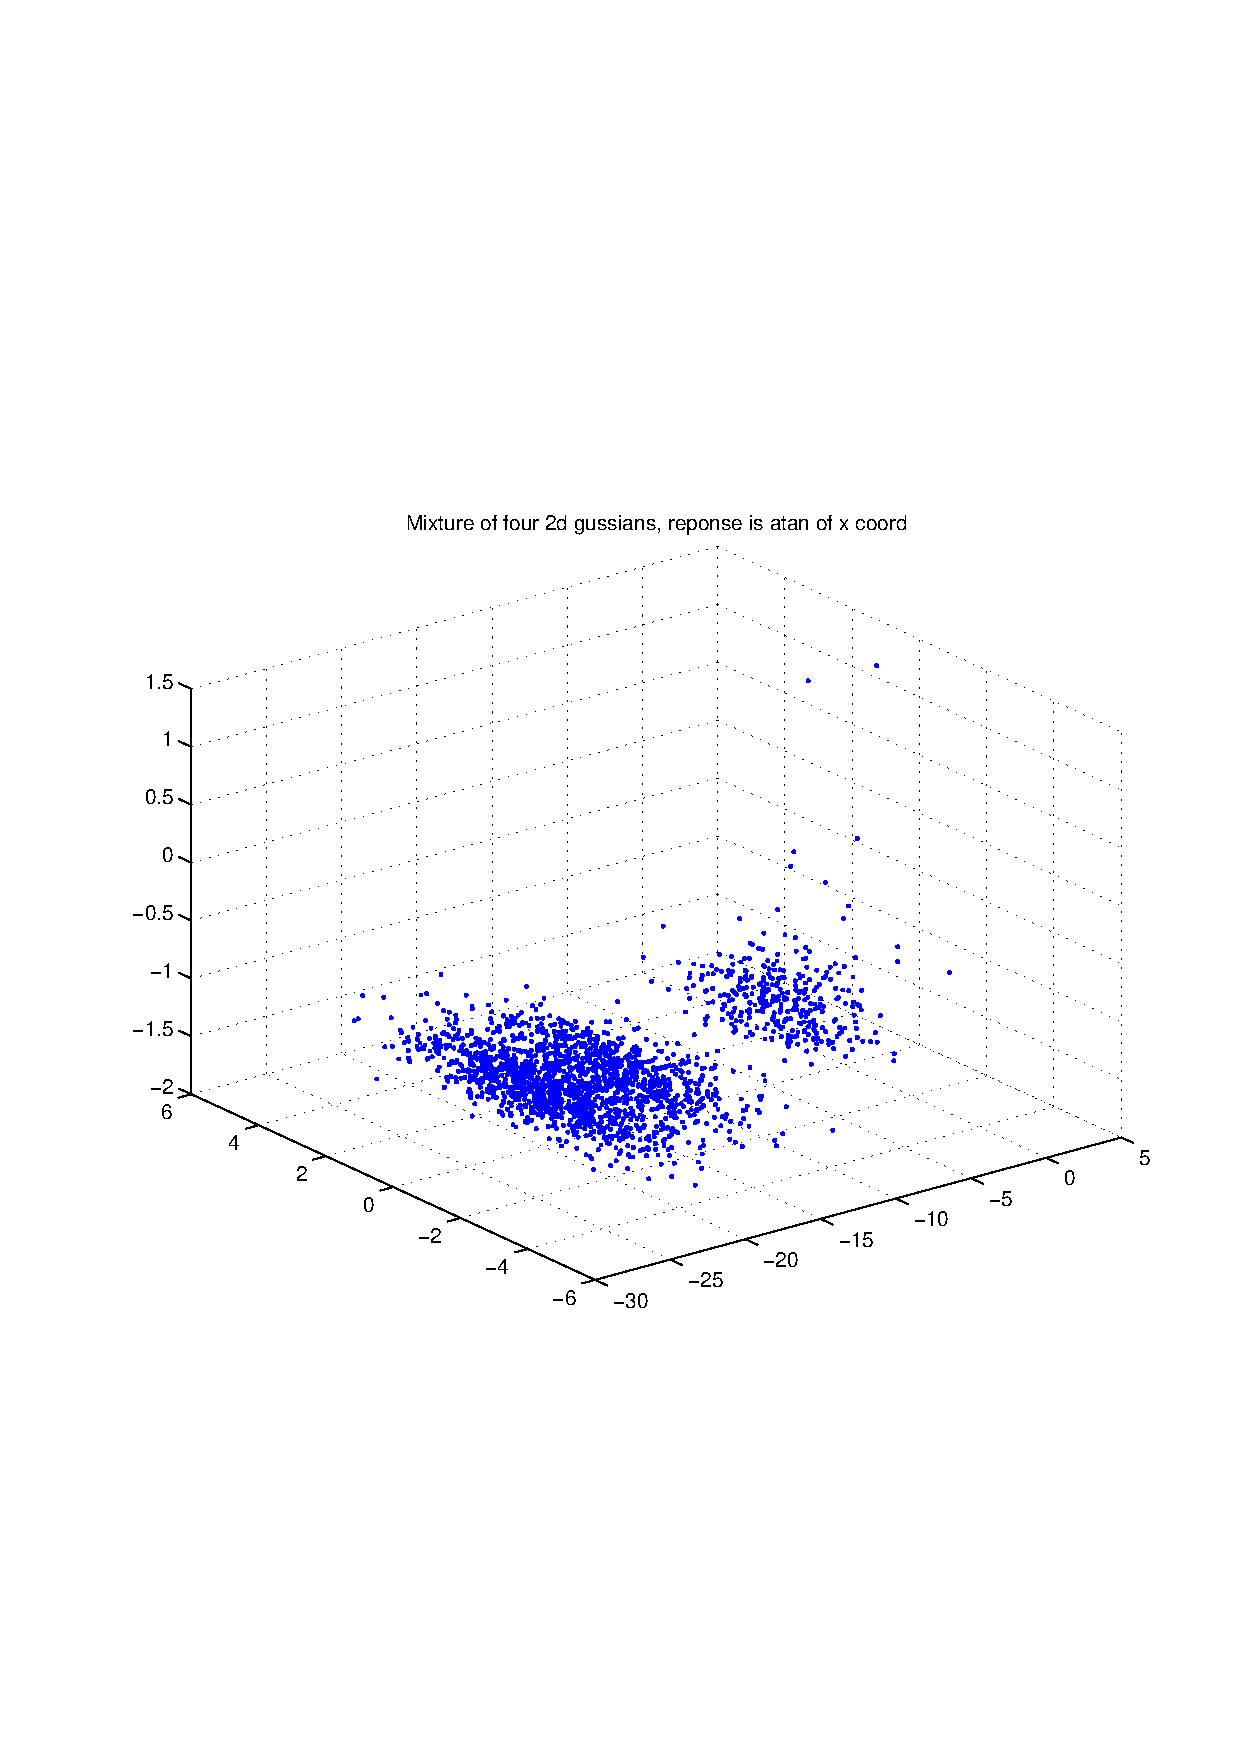
\includegraphics[width=10.0cm,height=10.0cm]{AtanDataSet.pdf}

\subsubsection{3 x 1 Linear Regression}
Sample size = 64

Number of features = 3

$\sigma = \left(
\begin{array}{
ccc}
+3.952 & -0.499 & -0.010 \\
-0.499 & +1.895 & +0.465 \\
-0.010 & +0.465 & +4.477 \\
\end{array}
\right)$ \newline 

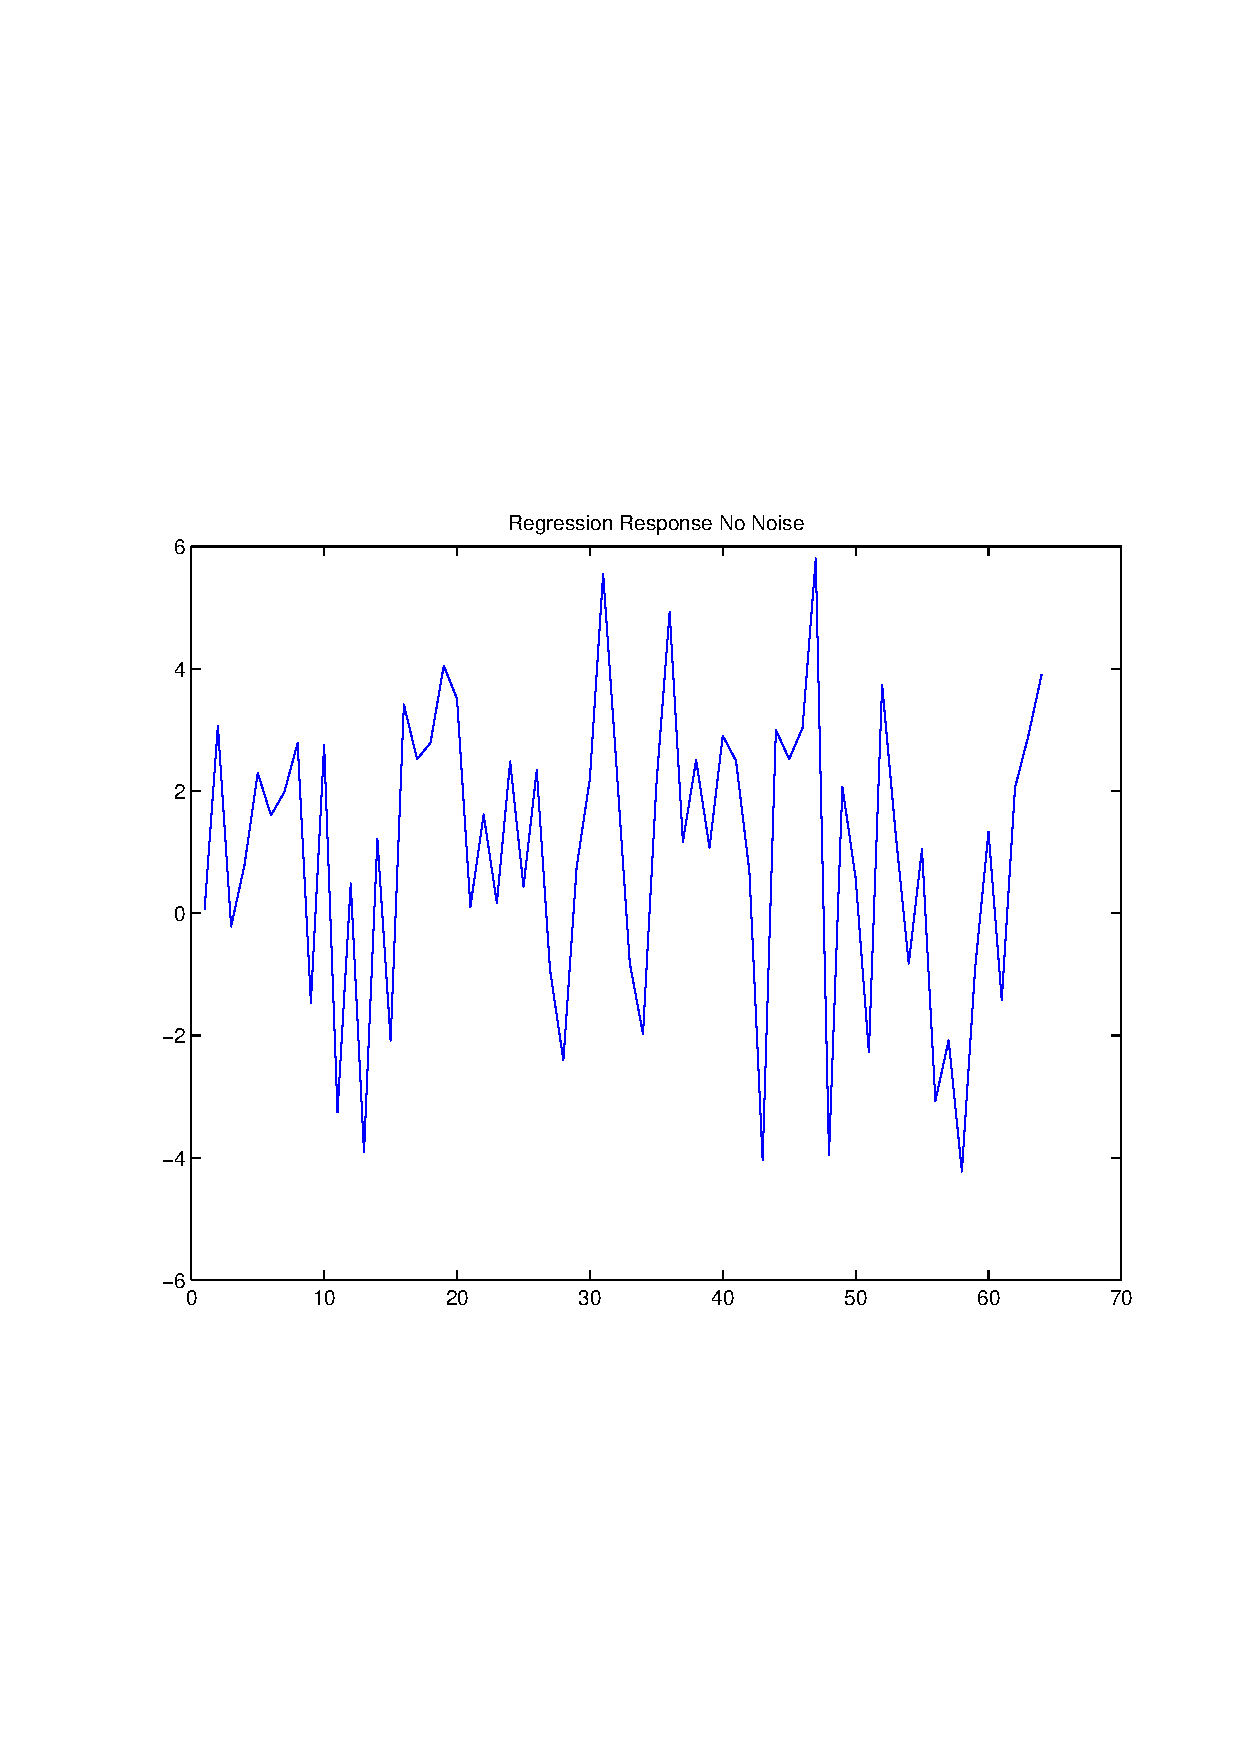
\includegraphics[width=10.0cm,height=10.0cm]{regression_response_no_noise.pdf}

\includegraphics[width=10.0cm,height=10.0cm]{regression_response_with_noise.pdf}

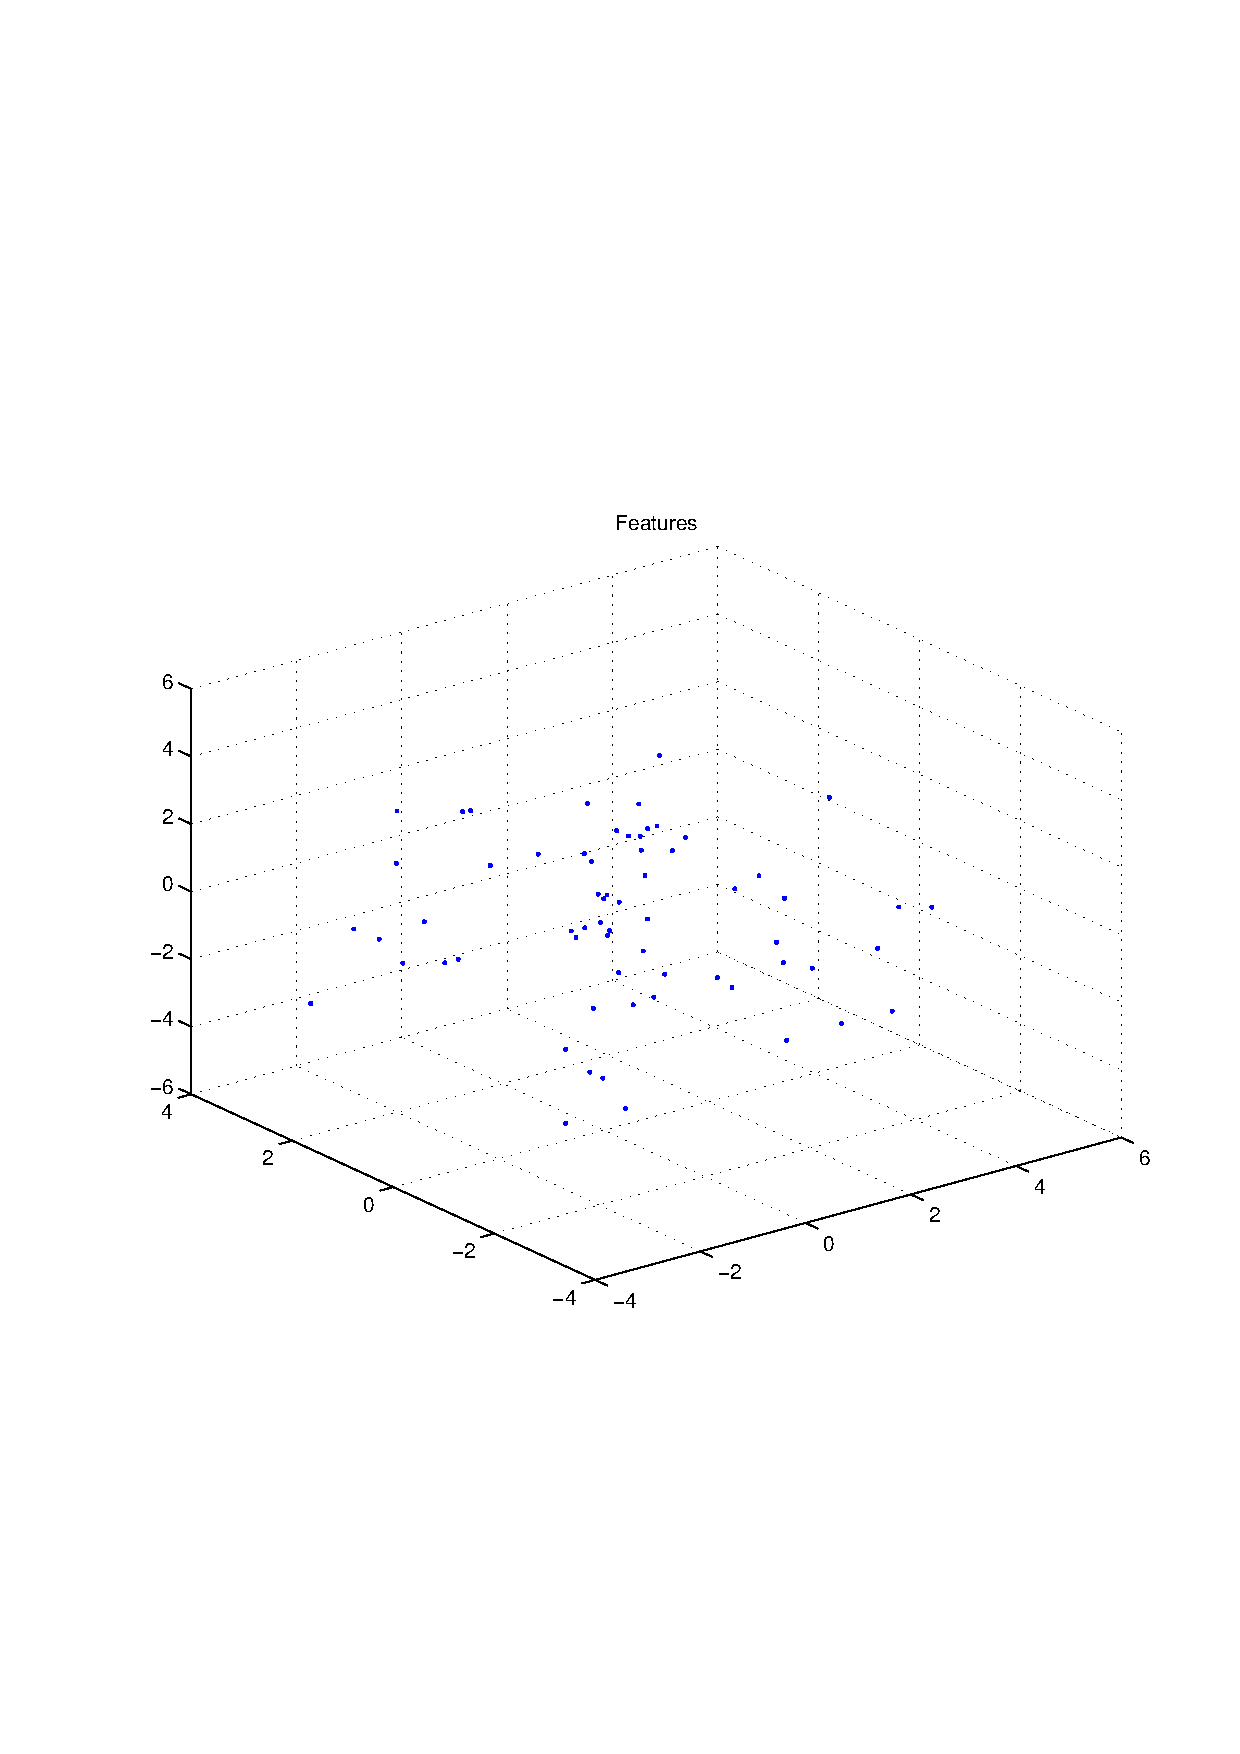
\includegraphics[width=10.0cm,height=10.0cm]{regression_features.pdf}

Beta
+0.817, +0.999, +0.510

Response
+1.037
+0.591
+4.804
+2.443
-0.921
+5.334
+3.388
+0.919
+0.169
+3.219
-0.311
+2.381
-0.812
+2.797
+0.229
+3.308
+0.633
+3.220
-2.895
+3.271
+3.014
+3.512
-0.928
-0.456
-1.254
+3.621
-0.567
+1.101
-2.307
+2.943
-1.823
-0.863
-2.233
+1.995
+2.145
+3.506
+1.599
-2.547
+1.755
+2.307
+0.964
+0.372
-2.221
+1.107
+2.781
+2.911
-1.430
-2.838
-1.712
-1.278
+2.957
-1.786
-0.177
-2.277
-1.124
+5.077
+1.194
+2.885
-2.330
+0.849
+0.787
+1.195
-0.964
-1.946
Estimate for Beta
+0.799
+1.018
+0.504
Error:
-0.019, +0.019, -0.006


QueryPerformanceCounter  =  +4.759
\subsubsection{Fast Gauss Transform}
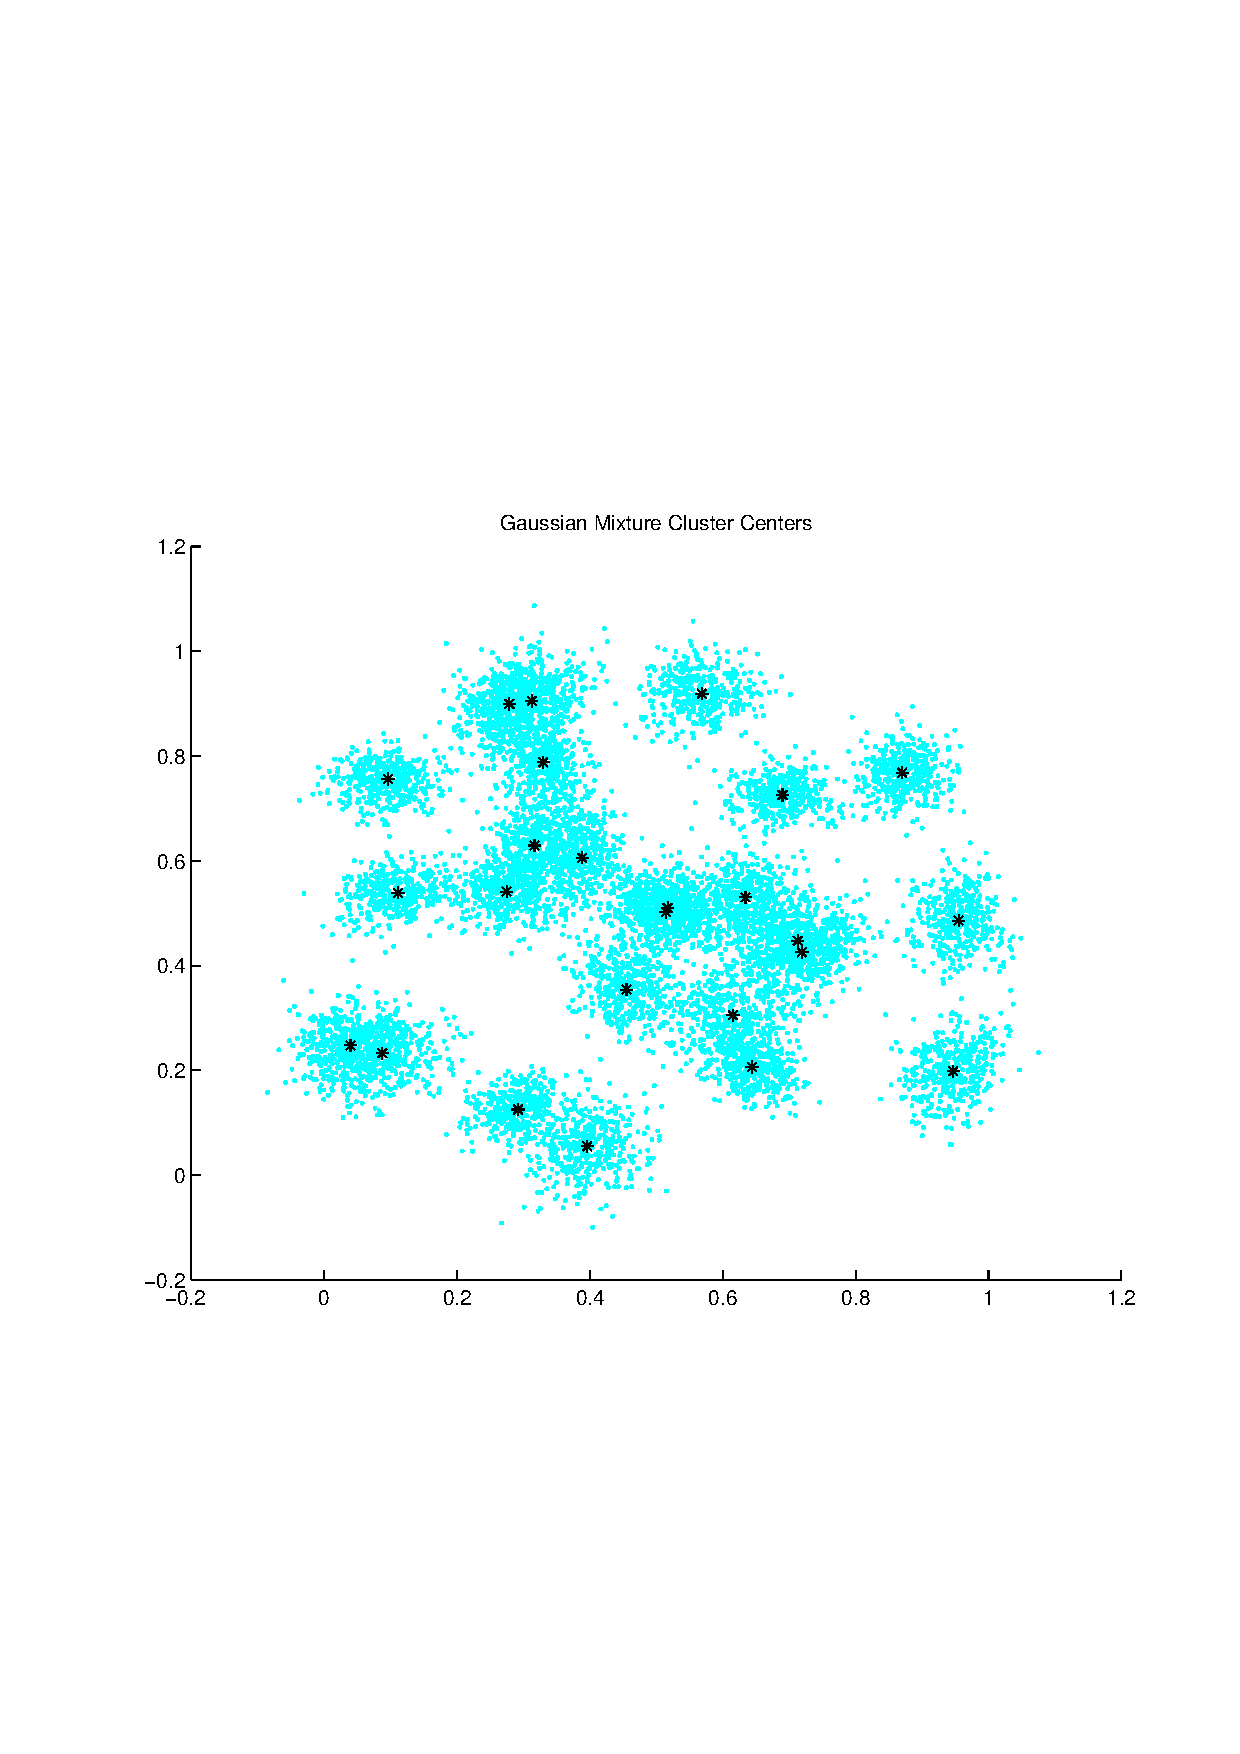
\includegraphics[width=10.0cm,height=10.0cm]{GaussianMixture_ClusterCenters25_Centers.pdf}

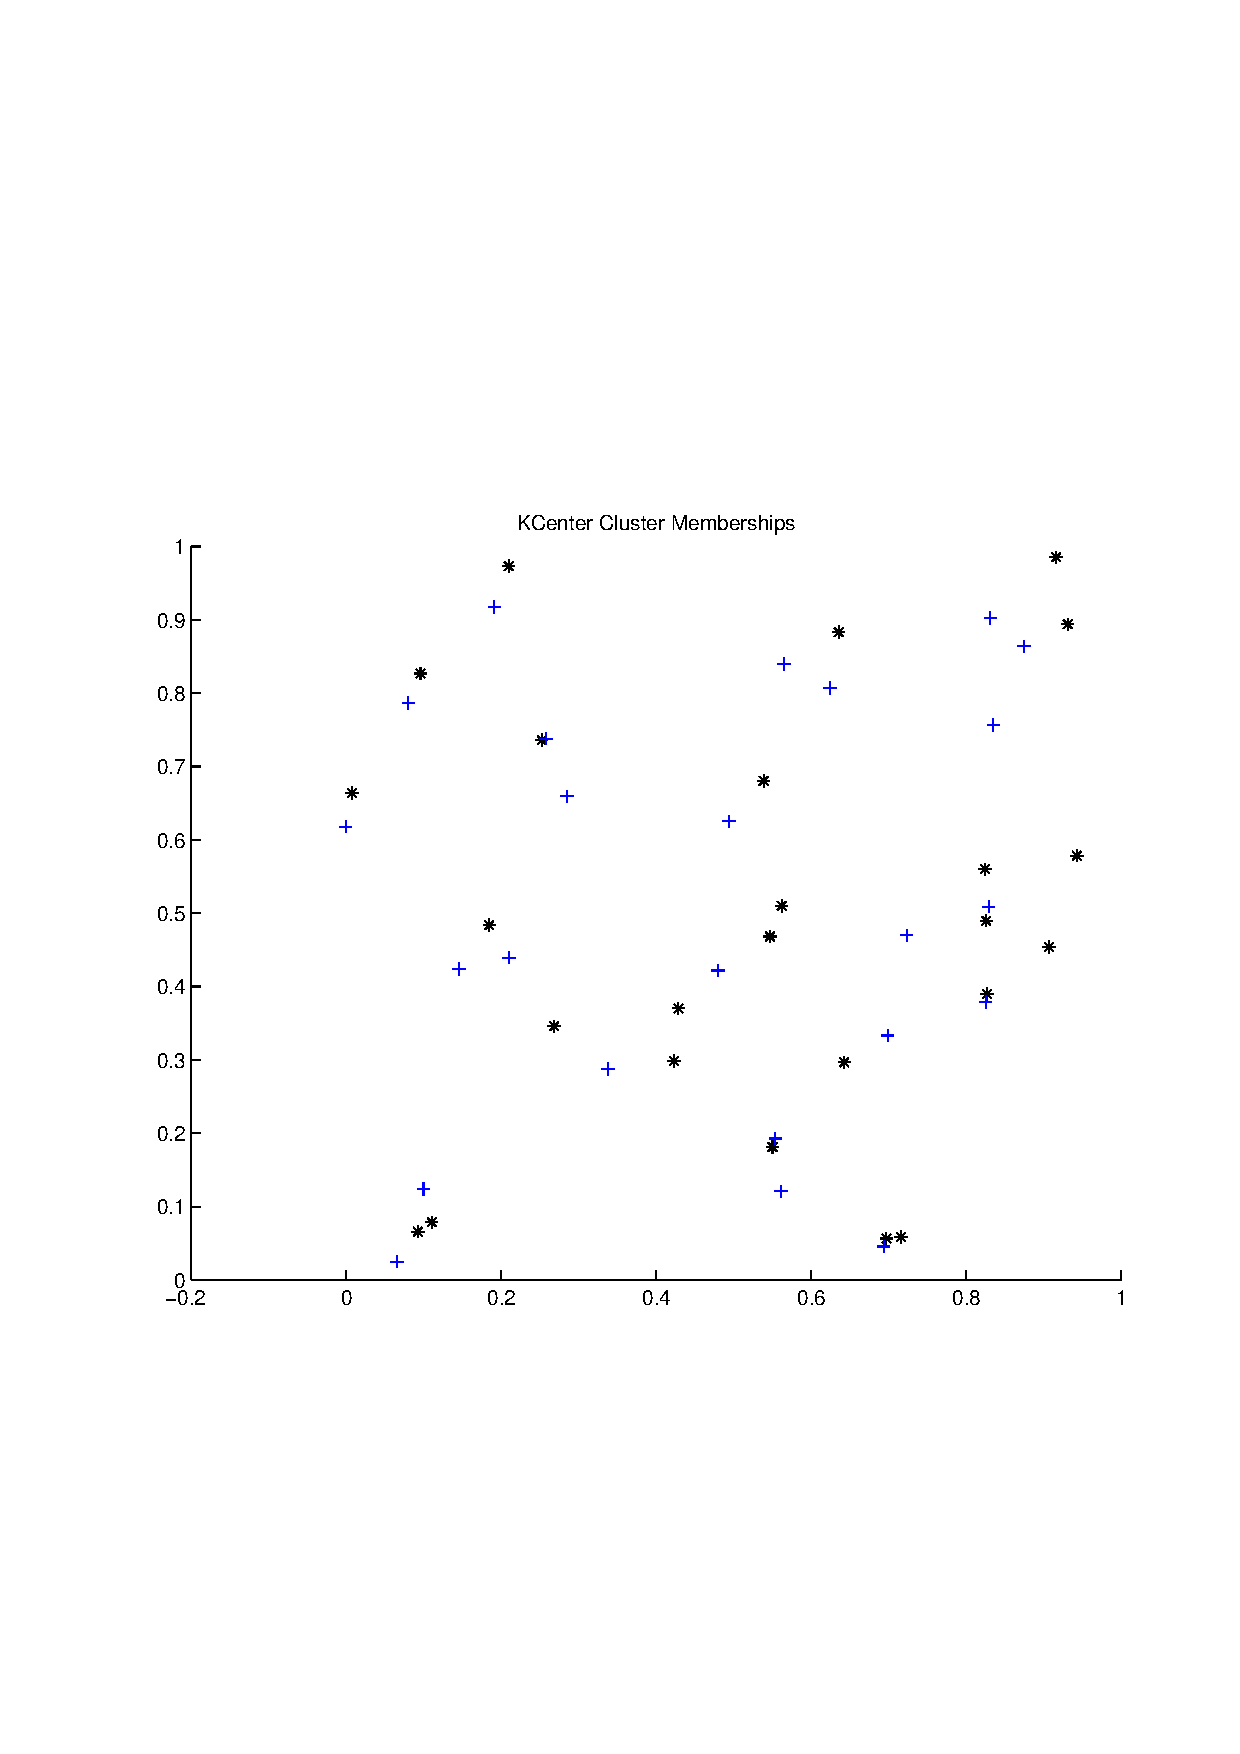
\includegraphics[width=10.0cm,height=10.0cm]{KCenterClusterMemberships_25_Centers.pdf}

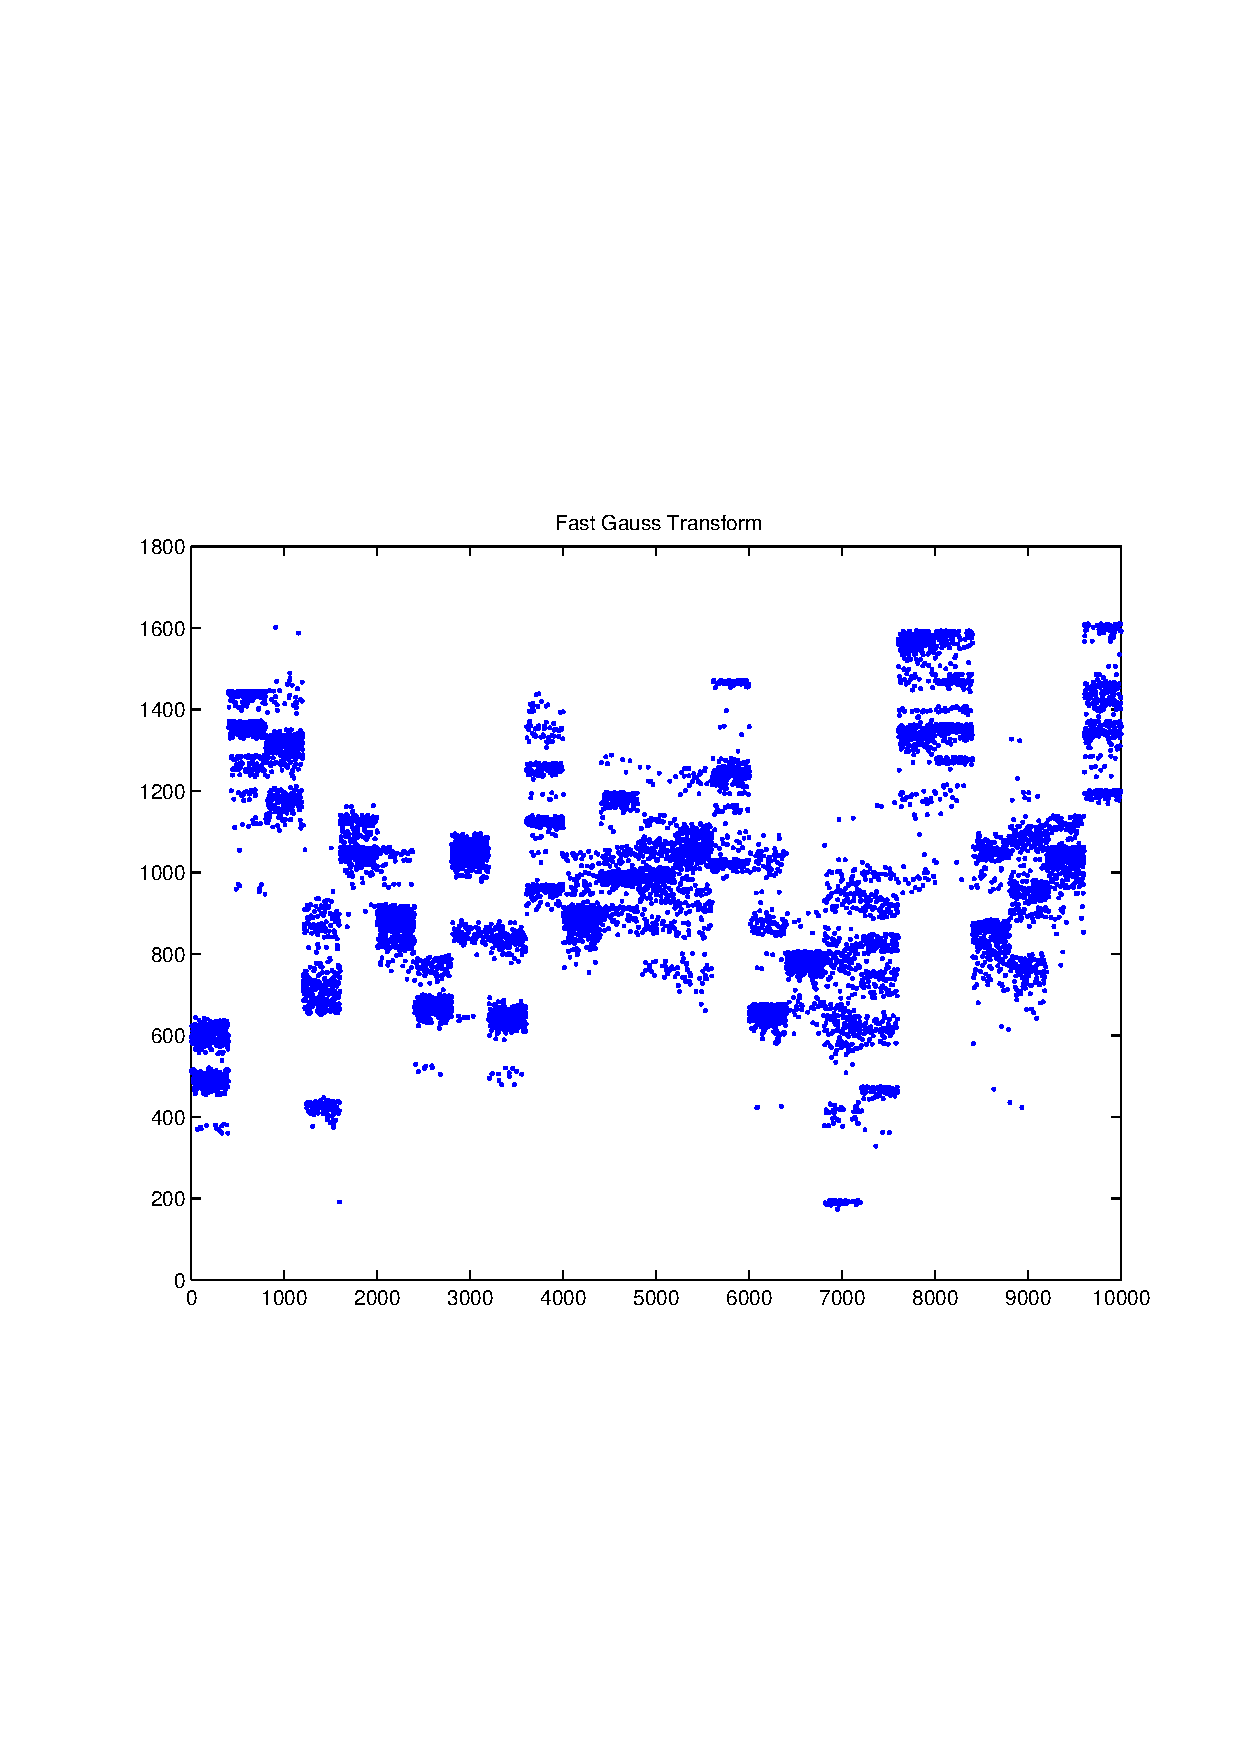
\includegraphics[width=10.0cm,height=10.0cm]{FGT25_Centers.pdf}

QueryPerformanceCounter  =  +6.845
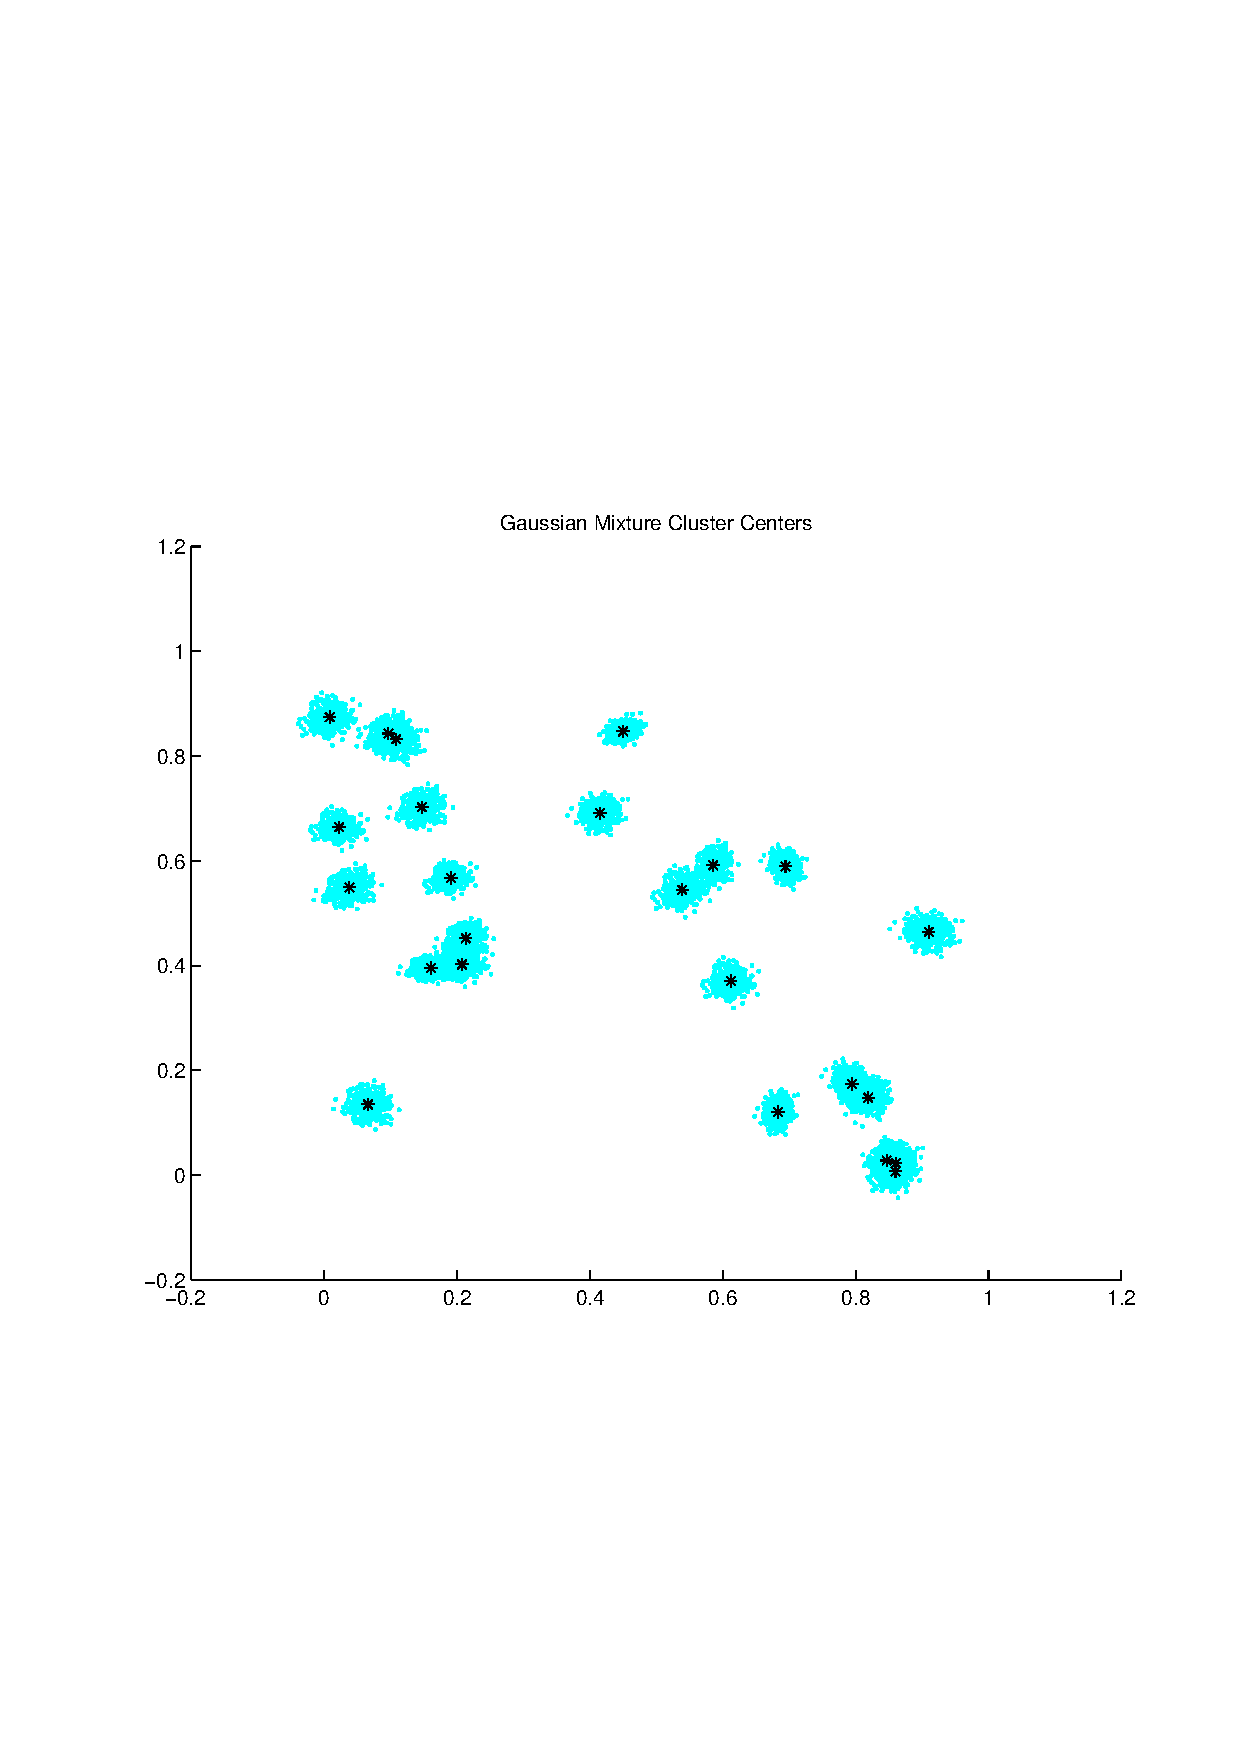
\includegraphics[width=10.0cm,height=10.0cm]{GaussianMixture_ClusterCenters24_Centers.pdf}

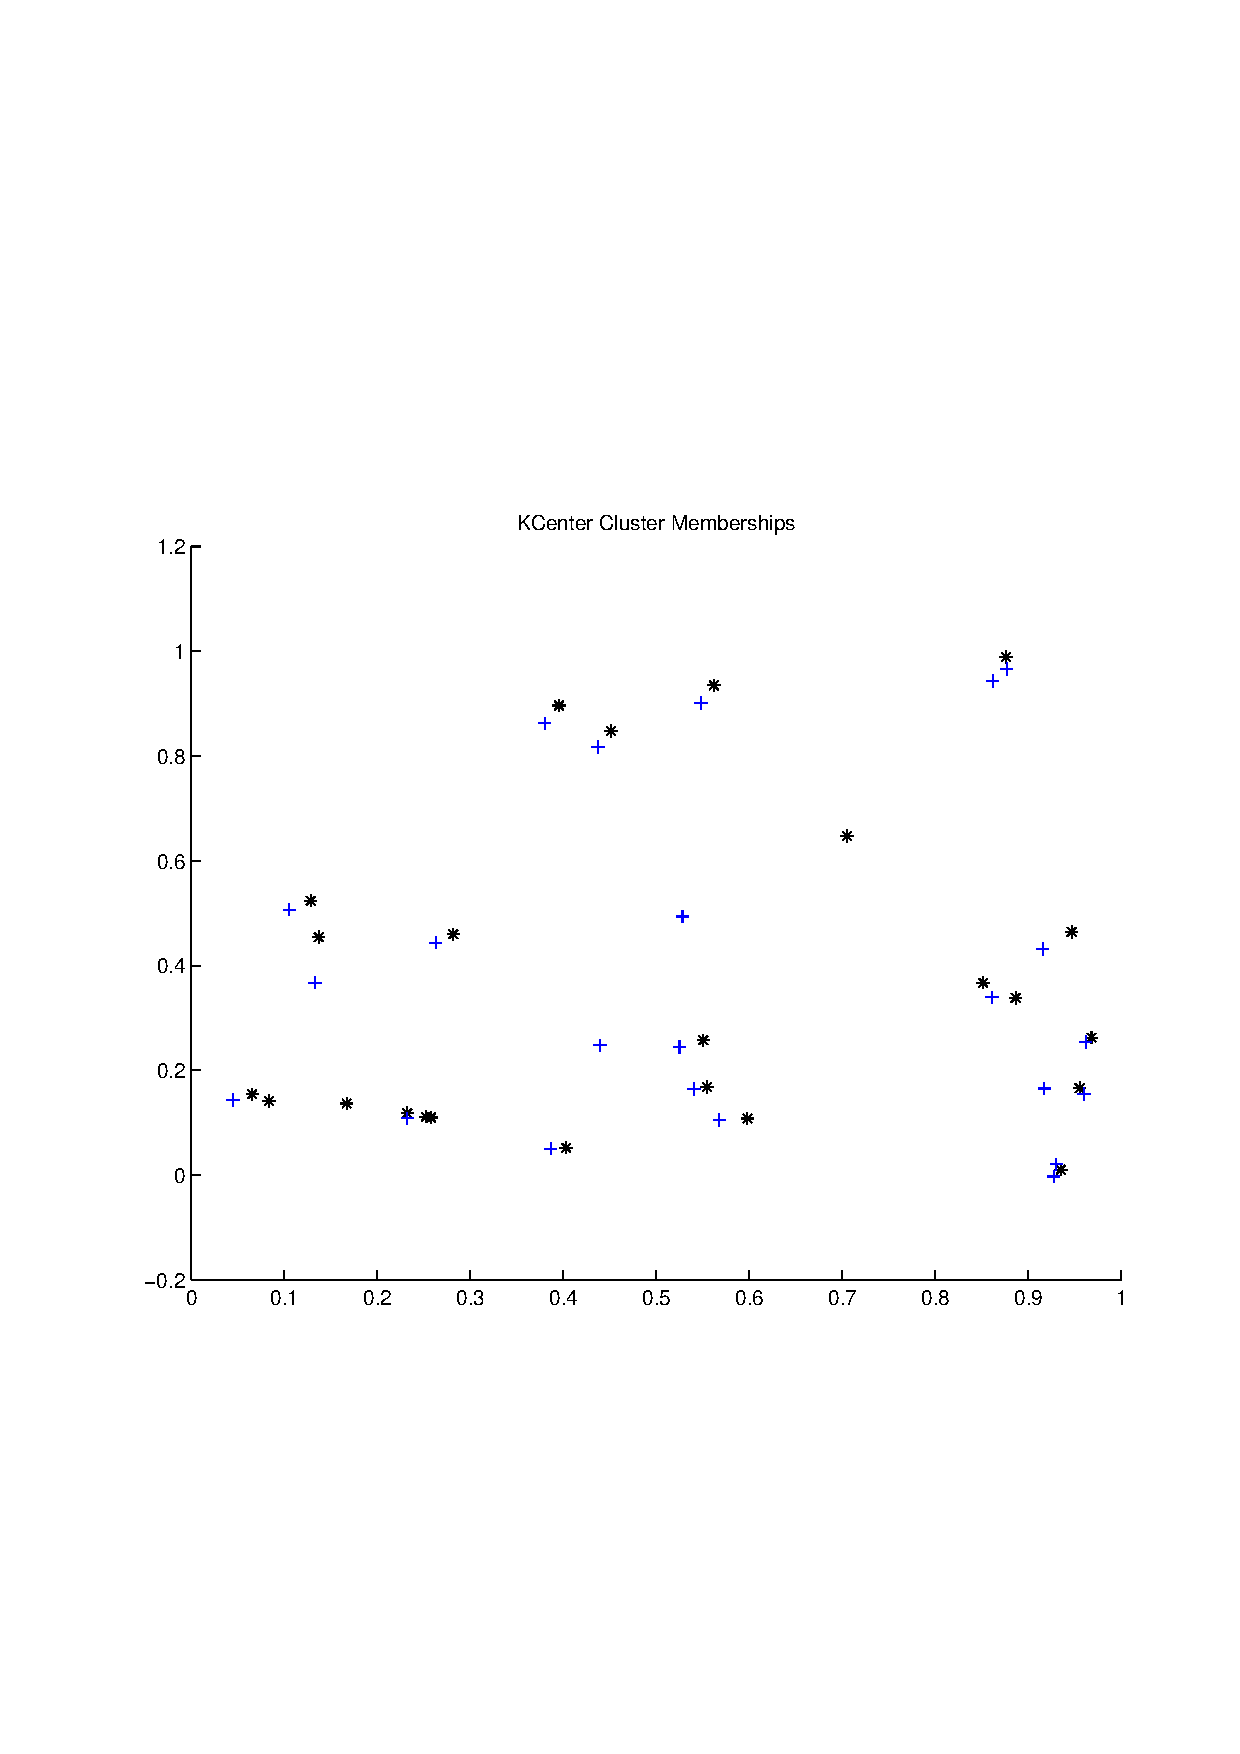
\includegraphics[width=10.0cm,height=10.0cm]{KCenterClusterMemberships_24_Centers.pdf}

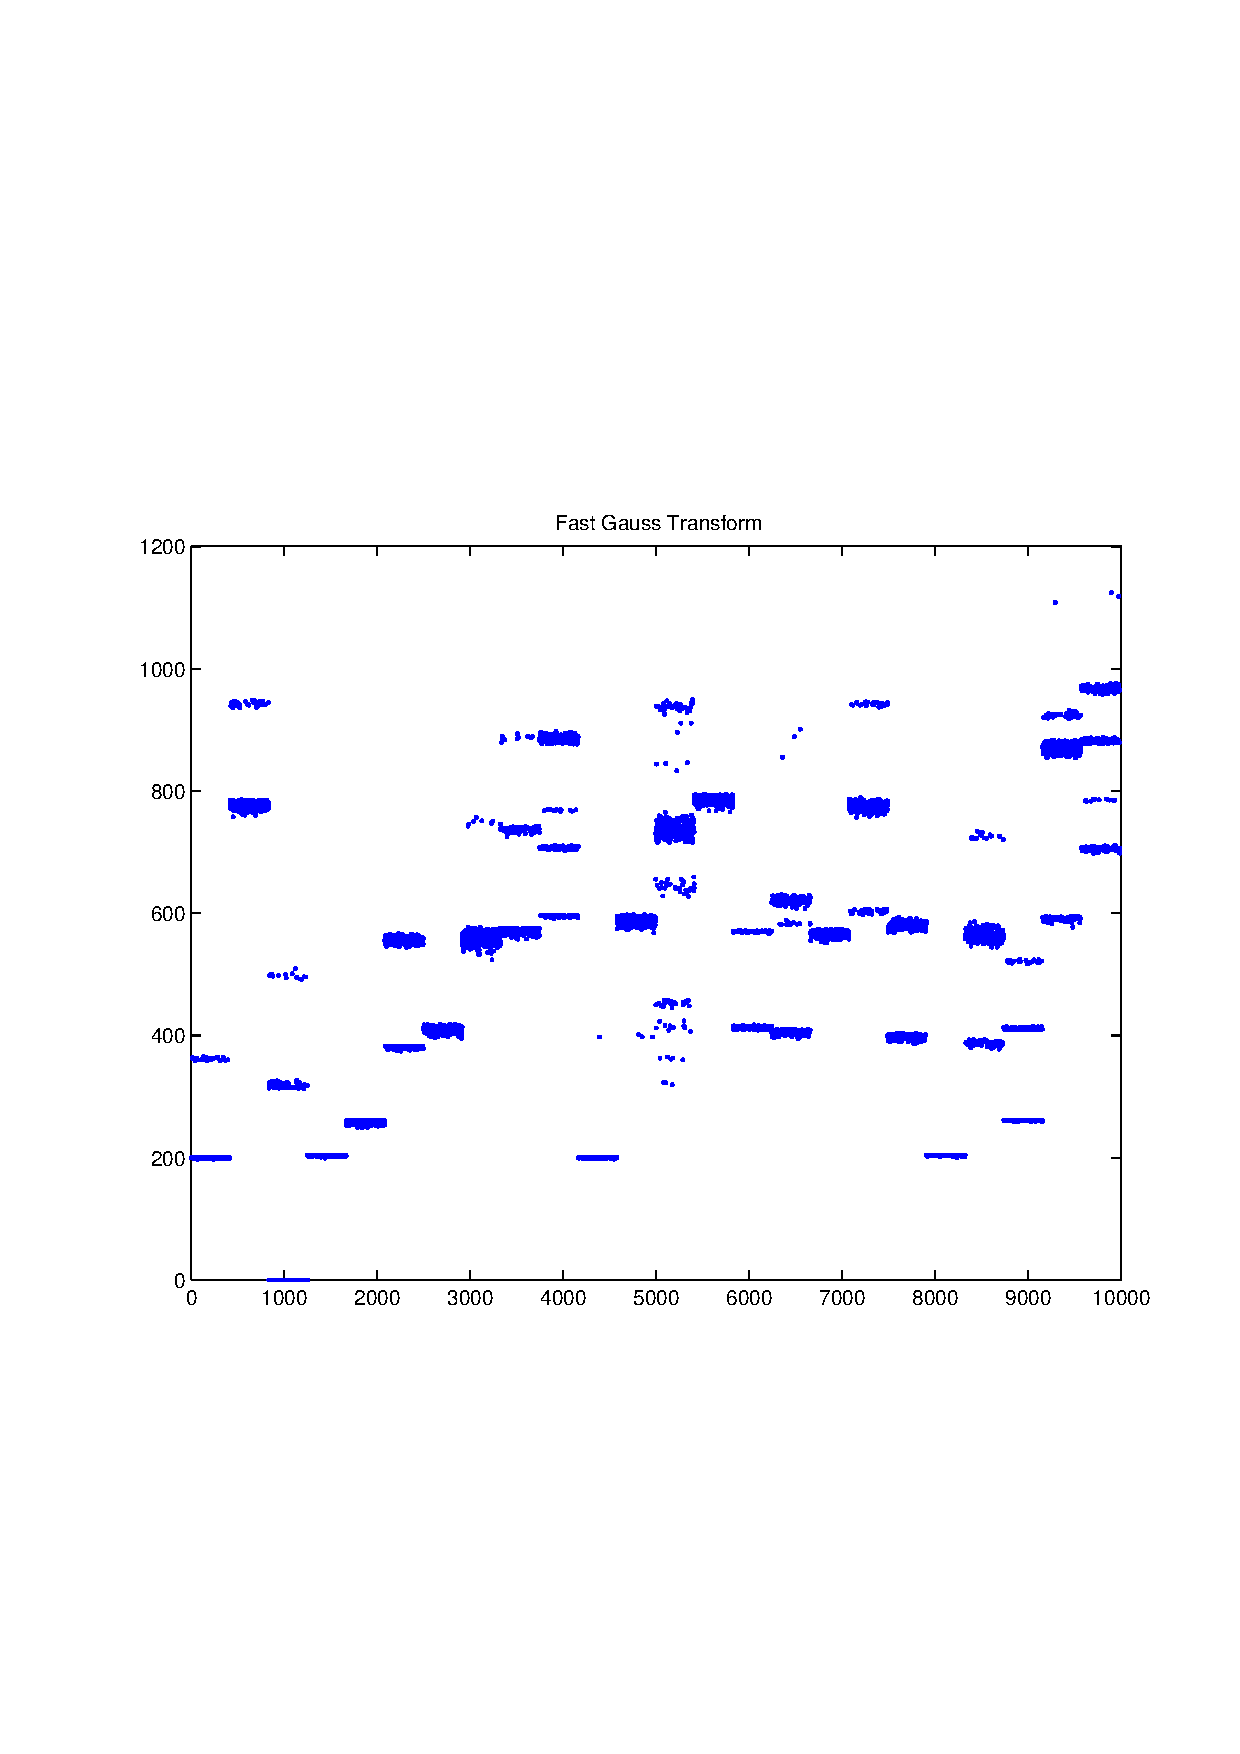
\includegraphics[width=10.0cm,height=10.0cm]{FGT24_Centers.pdf}

QueryPerformanceCounter  =  +7.776
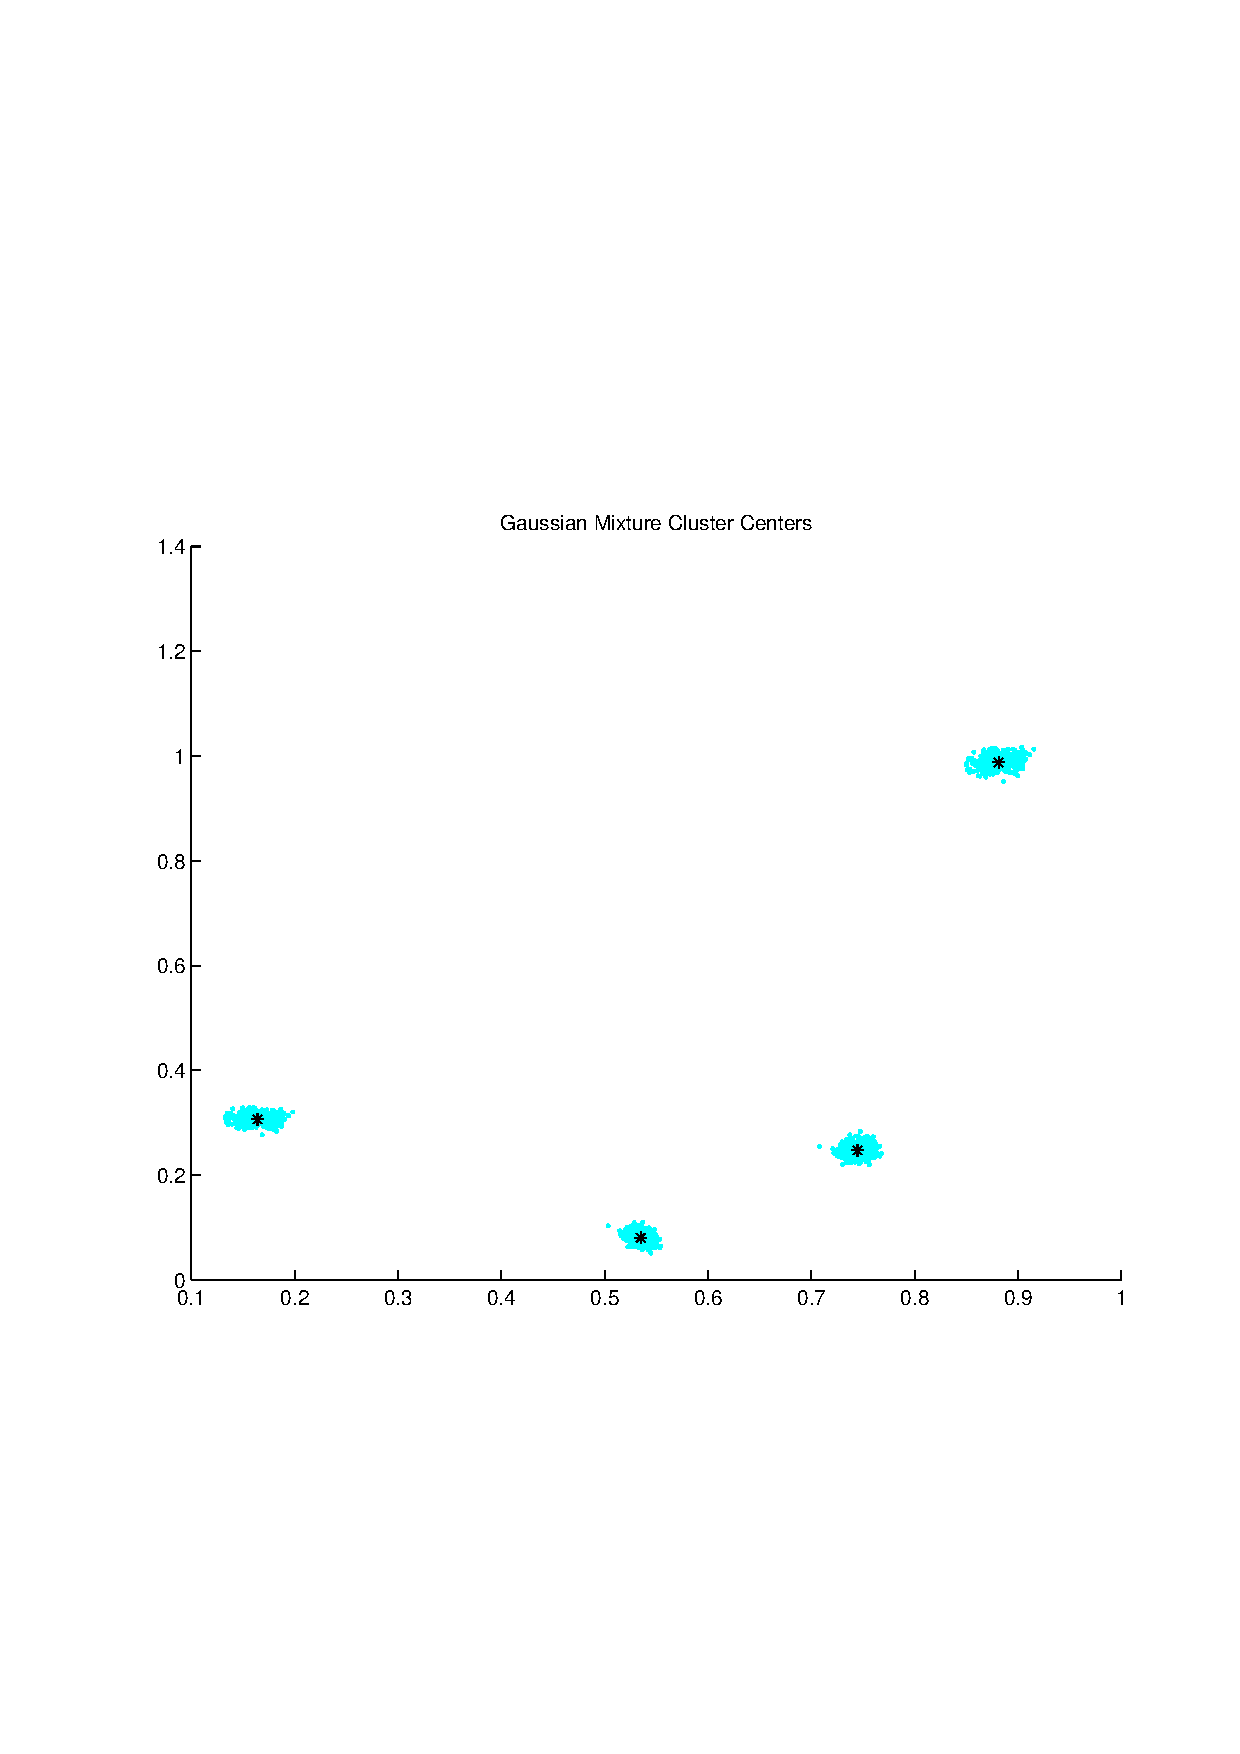
\includegraphics[width=10.0cm,height=10.0cm]{GaussianMixture_ClusterCenters4_Centers.pdf}

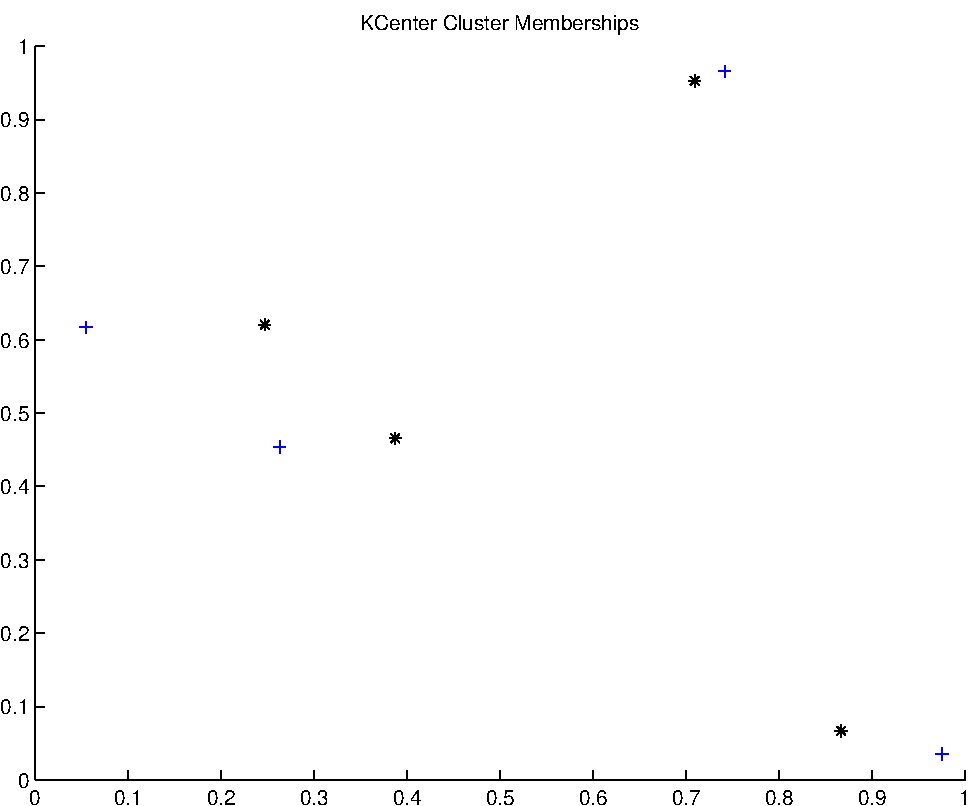
\includegraphics[width=10.0cm,height=10.0cm]{KCenterClusterMemberships_4_Centers.pdf}

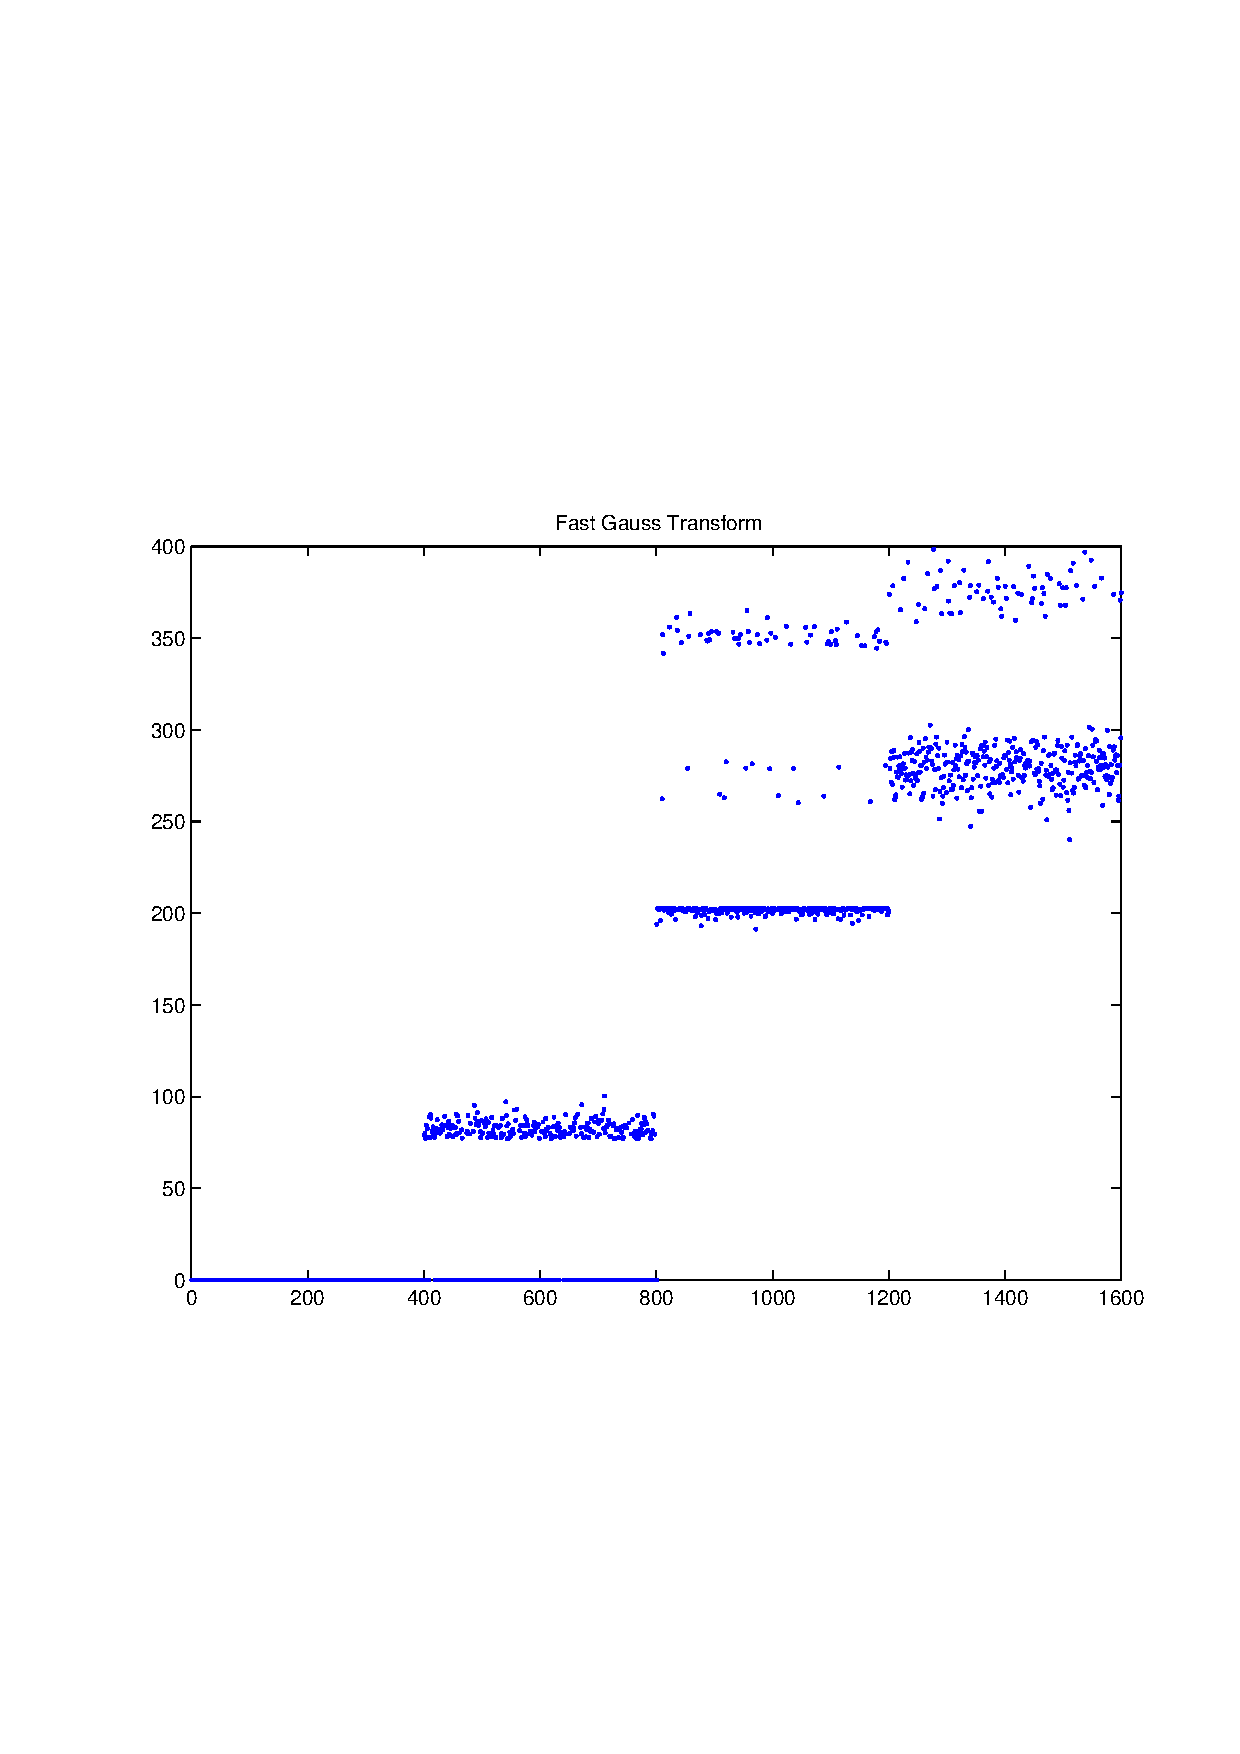
\includegraphics[width=10.0cm,height=10.0cm]{FGT4_Centers.pdf}

QueryPerformanceCounter  =  +3.916
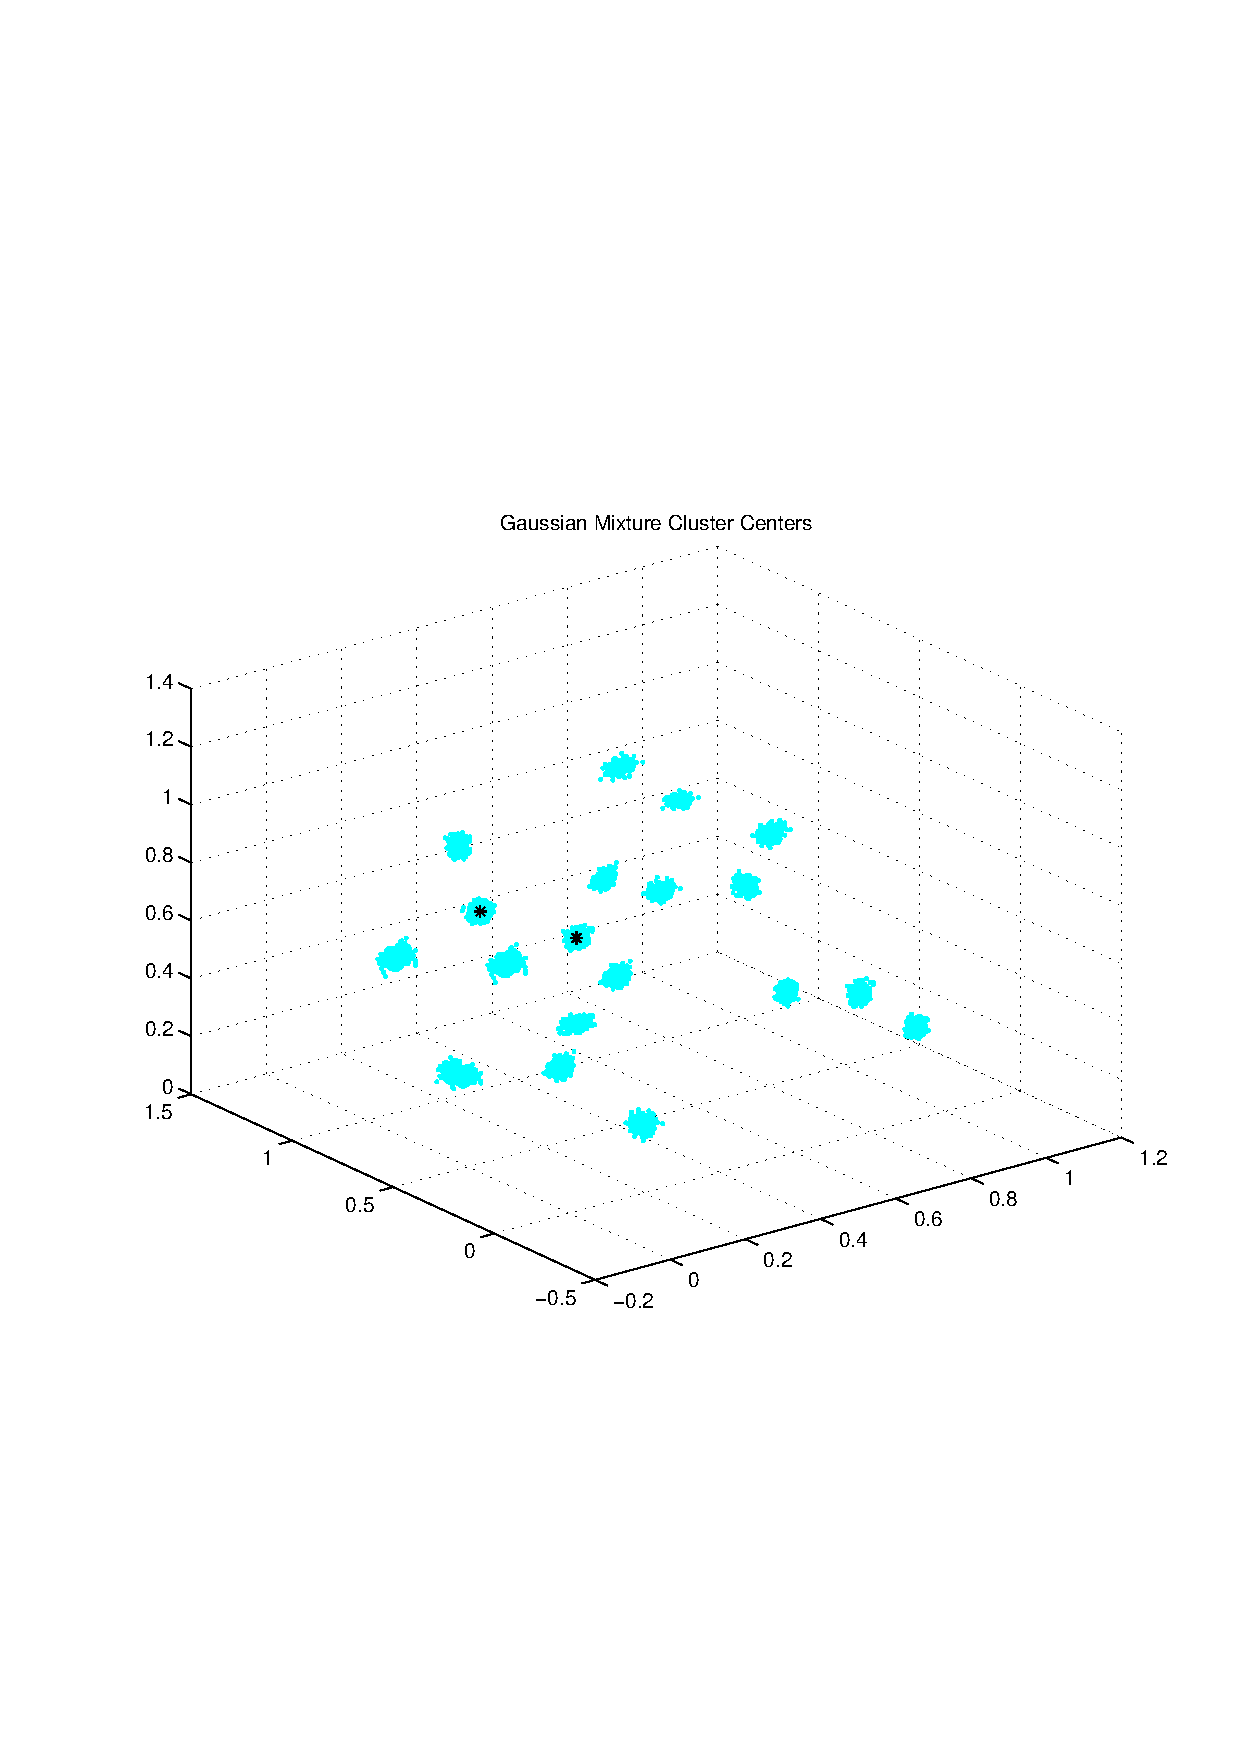
\includegraphics[width=10.0cm,height=10.0cm]{GaussianMixture_ClusterCenters20_Centers.pdf}

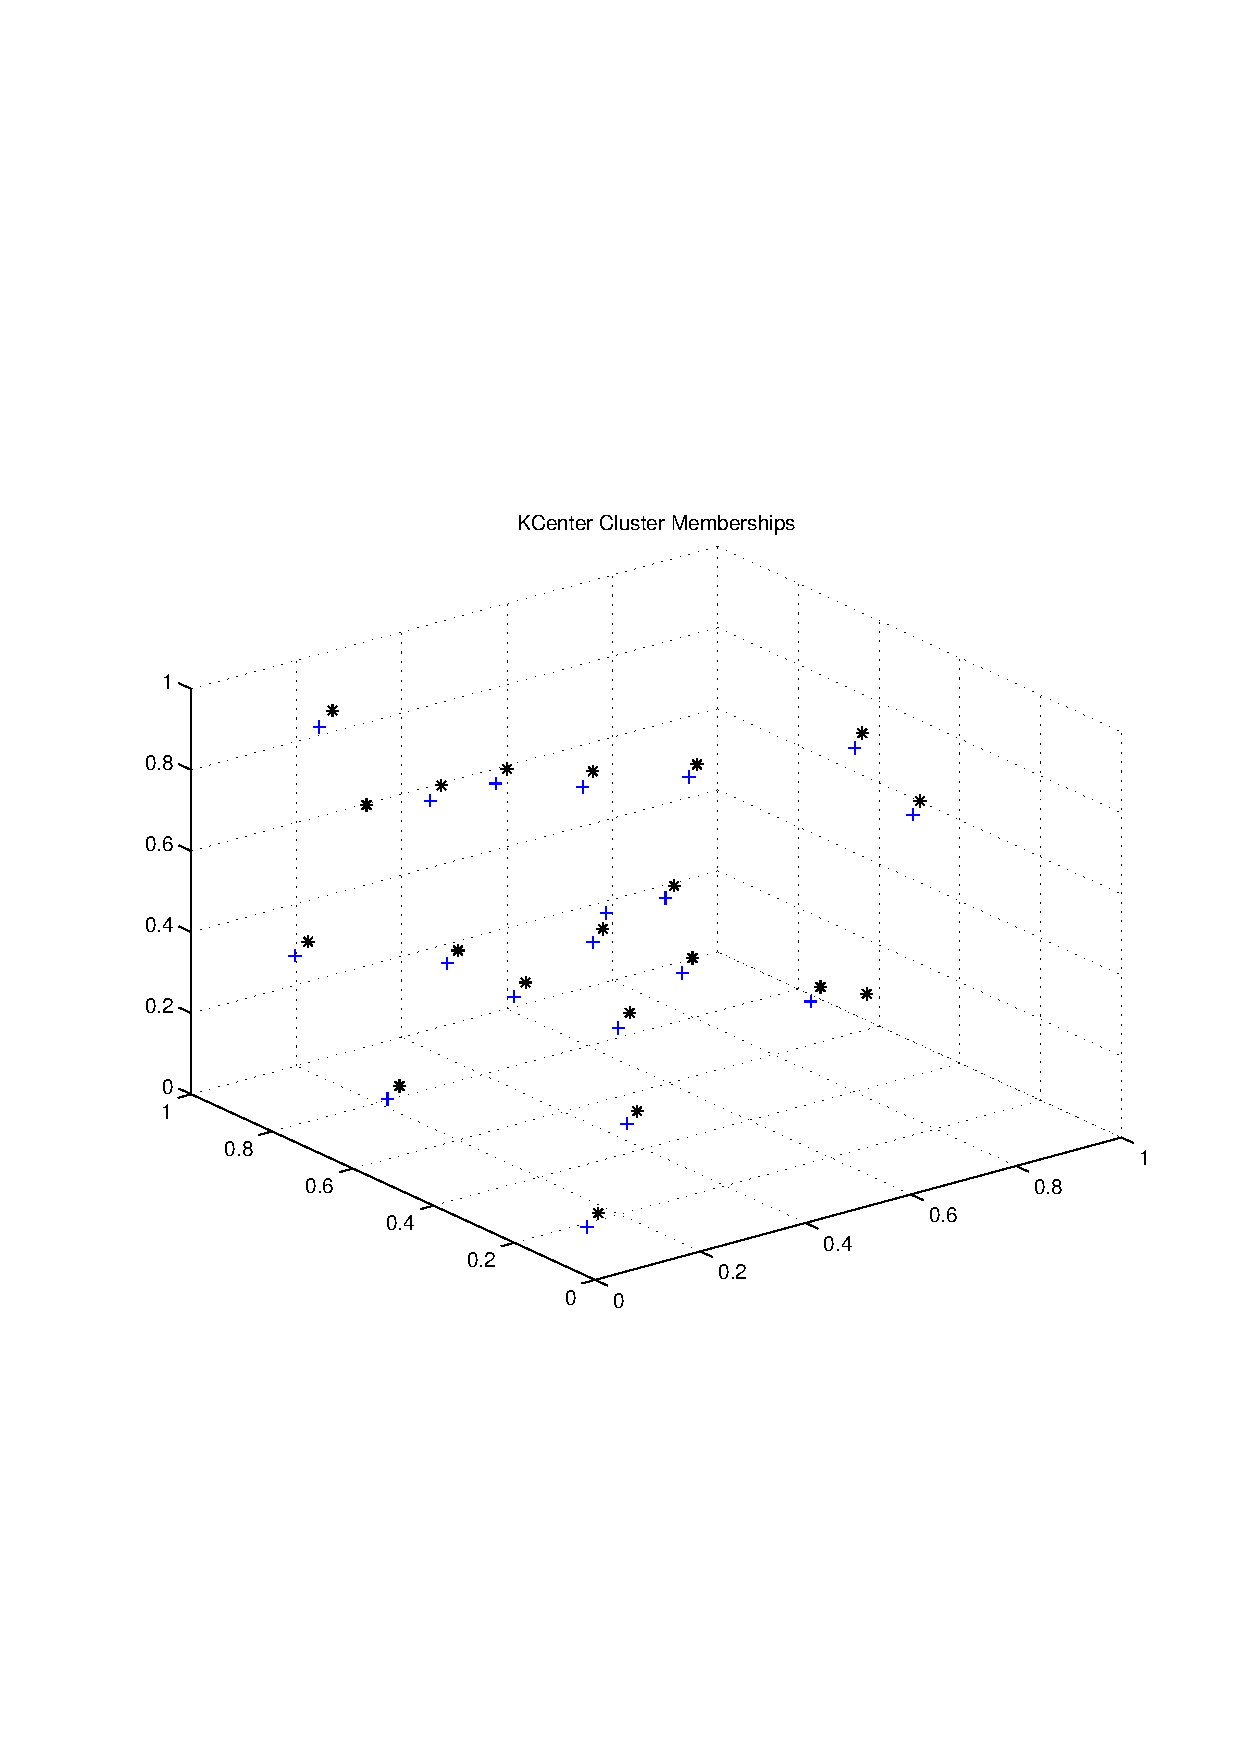
\includegraphics[width=10.0cm,height=10.0cm]{KCenterClusterMemberships_20_Centers.pdf}

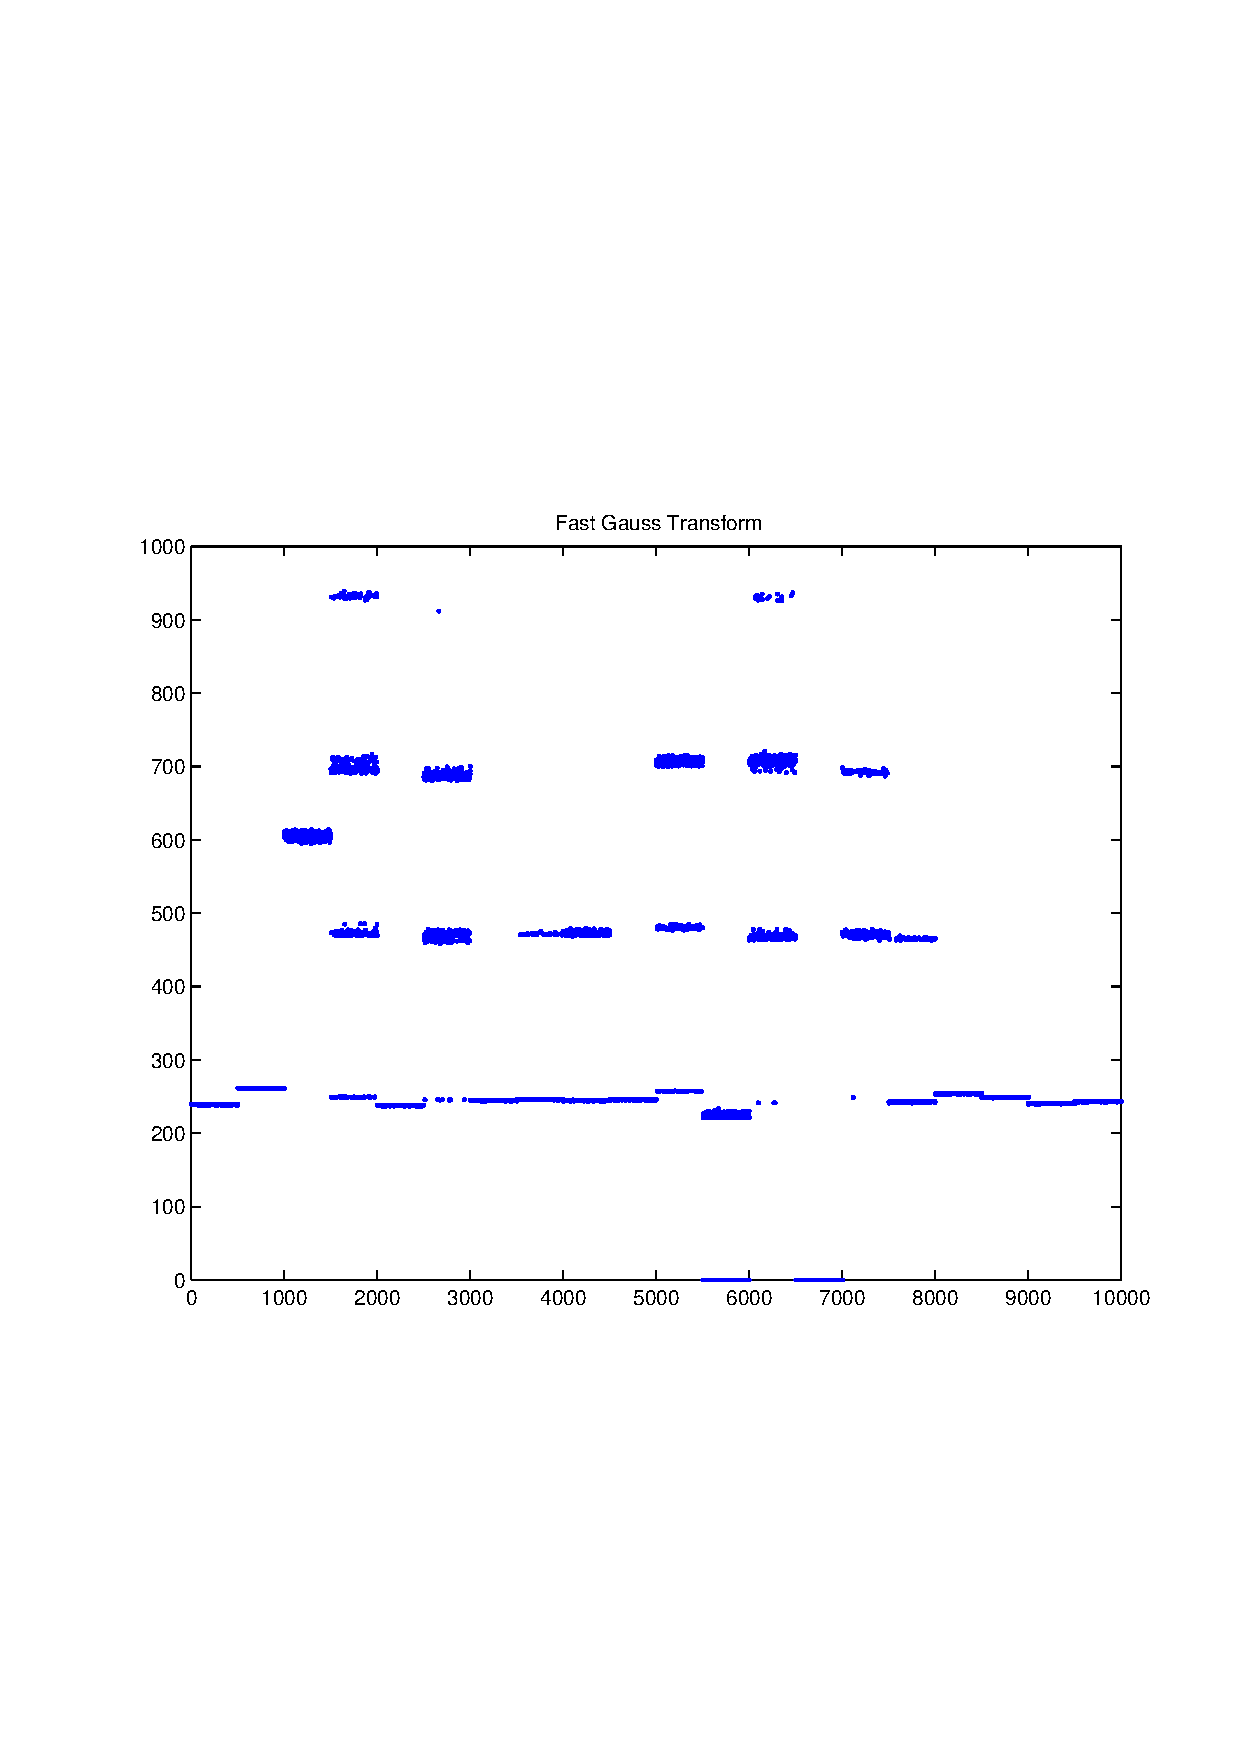
\includegraphics[width=10.0cm,height=10.0cm]{FGT20_Centers.pdf}

QueryPerformanceCounter  =  +6.317
\subsubsection{Matrix Norms}
\subsubsection{Haar Distributed Random Orthogonal Matrix $A \in O(n)$}
 Testing Operator Norm
Number of Dimensions: +12

$A = \left(
\begin{array}{
cccccccccccc}
+0.285 & +0.063 & +0.372 & -0.025 & +0.081 & +0.208 & -0.223 & -0.516 & -0.262 & -0.352 & +0.019 & +0.466 \\
-0.362 & -0.113 & -0.256 & -0.053 & +0.262 & +0.377 & -0.021 & +0.012 & -0.169 & +0.510 & +0.167 & +0.510 \\
+0.060 & -0.057 & -0.054 & -0.115 & +0.445 & +0.042 & -0.349 & -0.126 & -0.512 & +0.118 & +0.084 & -0.597 \\
-0.037 & -0.401 & -0.427 & +0.466 & -0.056 & +0.130 & +0.330 & -0.228 & -0.282 & -0.268 & -0.321 & -0.050 \\
+0.257 & +0.137 & -0.418 & -0.200 & -0.209 & -0.387 & -0.007 & +0.304 & -0.500 & -0.158 & +0.248 & +0.279 \\
+0.237 & -0.455 & +0.119 & -0.037 & -0.120 & +0.487 & -0.283 & +0.593 & +0.009 & -0.196 & -0.008 & +0.001 \\
-0.299 & +0.181 & -0.174 & +0.498 & -0.349 & +0.024 & -0.609 & -0.084 & +0.070 & -0.090 & +0.288 & -0.051 \\
+0.038 & +0.381 & -0.009 & -0.219 & -0.575 & +0.509 & +0.188 & -0.111 & -0.253 & +0.198 & -0.116 & -0.229 \\
-0.457 & -0.047 & -0.047 & -0.401 & -0.102 & -0.164 & -0.356 & +0.016 & -0.080 & -0.157 & -0.648 & +0.102 \\
-0.051 & +0.082 & +0.519 & +0.469 & -0.058 & -0.213 & +0.041 & +0.300 & -0.428 & +0.319 & -0.259 & +0.098 \\
+0.353 & -0.490 & -0.032 & -0.080 & -0.368 & -0.254 & -0.225 & -0.321 & +0.088 & +0.513 & -0.055 & +0.026 \\
+0.484 & +0.408 & -0.346 & +0.204 & +0.254 & +0.113 & -0.233 & +0.096 & +0.210 & +0.172 & -0.462 & +0.104 \\
\end{array}
\right)$ \newline 

$Det(A) :   A \in O(n)$ = (-1.000,+0.000)

$L = \left(
\begin{array}{
cccccccccccc}
+1.000 & +0.000 & +0.000 & +0.000 & +0.000 & +0.000 & +0.000 & +0.000 & +0.000 & +0.000 & +0.000 & +0.000 \\
+0.730 & +1.000 & +0.000 & +0.000 & +0.000 & +0.000 & +0.000 & +0.000 & +0.000 & +0.000 & +0.000 & +0.000 \\
-0.076 & +0.470 & +1.000 & +0.000 & +0.000 & +0.000 & +0.000 & +0.000 & +0.000 & +0.000 & +0.000 & +0.000 \\
-0.106 & -0.159 & -0.930 & +1.000 & +0.000 & +0.000 & +0.000 & +0.000 & +0.000 & +0.000 & +0.000 & +0.000 \\
+0.079 & -0.442 & -0.208 & -0.214 & +1.000 & +0.000 & +0.000 & +0.000 & +0.000 & +0.000 & +0.000 & +0.000 \\
+0.490 & +0.831 & -0.189 & +0.165 & -0.314 & +1.000 & +0.000 & +0.000 & +0.000 & +0.000 & +0.000 & +0.000 \\
-0.618 & -0.550 & +0.479 & +0.216 & +0.804 & -0.641 & +1.000 & +0.000 & +0.000 & +0.000 & +0.000 & +0.000 \\
+0.530 & +0.101 & +0.462 & -0.556 & +0.441 & -0.808 & +0.005 & +1.000 & +0.000 & +0.000 & +0.000 & +0.000 \\
+0.125 & +0.137 & +0.073 & -0.152 & -0.629 & +0.356 & +0.064 & -0.439 & +1.000 & +0.000 & +0.000 & +0.000 \\
+0.588 & +0.225 & -0.945 & +0.463 & -0.291 & +0.681 & -0.155 & -0.995 & +0.792 & +1.000 & +0.000 & +0.000 \\
-0.945 & -0.429 & +0.501 & -0.601 & +0.204 & -0.472 & +0.505 & +0.245 & +0.255 & -0.197 & +1.000 & +0.000 \\
-0.748 & -0.244 & +0.828 & -0.444 & -0.222 & +0.263 & +0.212 & -0.200 & +0.394 & -0.875 & -0.201 & +1.000 \\
\end{array}
\right)$ \newline 

$U = \left(
\begin{array}{
cccccccccccc}
+0.484 & +0.408 & -0.346 & +0.204 & +0.254 & +0.113 & -0.233 & +0.096 & +0.210 & +0.172 & -0.462 & +0.104 \\
+0.000 & -0.788 & +0.220 & -0.229 & -0.553 & -0.336 & -0.055 & -0.391 & -0.065 & +0.387 & +0.282 & -0.049 \\
+0.000 & +0.000 & -0.556 & +0.590 & +0.223 & +0.297 & +0.338 & -0.037 & -0.236 & -0.437 & -0.488 & -0.019 \\
+0.000 & +0.000 & +0.000 & +1.002 & +0.089 & +0.022 & +0.322 & +0.213 & -0.635 & -0.008 & -0.717 & +0.083 \\
+0.000 & +0.000 & +0.000 & +0.000 & -0.774 & +0.418 & +0.321 & -0.254 & -0.483 & +0.263 & -0.209 & -0.245 \\
+0.000 & +0.000 & +0.000 & +0.000 & +0.000 & +0.895 & -0.012 & +0.749 & -0.132 & -0.601 & -0.056 & -0.103 \\
+0.000 & +0.000 & +0.000 & +0.000 & +0.000 & +0.000 & -1.280 & +0.417 & +0.718 & -0.156 & +0.679 & +0.109 \\
+0.000 & +0.000 & +0.000 & +0.000 & +0.000 & +0.000 & +0.000 & +1.144 & -0.746 & -0.692 & +0.336 & +0.308 \\
+0.000 & +0.000 & +0.000 & +0.000 & +0.000 & +0.000 & +0.000 & +0.000 & -1.239 & +0.159 & +0.022 & -0.578 \\
+0.000 & +0.000 & +0.000 & +0.000 & +0.000 & +0.000 & +0.000 & +0.000 & +0.000 & -1.303 & +0.496 & +1.140 \\
+0.000 & +0.000 & +0.000 & +0.000 & +0.000 & +0.000 & +0.000 & +0.000 & +0.000 & +0.000 & -1.466 & +0.481 \\
+0.000 & +0.000 & +0.000 & +0.000 & +0.000 & +0.000 & +0.000 & +0.000 & +0.000 & +0.000 & +0.000 & +1.961 \\
\end{array}
\right)$ \newline 

$L * U  = \left(
\begin{array}{
cccccccccccc}
+0.484 & +0.408 & -0.346 & +0.204 & +0.254 & +0.113 & -0.233 & +0.096 & +0.210 & +0.172 & -0.462 & +0.104 \\
+0.353 & -0.490 & -0.032 & -0.080 & -0.368 & -0.254 & -0.225 & -0.321 & +0.088 & +0.513 & -0.055 & +0.026 \\
-0.037 & -0.401 & -0.427 & +0.466 & -0.056 & +0.130 & +0.330 & -0.228 & -0.282 & -0.268 & -0.321 & -0.050 \\
-0.051 & +0.082 & +0.519 & +0.469 & -0.058 & -0.213 & +0.041 & +0.300 & -0.428 & +0.319 & -0.259 & +0.098 \\
+0.038 & +0.381 & -0.009 & -0.219 & -0.575 & +0.509 & +0.188 & -0.111 & -0.253 & +0.198 & -0.116 & -0.229 \\
+0.237 & -0.455 & +0.119 & -0.037 & -0.120 & +0.487 & -0.283 & +0.593 & +0.009 & -0.196 & -0.008 & +0.001 \\
-0.299 & +0.181 & -0.174 & +0.498 & -0.349 & +0.024 & -0.609 & -0.084 & +0.070 & -0.090 & +0.288 & -0.051 \\
+0.257 & +0.137 & -0.418 & -0.200 & -0.209 & -0.387 & -0.007 & +0.304 & -0.500 & -0.158 & +0.248 & +0.279 \\
+0.060 & -0.057 & -0.054 & -0.115 & +0.445 & +0.042 & -0.349 & -0.126 & -0.512 & +0.118 & +0.084 & -0.597 \\
+0.285 & +0.063 & +0.372 & -0.025 & +0.081 & +0.208 & -0.223 & -0.516 & -0.262 & -0.352 & +0.019 & +0.466 \\
-0.457 & -0.047 & -0.047 & -0.401 & -0.102 & -0.164 & -0.356 & +0.016 & -0.080 & -0.157 & -0.648 & +0.102 \\
-0.362 & -0.113 & -0.256 & -0.053 & +0.262 & +0.377 & -0.021 & +0.012 & -0.169 & +0.510 & +0.167 & +0.510 \\
\end{array}
\right)$ \newline 

$Det(L) :    = (+1.000,+0.000)     Det(U) :    = (-1.000,+0.000)     Det(LU) :    = (-1.000,-0.000)$

$||A||_{L_1}$  = +3.052

$||A||_{L_{\infty}}$ = +3.104

$||A^{-1}||_{L_1}$  = +3.104

$||A^{-1}||_{L_{\infty}}$ = +3.052

$||A||_{L_{\infty}} * ||A^{-1}||_{L_{\infty}} = +9.473$

$||A||_{L_1} * ||A^{-1}||_{L_1} = +9.473$

Frobenious Norm  $||A||_{\textit{F}}$ via $\sum\limits_{i,j =0}^{n} \|A_{i,j}|$   of  $A \in O(n)$  +3.464

$L_1$ condition number of Haar Distributed Random Orthogonal Matrix $A \in O(n)$ +8.562

$A = \left(
\begin{array}{
cccccccccccc}
+0.285 & +0.063 & +0.372 & -0.025 & +0.081 & +0.208 & -0.223 & -0.516 & -0.262 & -0.352 & +0.019 & +0.466 \\
-0.362 & -0.113 & -0.256 & -0.053 & +0.262 & +0.377 & -0.021 & +0.012 & -0.169 & +0.510 & +0.167 & +0.510 \\
+0.060 & -0.057 & -0.054 & -0.115 & +0.445 & +0.042 & -0.349 & -0.126 & -0.512 & +0.118 & +0.084 & -0.597 \\
-0.037 & -0.401 & -0.427 & +0.466 & -0.056 & +0.130 & +0.330 & -0.228 & -0.282 & -0.268 & -0.321 & -0.050 \\
+0.257 & +0.137 & -0.418 & -0.200 & -0.209 & -0.387 & -0.007 & +0.304 & -0.500 & -0.158 & +0.248 & +0.279 \\
+0.237 & -0.455 & +0.119 & -0.037 & -0.120 & +0.487 & -0.283 & +0.593 & +0.009 & -0.196 & -0.008 & +0.001 \\
-0.299 & +0.181 & -0.174 & +0.498 & -0.349 & +0.024 & -0.609 & -0.084 & +0.070 & -0.090 & +0.288 & -0.051 \\
+0.038 & +0.381 & -0.009 & -0.219 & -0.575 & +0.509 & +0.188 & -0.111 & -0.253 & +0.198 & -0.116 & -0.229 \\
-0.457 & -0.047 & -0.047 & -0.401 & -0.102 & -0.164 & -0.356 & +0.016 & -0.080 & -0.157 & -0.648 & +0.102 \\
-0.051 & +0.082 & +0.519 & +0.469 & -0.058 & -0.213 & +0.041 & +0.300 & -0.428 & +0.319 & -0.259 & +0.098 \\
+0.353 & -0.490 & -0.032 & -0.080 & -0.368 & -0.254 & -0.225 & -0.321 & +0.088 & +0.513 & -0.055 & +0.026 \\
+0.484 & +0.408 & -0.346 & +0.204 & +0.254 & +0.113 & -0.233 & +0.096 & +0.210 & +0.172 & -0.462 & +0.104 \\
\end{array}
\right)$ \newline 

$L_{\infty}$ condition number of Haar Distributed Random Orthogonal Matrix $A \in O(n)$ +7.798

Eigenvalues of $A \in O(n)$

(-0.041,+0.999), (-0.041,-0.999), (-0.555,+0.832), (-0.555,-0.832), (-0.970,+0.242), (-0.970,-0.242), (-1.000,+0.000), (+1.000,+0.000), (+0.836,+0.549), (+0.836,-0.549), (+0.945,+0.328), (+0.945,-0.328)

 $|\lambda | : \lambda \in \sigma(A) , A \in O(n)$

+1.000, +1.000, +1.000, +1.000, +1.000, +1.000, +1.000, +1.000, +1.000, +1.000, +1.000, +1.000


Calculating $A^{\dag} A,$  we expect $A^{\dag} A \approx I$

$A^{\dag} A = \left(
\begin{array}{
cccccccccccc}
+1.000 & +0.000 & -0.000 & +0.000 & +0.000 & -0.000 & -0.000 & -0.000 & -0.000 & -0.000 & +0.000 & +0.000 \\
+0.000 & +1.000 & -0.000 & +0.000 & -0.000 & +0.000 & +0.000 & -0.000 & -0.000 & -0.000 & +0.000 & +0.000 \\
-0.000 & -0.000 & +1.000 & +0.000 & +0.000 & +0.000 & +0.000 & -0.000 & +0.000 & -0.000 & -0.000 & +0.000 \\
+0.000 & +0.000 & +0.000 & +1.000 & +0.000 & +0.000 & +0.000 & +0.000 & +0.000 & +0.000 & +0.000 & -0.000 \\
+0.000 & -0.000 & +0.000 & +0.000 & +1.000 & +0.000 & -0.000 & -0.000 & +0.000 & +0.000 & -0.000 & -0.000 \\
-0.000 & +0.000 & +0.000 & +0.000 & +0.000 & +1.000 & -0.000 & -0.000 & +0.000 & +0.000 & -0.000 & +0.000 \\
-0.000 & +0.000 & +0.000 & +0.000 & -0.000 & -0.000 & +1.000 & -0.000 & +0.000 & +0.000 & +0.000 & -0.000 \\
-0.000 & -0.000 & -0.000 & +0.000 & -0.000 & -0.000 & -0.000 & +1.000 & +0.000 & +0.000 & -0.000 & +0.000 \\
-0.000 & -0.000 & +0.000 & +0.000 & +0.000 & +0.000 & +0.000 & +0.000 & +1.000 & +0.000 & -0.000 & -0.000 \\
-0.000 & -0.000 & -0.000 & +0.000 & +0.000 & +0.000 & +0.000 & +0.000 & +0.000 & +1.000 & +0.000 & -0.000 \\
+0.000 & +0.000 & -0.000 & +0.000 & -0.000 & -0.000 & +0.000 & -0.000 & -0.000 & +0.000 & +1.000 & +0.000 \\
+0.000 & +0.000 & +0.000 & -0.000 & -0.000 & +0.000 & -0.000 & +0.000 & -0.000 & -0.000 & +0.000 & +1.000 \\
\end{array}
\right)$ \newline 

Calculating $A^{-1} ,  A \in O(n)$.

$A^{-1} = \left(
\begin{array}{
cccccccccccc}
+0.285 & -0.362 & +0.060 & -0.037 & +0.257 & +0.237 & -0.299 & +0.038 & -0.457 & -0.051 & +0.353 & +0.484 \\
+0.063 & -0.113 & -0.057 & -0.401 & +0.137 & -0.455 & +0.181 & +0.381 & -0.047 & +0.082 & -0.490 & +0.408 \\
+0.372 & -0.256 & -0.054 & -0.427 & -0.418 & +0.119 & -0.174 & -0.009 & -0.047 & +0.519 & -0.032 & -0.346 \\
-0.025 & -0.053 & -0.115 & +0.466 & -0.200 & -0.037 & +0.498 & -0.219 & -0.401 & +0.469 & -0.080 & +0.204 \\
+0.081 & +0.262 & +0.445 & -0.056 & -0.209 & -0.120 & -0.349 & -0.575 & -0.102 & -0.058 & -0.368 & +0.254 \\
+0.208 & +0.377 & +0.042 & +0.130 & -0.387 & +0.487 & +0.024 & +0.509 & -0.164 & -0.213 & -0.254 & +0.113 \\
-0.223 & -0.021 & -0.349 & +0.330 & -0.007 & -0.283 & -0.609 & +0.188 & -0.356 & +0.041 & -0.225 & -0.233 \\
-0.516 & +0.012 & -0.126 & -0.228 & +0.304 & +0.593 & -0.084 & -0.111 & +0.016 & +0.300 & -0.321 & +0.096 \\
-0.262 & -0.169 & -0.512 & -0.282 & -0.500 & +0.009 & +0.070 & -0.253 & -0.080 & -0.428 & +0.088 & +0.210 \\
-0.352 & +0.510 & +0.118 & -0.268 & -0.158 & -0.196 & -0.090 & +0.198 & -0.157 & +0.319 & +0.513 & +0.172 \\
+0.019 & +0.167 & +0.084 & -0.321 & +0.248 & -0.008 & +0.288 & -0.116 & -0.648 & -0.259 & -0.055 & -0.462 \\
+0.466 & +0.510 & -0.597 & -0.050 & +0.279 & +0.001 & -0.051 & -0.229 & +0.102 & +0.098 & +0.026 & +0.104 \\
\end{array}
\right)$ \newline 

Calculating $A^{-1} *A  ,  A \in O(n)$.   We expect $A^{-1} *A  \approx I$. 

$A^{-1} *A = \left(
\begin{array}{
cccccccccccc}
+1.000 & -0.000 & +0.000 & +0.000 & +0.000 & -0.000 & +0.000 & +0.000 & -0.000 & +0.000 & +0.000 & -0.000 \\
-0.000 & +1.000 & +0.000 & +0.000 & -0.000 & -0.000 & +0.000 & +0.000 & -0.000 & +0.000 & +0.000 & -0.000 \\
+0.000 & +0.000 & +1.000 & +0.000 & +0.000 & +0.000 & +0.000 & +0.000 & +0.000 & +0.000 & +0.000 & -0.000 \\
+0.000 & +0.000 & -0.000 & +1.000 & -0.000 & +0.000 & -0.000 & +0.000 & -0.000 & +0.000 & -0.000 & -0.000 \\
+0.000 & -0.000 & +0.000 & +0.000 & +1.000 & +0.000 & +0.000 & -0.000 & +0.000 & -0.000 & -0.000 & +0.000 \\
-0.000 & +0.000 & -0.000 & +0.000 & -0.000 & +1.000 & +0.000 & -0.000 & -0.000 & -0.000 & -0.000 & +0.000 \\
-0.000 & -0.000 & -0.000 & +0.000 & +0.000 & +0.000 & +1.000 & -0.000 & -0.000 & -0.000 & -0.000 & -0.000 \\
-0.000 & -0.000 & +0.000 & +0.000 & -0.000 & -0.000 & -0.000 & +1.000 & -0.000 & +0.000 & +0.000 & -0.000 \\
+0.000 & +0.000 & +0.000 & +0.000 & -0.000 & -0.000 & +0.000 & +0.000 & +1.000 & -0.000 & +0.000 & -0.000 \\
-0.000 & +0.000 & +0.000 & +0.000 & -0.000 & -0.000 & +0.000 & -0.000 & -0.000 & +1.000 & +0.000 & +0.000 \\
+0.000 & -0.000 & +0.000 & -0.000 & -0.000 & -0.000 & -0.000 & +0.000 & -0.000 & +0.000 & +1.000 & +0.000 \\
+0.000 & +0.000 & +0.000 & -0.000 & -0.000 & -0.000 & +0.000 & -0.000 & +0.000 & +0.000 & -0.000 & +1.000 \\
\end{array}
\right)$ \newline 

Calculating SVD of  $A \in O(n)$

$U = \left(
\begin{array}{
cccccccccccc}
+0.179 & -0.085 & -0.228 & -0.436 & -0.534 & -0.155 & -0.121 & -0.131 & -0.245 & -0.162 & -0.492 & -0.221 \\
-0.052 & +0.203 & -0.340 & -0.302 & +0.492 & +0.046 & -0.002 & -0.560 & +0.247 & -0.042 & +0.024 & -0.360 \\
-0.741 & -0.283 & +0.309 & -0.035 & -0.182 & -0.011 & -0.258 & -0.201 & +0.303 & -0.181 & -0.093 & -0.029 \\
-0.285 & -0.063 & -0.372 & +0.025 & -0.081 & -0.208 & +0.223 & +0.516 & +0.262 & +0.352 & -0.019 & -0.466 \\
+0.338 & -0.067 & +0.331 & -0.352 & -0.312 & -0.002 & -0.141 & -0.025 & +0.307 & +0.149 & +0.588 & -0.260 \\
-0.077 & +0.310 & -0.284 & -0.013 & -0.360 & +0.763 & -0.007 & +0.040 & +0.261 & +0.052 & -0.025 & +0.181 \\
-0.096 & -0.319 & +0.198 & -0.033 & +0.122 & +0.462 & -0.018 & -0.120 & -0.490 & +0.512 & -0.068 & -0.313 \\
-0.325 & +0.315 & +0.022 & +0.023 & -0.331 & -0.142 & +0.568 & -0.299 & -0.357 & -0.035 & +0.349 & -0.041 \\
-0.192 & -0.034 & -0.472 & +0.036 & -0.022 & -0.066 & -0.592 & +0.077 & -0.373 & -0.071 & +0.479 & +0.053 \\
+0.070 & -0.226 & +0.016 & +0.115 & +0.081 & +0.324 & +0.191 & +0.231 & -0.097 & -0.717 & +0.134 & -0.432 \\
+0.224 & -0.047 & -0.092 & +0.757 & -0.268 & -0.072 & -0.149 & -0.387 & +0.142 & +0.079 & -0.049 & -0.296 \\
-0.089 & +0.715 & +0.369 & +0.058 & +0.052 & -0.021 & -0.342 & +0.219 & -0.141 & -0.037 & -0.160 & -0.355 \\
\end{array}
\right)$ \newline 

$S = \left(
\begin{array}{
cccccccccccc}
+1.000 & +0.000 & +0.000 & +0.000 & +0.000 & +0.000 & +0.000 & +0.000 & +0.000 & +0.000 & +0.000 & +0.000 \\
+0.000 & +1.000 & +0.000 & +0.000 & +0.000 & +0.000 & +0.000 & +0.000 & +0.000 & +0.000 & +0.000 & +0.000 \\
+0.000 & +0.000 & +1.000 & +0.000 & +0.000 & +0.000 & +0.000 & +0.000 & +0.000 & +0.000 & +0.000 & +0.000 \\
+0.000 & +0.000 & +0.000 & +1.000 & +0.000 & +0.000 & +0.000 & +0.000 & +0.000 & +0.000 & +0.000 & +0.000 \\
+0.000 & +0.000 & +0.000 & +0.000 & +1.000 & +0.000 & +0.000 & +0.000 & +0.000 & +0.000 & +0.000 & +0.000 \\
+0.000 & +0.000 & +0.000 & +0.000 & +0.000 & +1.000 & +0.000 & +0.000 & +0.000 & +0.000 & +0.000 & +0.000 \\
+0.000 & +0.000 & +0.000 & +0.000 & +0.000 & +0.000 & +1.000 & +0.000 & +0.000 & +0.000 & +0.000 & +0.000 \\
+0.000 & +0.000 & +0.000 & +0.000 & +0.000 & +0.000 & +0.000 & +1.000 & +0.000 & +0.000 & +0.000 & +0.000 \\
+0.000 & +0.000 & +0.000 & +0.000 & +0.000 & +0.000 & +0.000 & +0.000 & +1.000 & +0.000 & +0.000 & +0.000 \\
+0.000 & +0.000 & +0.000 & +0.000 & +0.000 & +0.000 & +0.000 & +0.000 & +0.000 & +1.000 & +0.000 & +0.000 \\
+0.000 & +0.000 & +0.000 & +0.000 & +0.000 & +0.000 & +0.000 & +0.000 & +0.000 & +0.000 & +1.000 & +0.000 \\
+0.000 & +0.000 & +0.000 & +0.000 & +0.000 & +0.000 & +0.000 & +0.000 & +0.000 & +0.000 & +0.000 & +1.000 \\
\end{array}
\right)$ \newline 

$V = \left(
\begin{array}{
cccccccccccc}
-0.000 & +0.000 & -0.000 & -1.000 & +0.000 & +0.000 & -0.000 & -0.000 & -0.000 & +0.000 & +0.000 & +0.000 \\
-0.408 & -0.003 & +0.000 & -0.000 & -0.271 & +0.330 & +0.400 & -0.001 & +0.310 & -0.415 & -0.334 & -0.334 \\
+0.089 & +0.416 & -0.174 & +0.000 & +0.026 & -0.374 & +0.593 & -0.123 & +0.387 & +0.191 & +0.021 & +0.307 \\
+0.202 & -0.018 & -0.044 & +0.000 & -0.617 & +0.013 & +0.145 & +0.143 & -0.013 & +0.381 & +0.417 & -0.464 \\
+0.314 & -0.285 & -0.522 & +0.000 & -0.035 & -0.158 & -0.326 & +0.235 & +0.526 & -0.042 & -0.273 & -0.086 \\
+0.047 & -0.492 & +0.000 & +0.000 & +0.193 & +0.240 & +0.187 & -0.585 & +0.104 & +0.487 & -0.169 & -0.087 \\
-0.112 & -0.115 & +0.348 & +0.000 & +0.042 & +0.264 & -0.176 & +0.034 & +0.627 & -0.046 & +0.537 & +0.258 \\
+0.430 & -0.044 & -0.152 & +0.000 & +0.159 & +0.615 & +0.360 & +0.413 & -0.151 & -0.014 & +0.011 & +0.252 \\
+0.570 & +0.020 & +0.522 & +0.000 & -0.400 & -0.040 & -0.050 & -0.224 & +0.058 & -0.204 & -0.336 & +0.174 \\
-0.160 & -0.665 & -0.065 & +0.000 & -0.272 & -0.325 & +0.284 & +0.095 & -0.189 & -0.221 & +0.149 & +0.391 \\
+0.369 & -0.106 & +0.000 & +0.000 & +0.389 & -0.185 & +0.214 & -0.215 & +0.000 & -0.499 & +0.367 & -0.437 \\
+0.029 & +0.187 & -0.522 & +0.000 & -0.307 & +0.279 & -0.192 & -0.539 & -0.110 & -0.256 & +0.231 & +0.245 \\
\end{array}
\right)$ \newline 

$U S V = \left(
\begin{array}{
cccccccccccc}
-0.594 & +0.275 & +0.314 & -0.179 & +0.267 & +0.078 & -0.210 & +0.137 & -0.421 & +0.167 & -0.226 & +0.211 \\
-0.112 & -0.312 & +0.219 & +0.052 & +0.058 & -0.323 & -0.467 & -0.015 & +0.344 & -0.216 & -0.513 & -0.292 \\
+0.187 & +0.356 & +0.169 & +0.741 & -0.031 & -0.319 & +0.015 & -0.220 & -0.141 & +0.212 & -0.172 & +0.121 \\
+0.232 & -0.392 & +0.463 & +0.285 & -0.019 & +0.206 & +0.064 & +0.603 & -0.166 & -0.153 & +0.055 & +0.184 \\
+0.254 & +0.048 & +0.361 & -0.338 & +0.390 & -0.397 & +0.439 & -0.219 & -0.118 & -0.346 & -0.033 & +0.062 \\
-0.077 & -0.386 & +0.268 & +0.077 & -0.101 & +0.499 & +0.190 & -0.627 & -0.149 & +0.099 & -0.196 & -0.091 \\
-0.244 & -0.572 & -0.211 & +0.096 & +0.304 & -0.389 & +0.207 & +0.021 & +0.007 & +0.481 & +0.118 & +0.165 \\
-0.495 & +0.091 & +0.249 & +0.325 & +0.162 & +0.030 & +0.107 & -0.075 & +0.309 & -0.278 & +0.554 & -0.236 \\
+0.045 & -0.095 & -0.344 & +0.192 & +0.290 & +0.009 & -0.071 & +0.053 & -0.609 & -0.228 & +0.019 & -0.564 \\
+0.332 & +0.171 & +0.204 & -0.070 & +0.514 & +0.270 & -0.067 & +0.103 & +0.273 & +0.506 & +0.027 & -0.362 \\
-0.031 & -0.005 & +0.354 & -0.224 & -0.535 & -0.329 & +0.059 & +0.080 & -0.218 & +0.333 & +0.209 & -0.466 \\
-0.243 & +0.148 & -0.132 & +0.089 & -0.092 & +0.078 & +0.662 & +0.320 & +0.179 & +0.004 & -0.497 & -0.244 \\
\end{array}
\right)$ \newline 

\subsubsection{Wishart Matrix $A \in W(n)$}
$L_1$ condition number of Wishart Matrix +56267.800
$L_infty$ condition number of Wishart Matrix +56267.800
\subsubsection{Gaussian Orthogonal Ensemble $A \in GOE(n)$}
$L_1$ condition number of GOE Matrix +470.231
$L_\infty$ condition number of GOE Matrix +470.231
\subsubsection{The Identity Matrix $I \in M(n)$}
$L_1$ condition number of $I$ = +1.000
$L_\infty$ condition number of $I$ = +1.000
QueryPerformanceCounter  =  +0.291
\subsubsection{Principal Components Matlab }
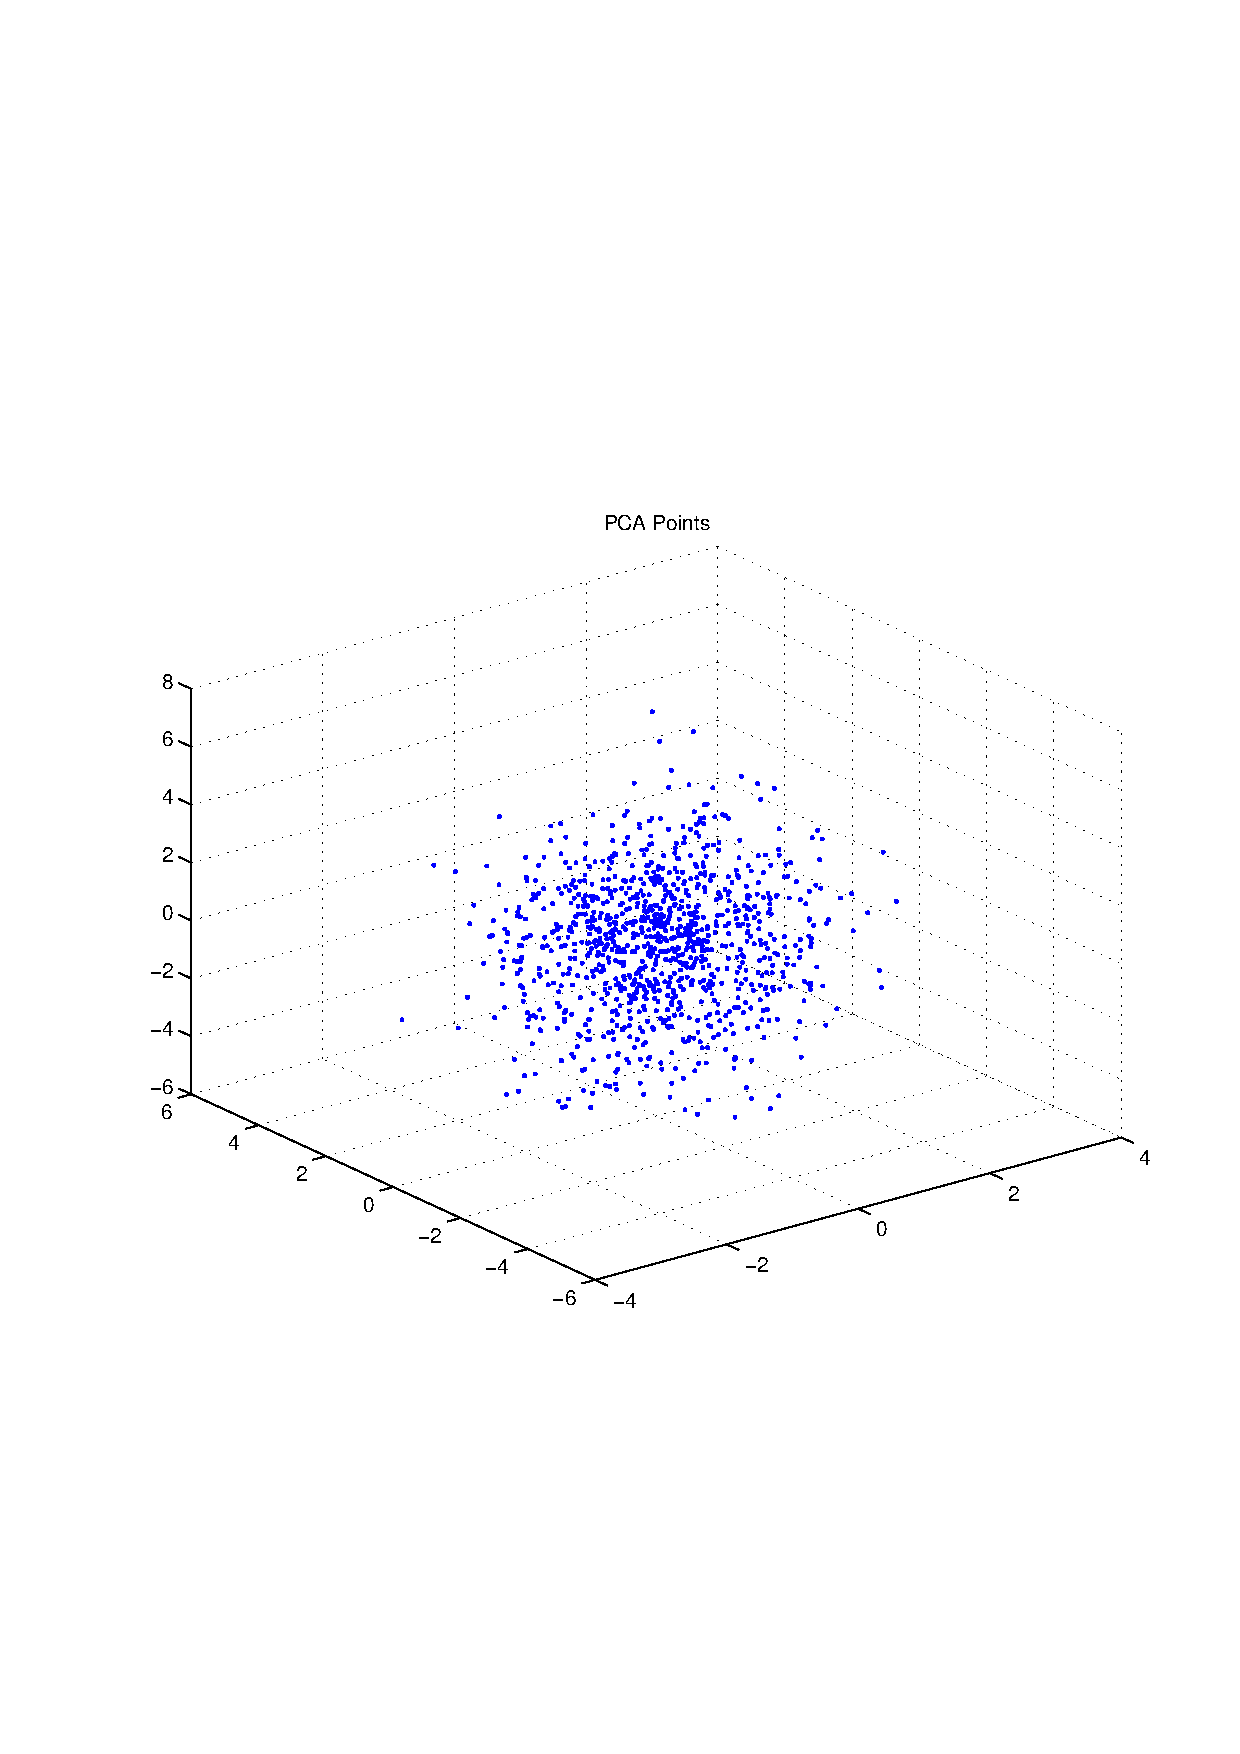
\includegraphics[width=10.0cm,height=10.0cm]{PCAPoints.pdf}

The eigenvectors:
+0.088, +0.196, +0.977
+0.199, +0.957, -0.210
-0.976, +0.213, +0.045

All of the eigenvalues of the covariance matrix:
(+0.958,+0.000), (+2.025,+0.000), (+3.017,+0.000)

QueryPerformanceCounter  =  +1.085
\subsubsection{Multi Variate Random Number Generator }
Sample from $N(\mu,\Sigma)$
mean= -0.002, variance=+1.004, skewness=+0.006, kurtosis=+3.003
mean= -0.001, variance=+1.017, skewness=-0.005, kurtosis=+2.988
mean= -0.002, variance=+1.006, skewness=-0.016, kurtosis=+3.014
Covariance Matrix 
+1.004, +0.009, +0.003
+0.009, +1.017, -0.003
+0.003, -0.003, +1.006

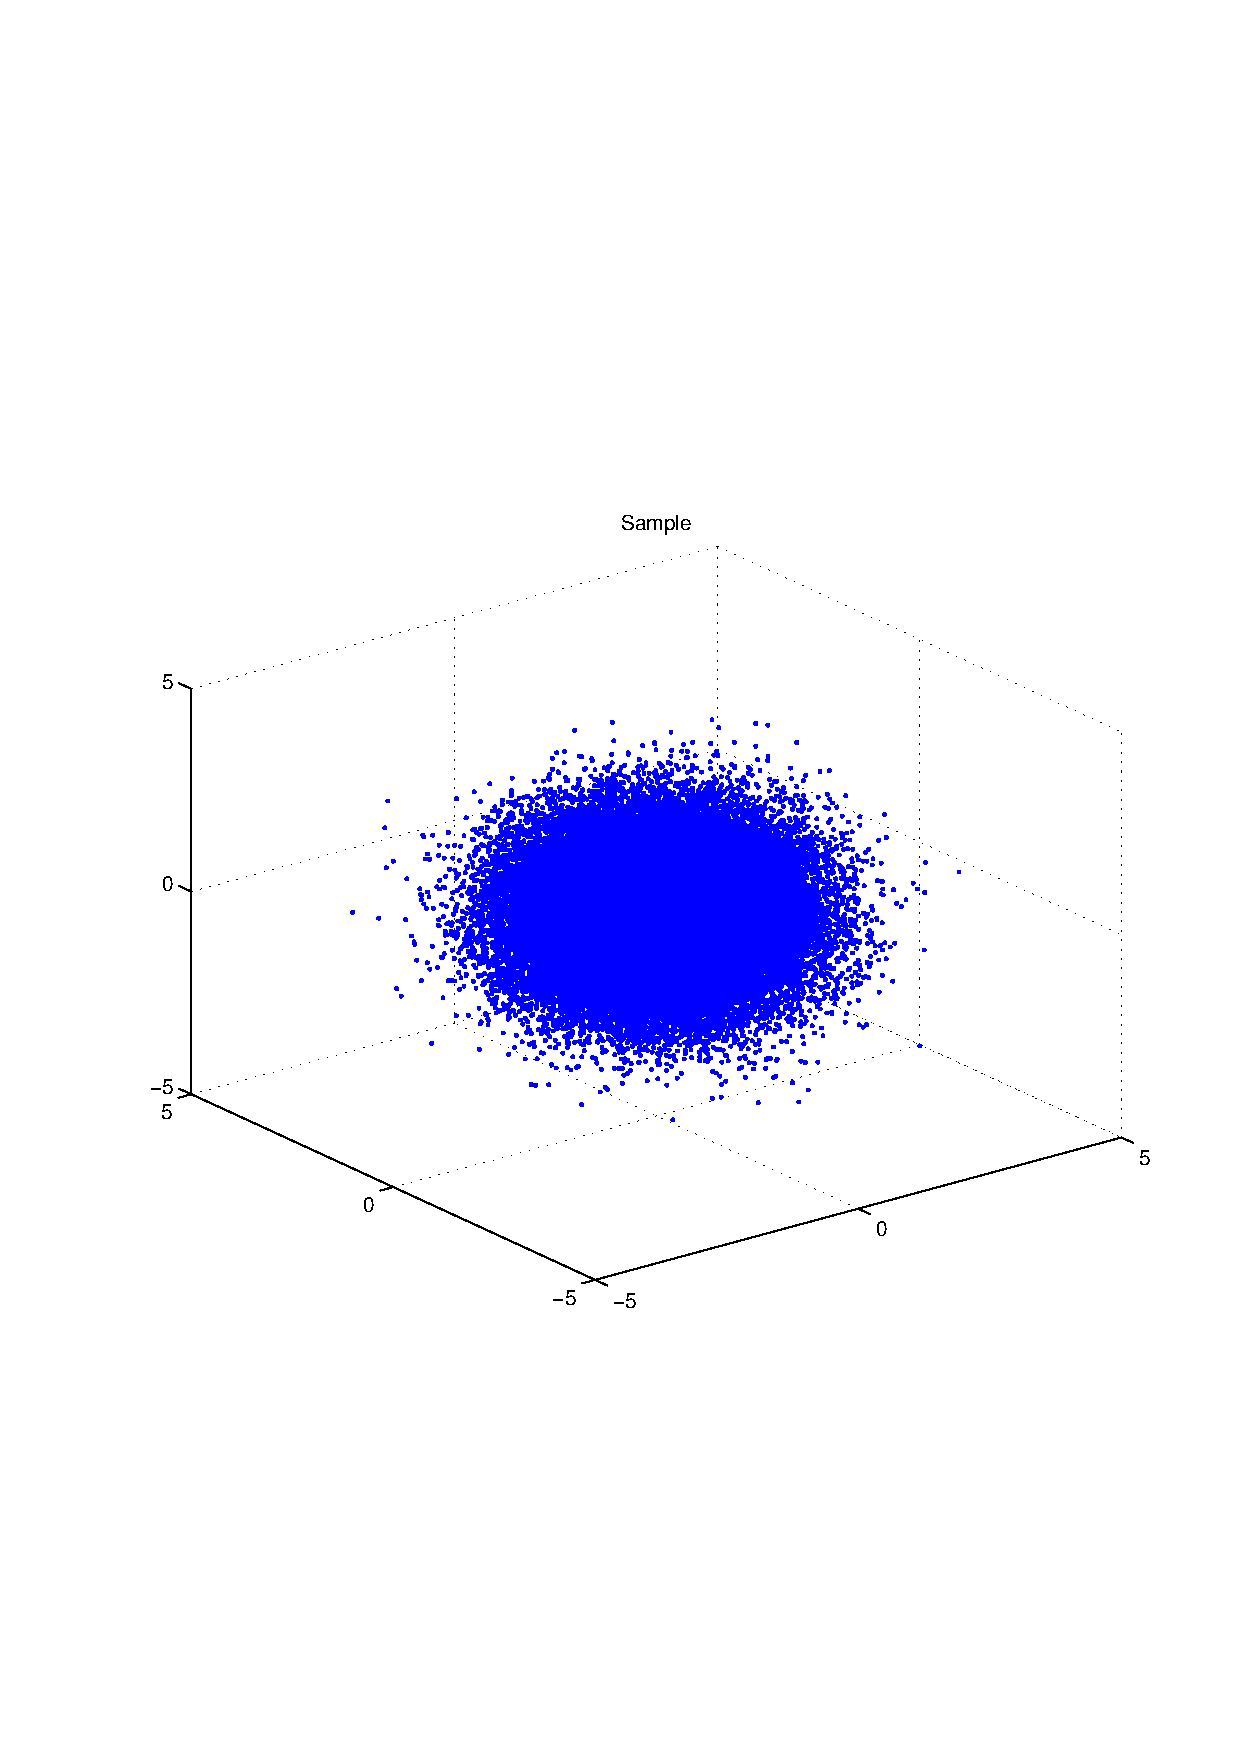
\includegraphics[width=10.0cm,height=10.0cm]{R_3_Normal.pdf}

Generate a sample from a unifom mixture of three Gaussians in $R^3$
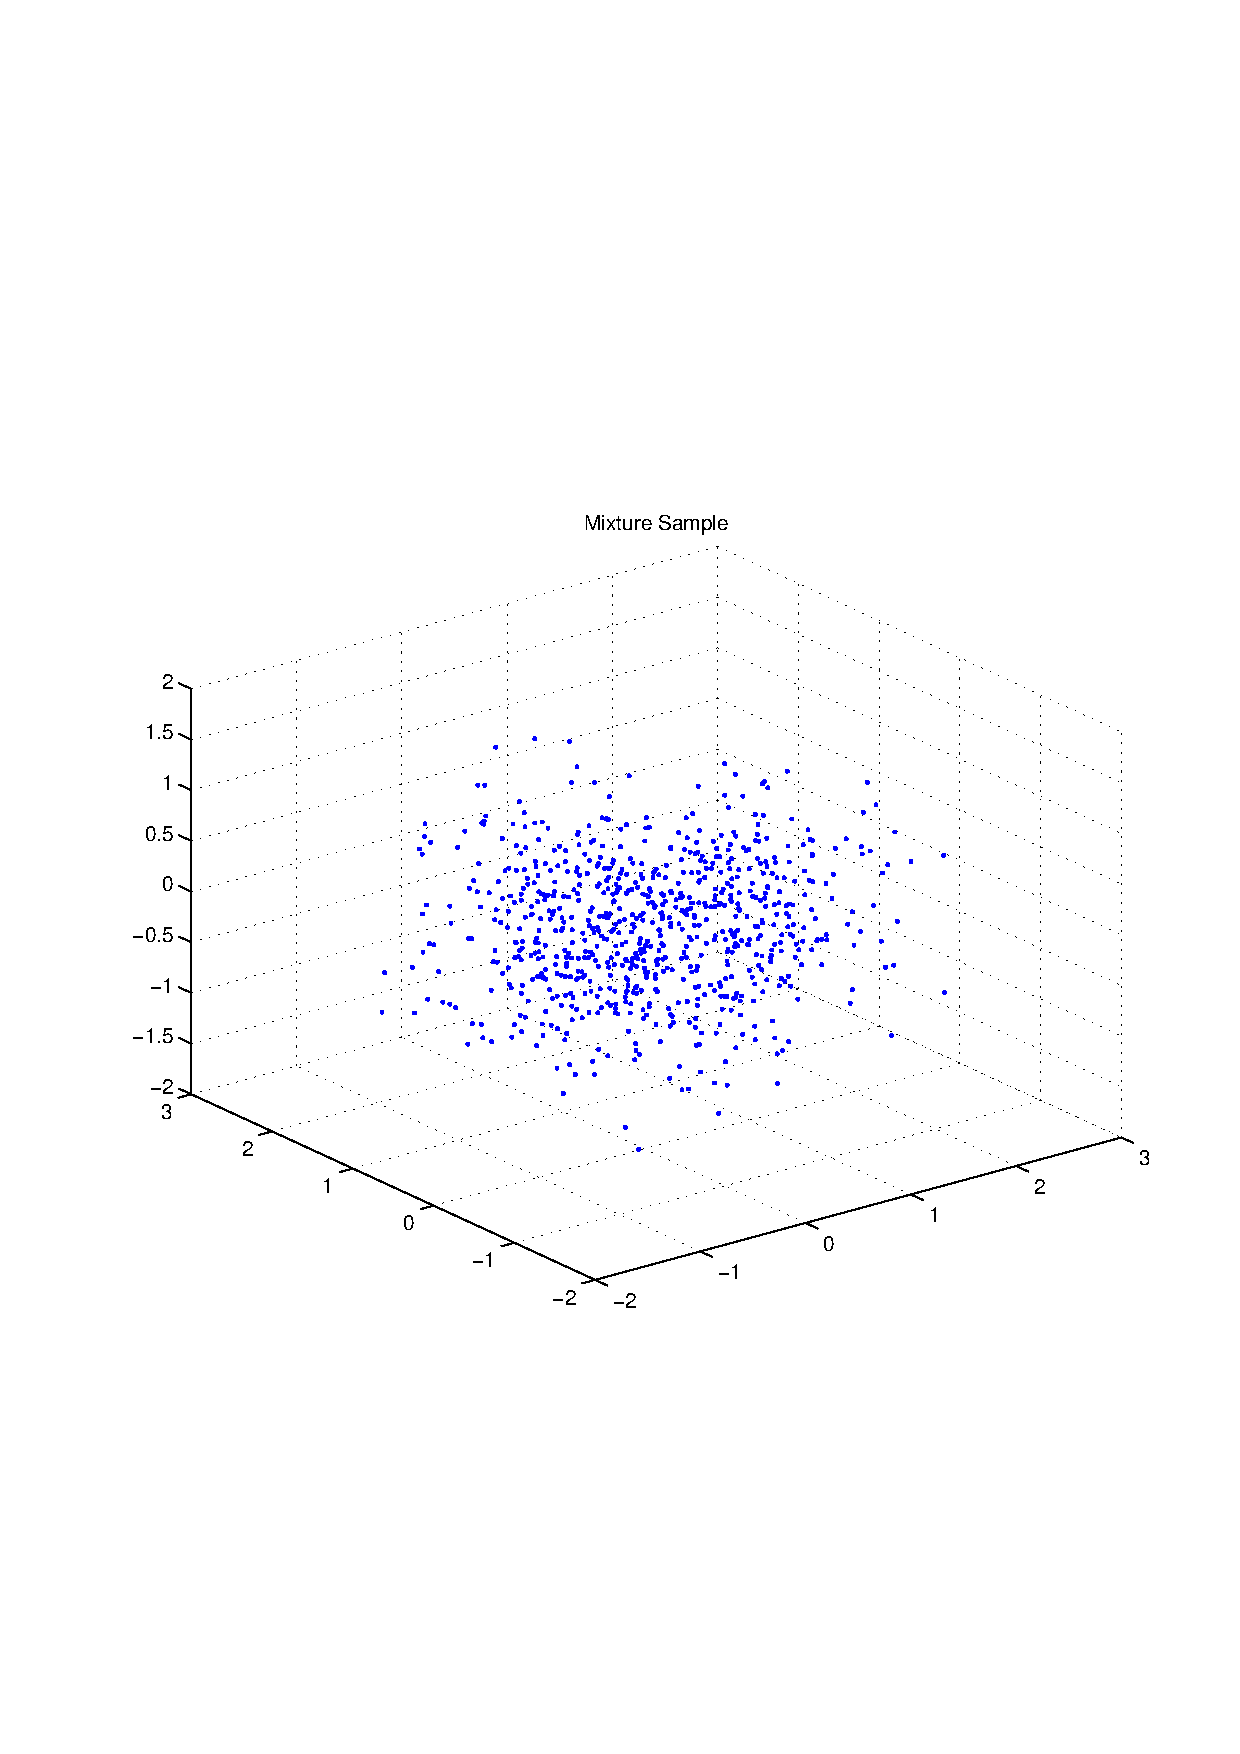
\includegraphics[width=10.0cm,height=10.0cm]{R_3_Normal_Mixture.pdf}

QueryPerformanceCounter  =  +16.555
\subsubsection{Matrix Multiply}
Comparing naive matrix multiply verus Intel MKL dgemm for matrix of size +2048.
This is for type double (hence the d in dgemm).
Naive type double matrix multiply tic toc  =  +0.346
dgemm plus row to column major transpose operation tic toc  =  +0.315
Comparing naive matrix multiply verus Intel MKL sgemm for matrix of size +2048.
This is for type float (hence the s in dgemm).
Naive type float matrix multiply tic toc  =  +0.239
sgemm plus row to column major transpose operation tic toc  =  +0.203
QueryPerformanceCounter  =  +1.234
\subsubsection{Descriptive Statistics}
Mean N(0,1): +0.003
Variance N(0,1): +1.006
Mean N(0,1) [recurrence relation method] :+0.003
Variance [recurrence relation method] :+1.006
Skewness : +0.007
Kurtosis : +2.997
QueryPerformanceCounter  =  +0.019
\subsubsection{Time Series }
+0.093
+0.726
+0.011
+2.178
QueryPerformanceCounter  =  +0.031
QueryPerformanceCounter  =  +5.802
\subsubsection{Iterated Exponential Filtering }
$\mu_1 =+0.093$
$\mu_2 =+0.726$
$\mu_3 =+0.011$
$\mu_4 =+2.178$
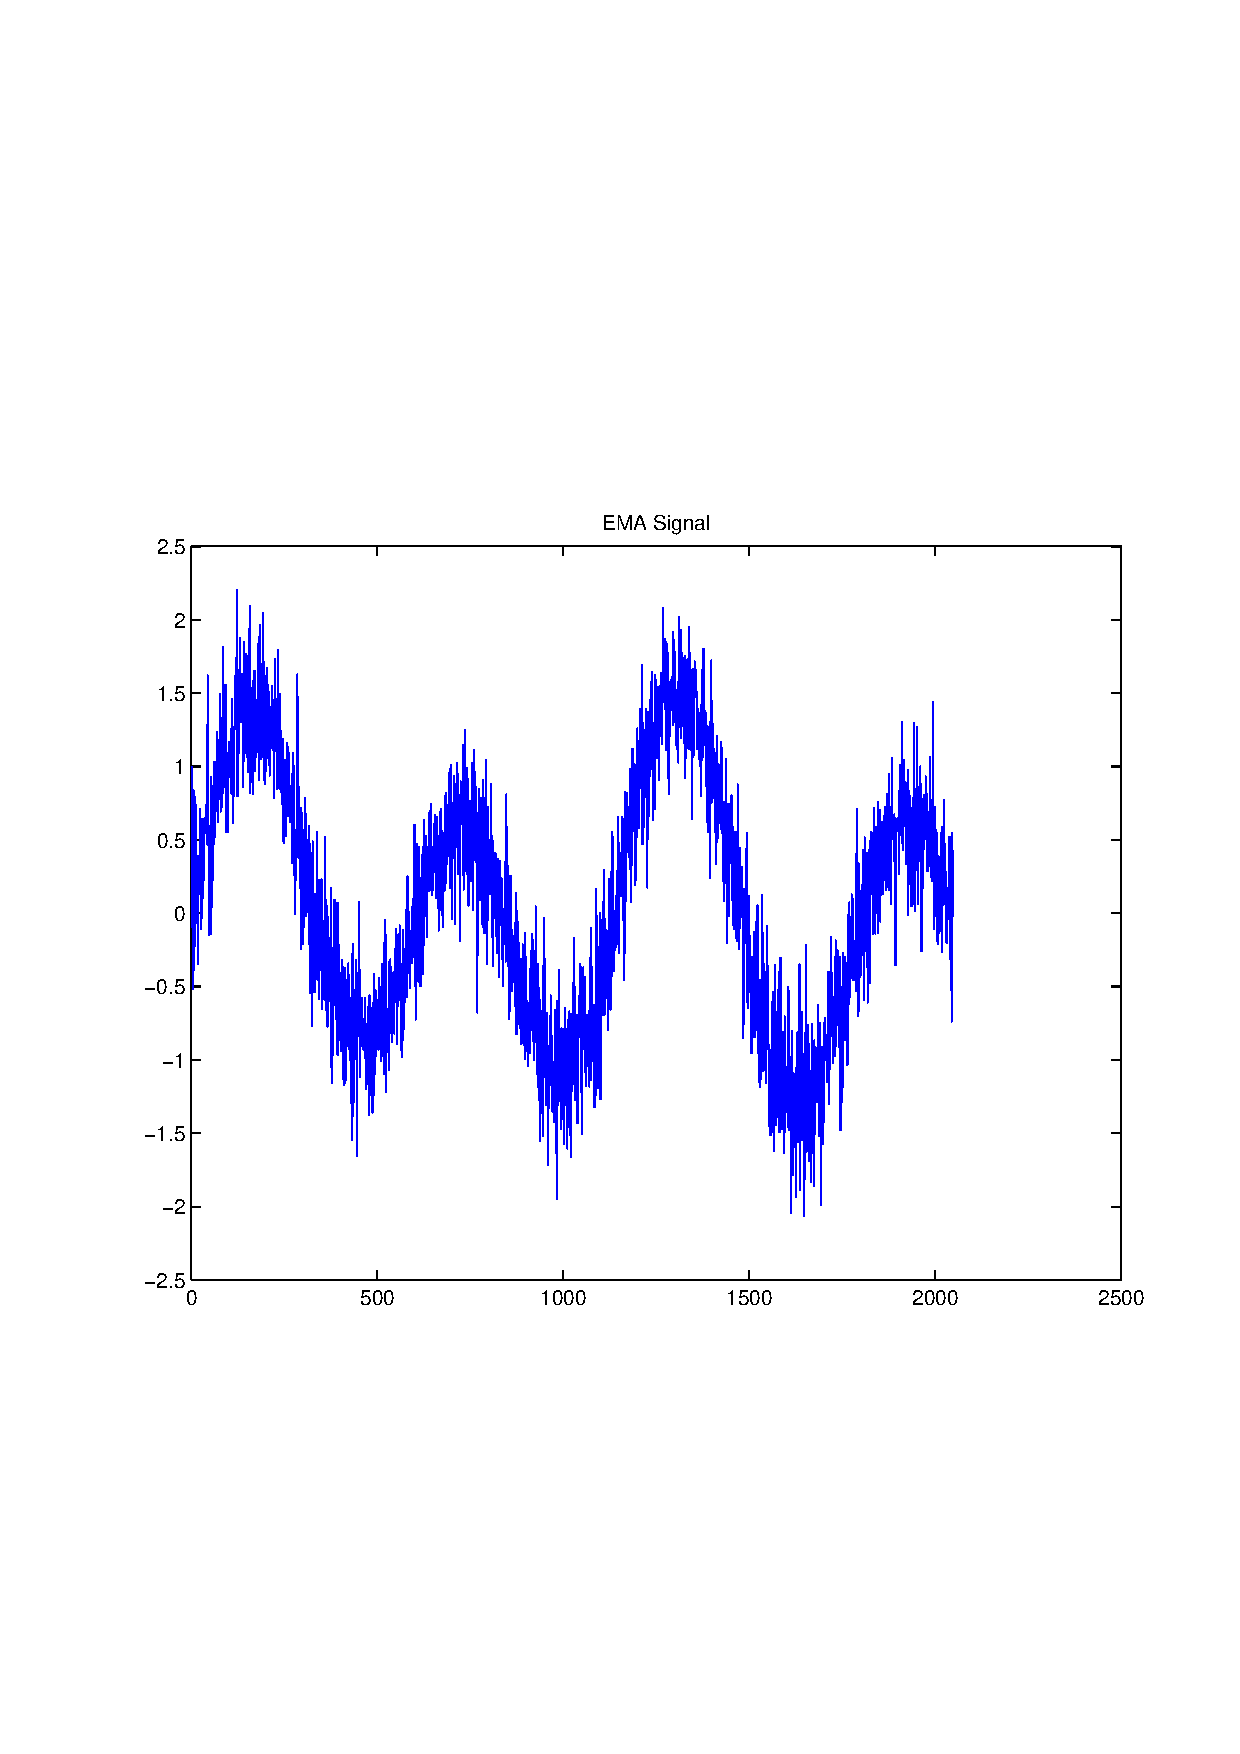
\includegraphics[width=10.0cm,height=10.0cm]{EMA_signal.pdf}

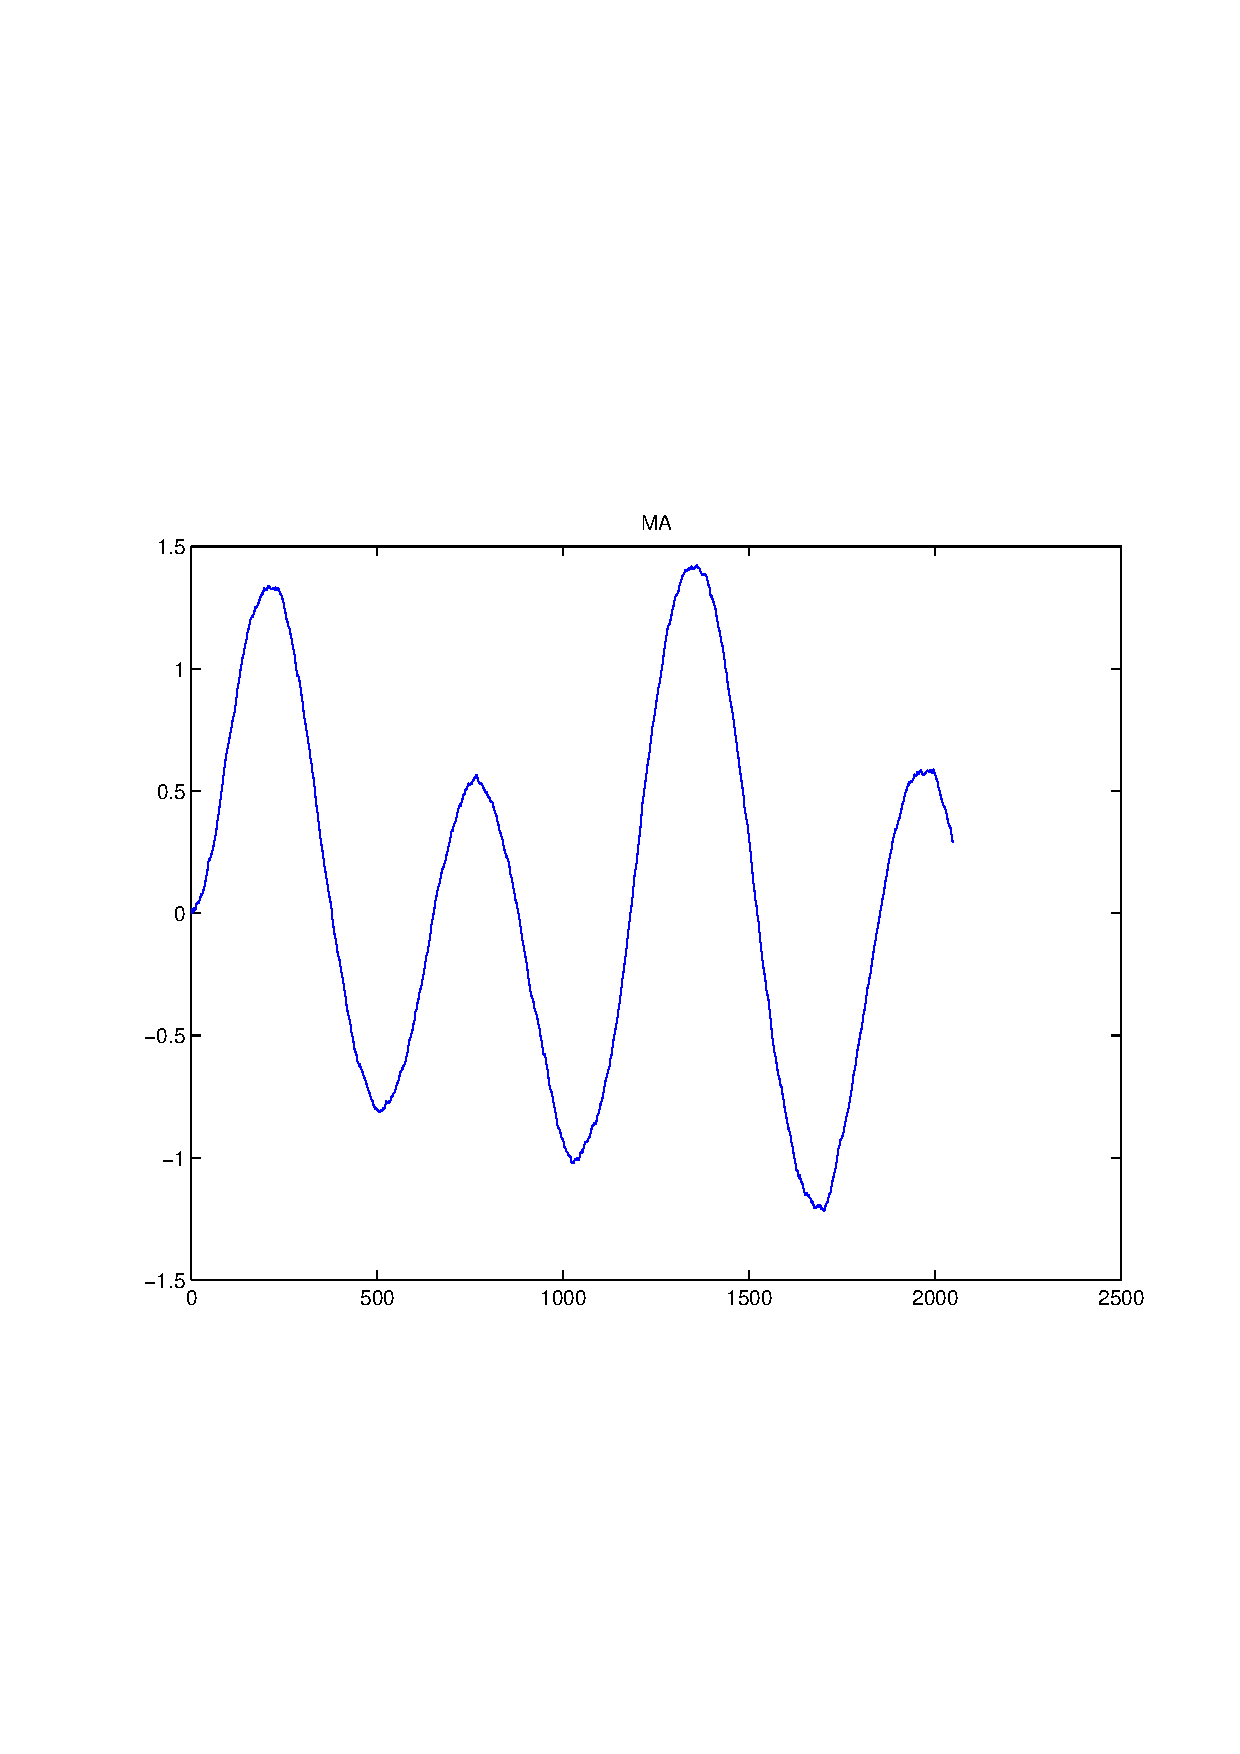
\includegraphics[width=10.0cm,height=10.0cm]{MA.pdf}

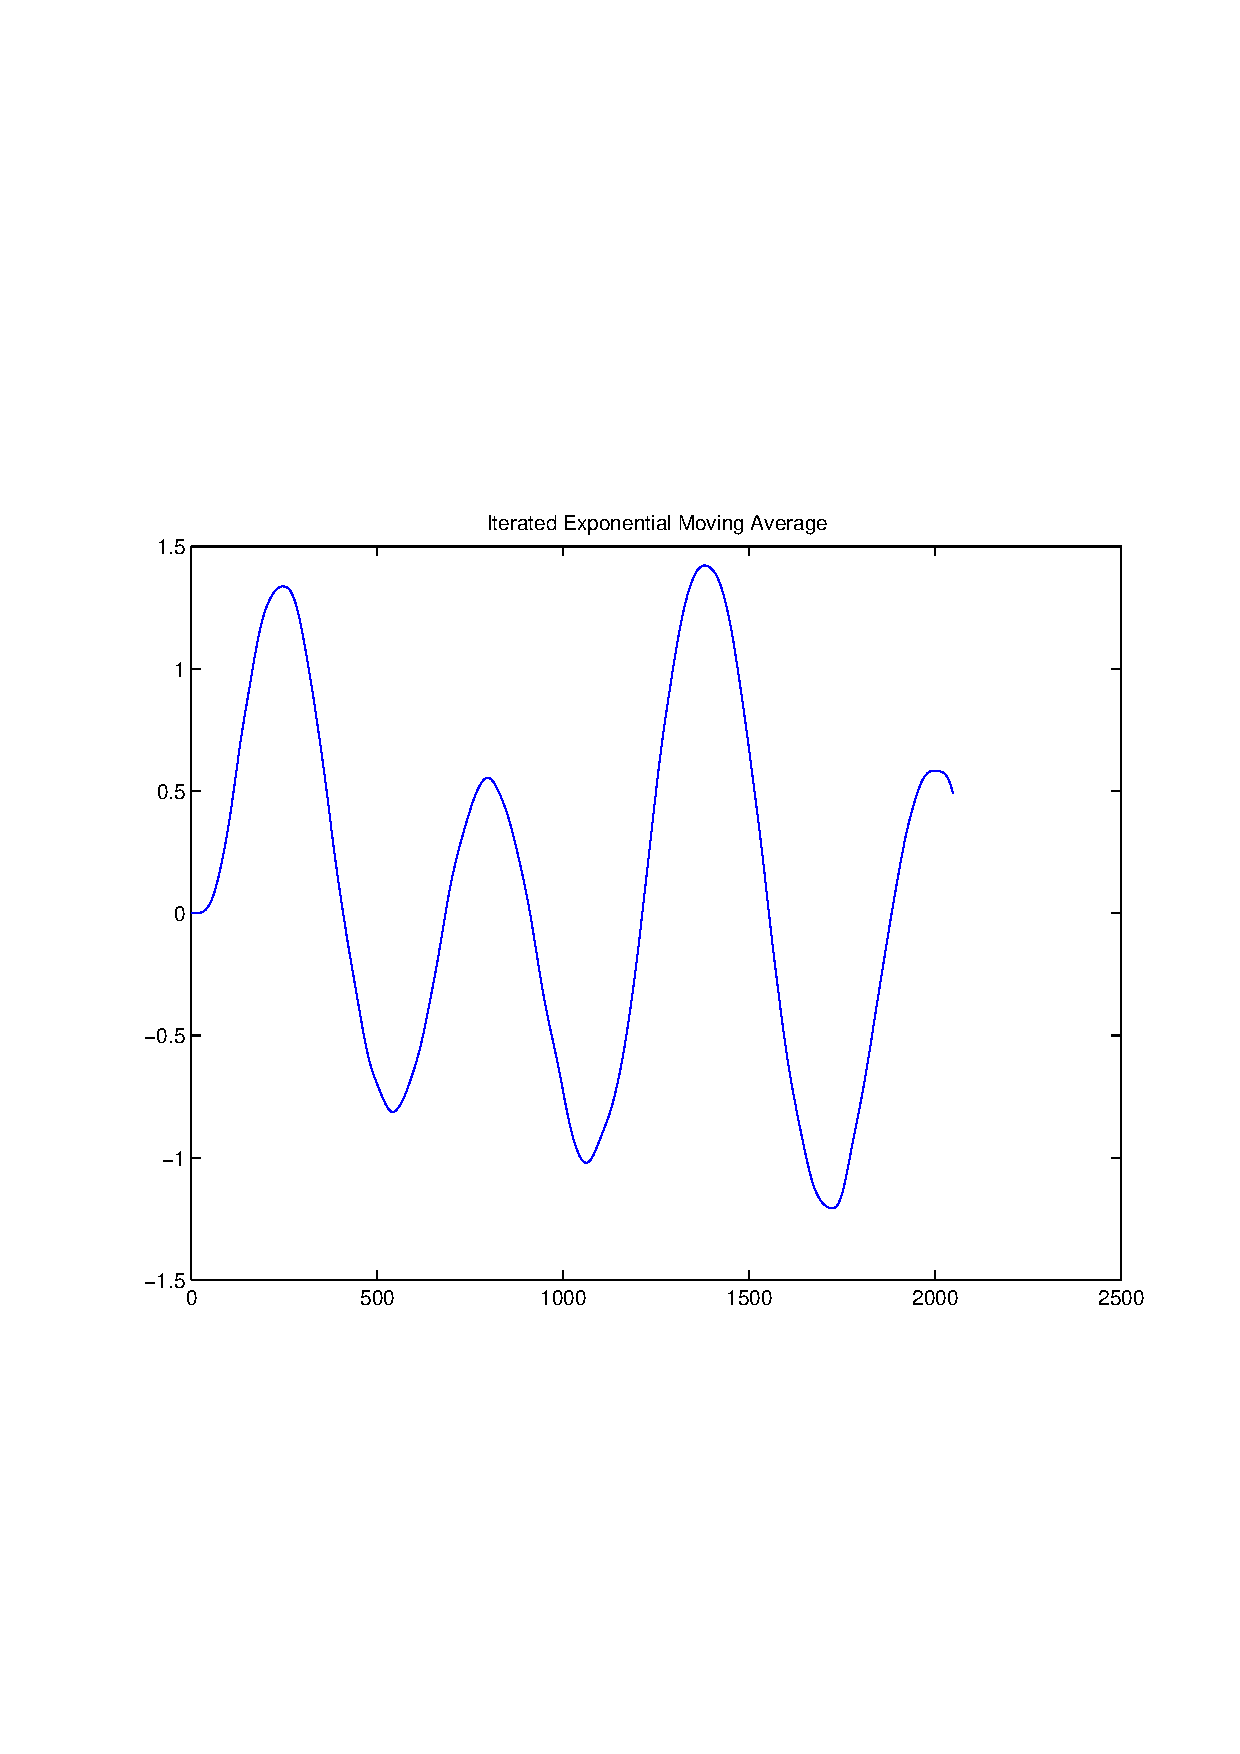
\includegraphics[width=10.0cm,height=10.0cm]{IEMA.pdf}

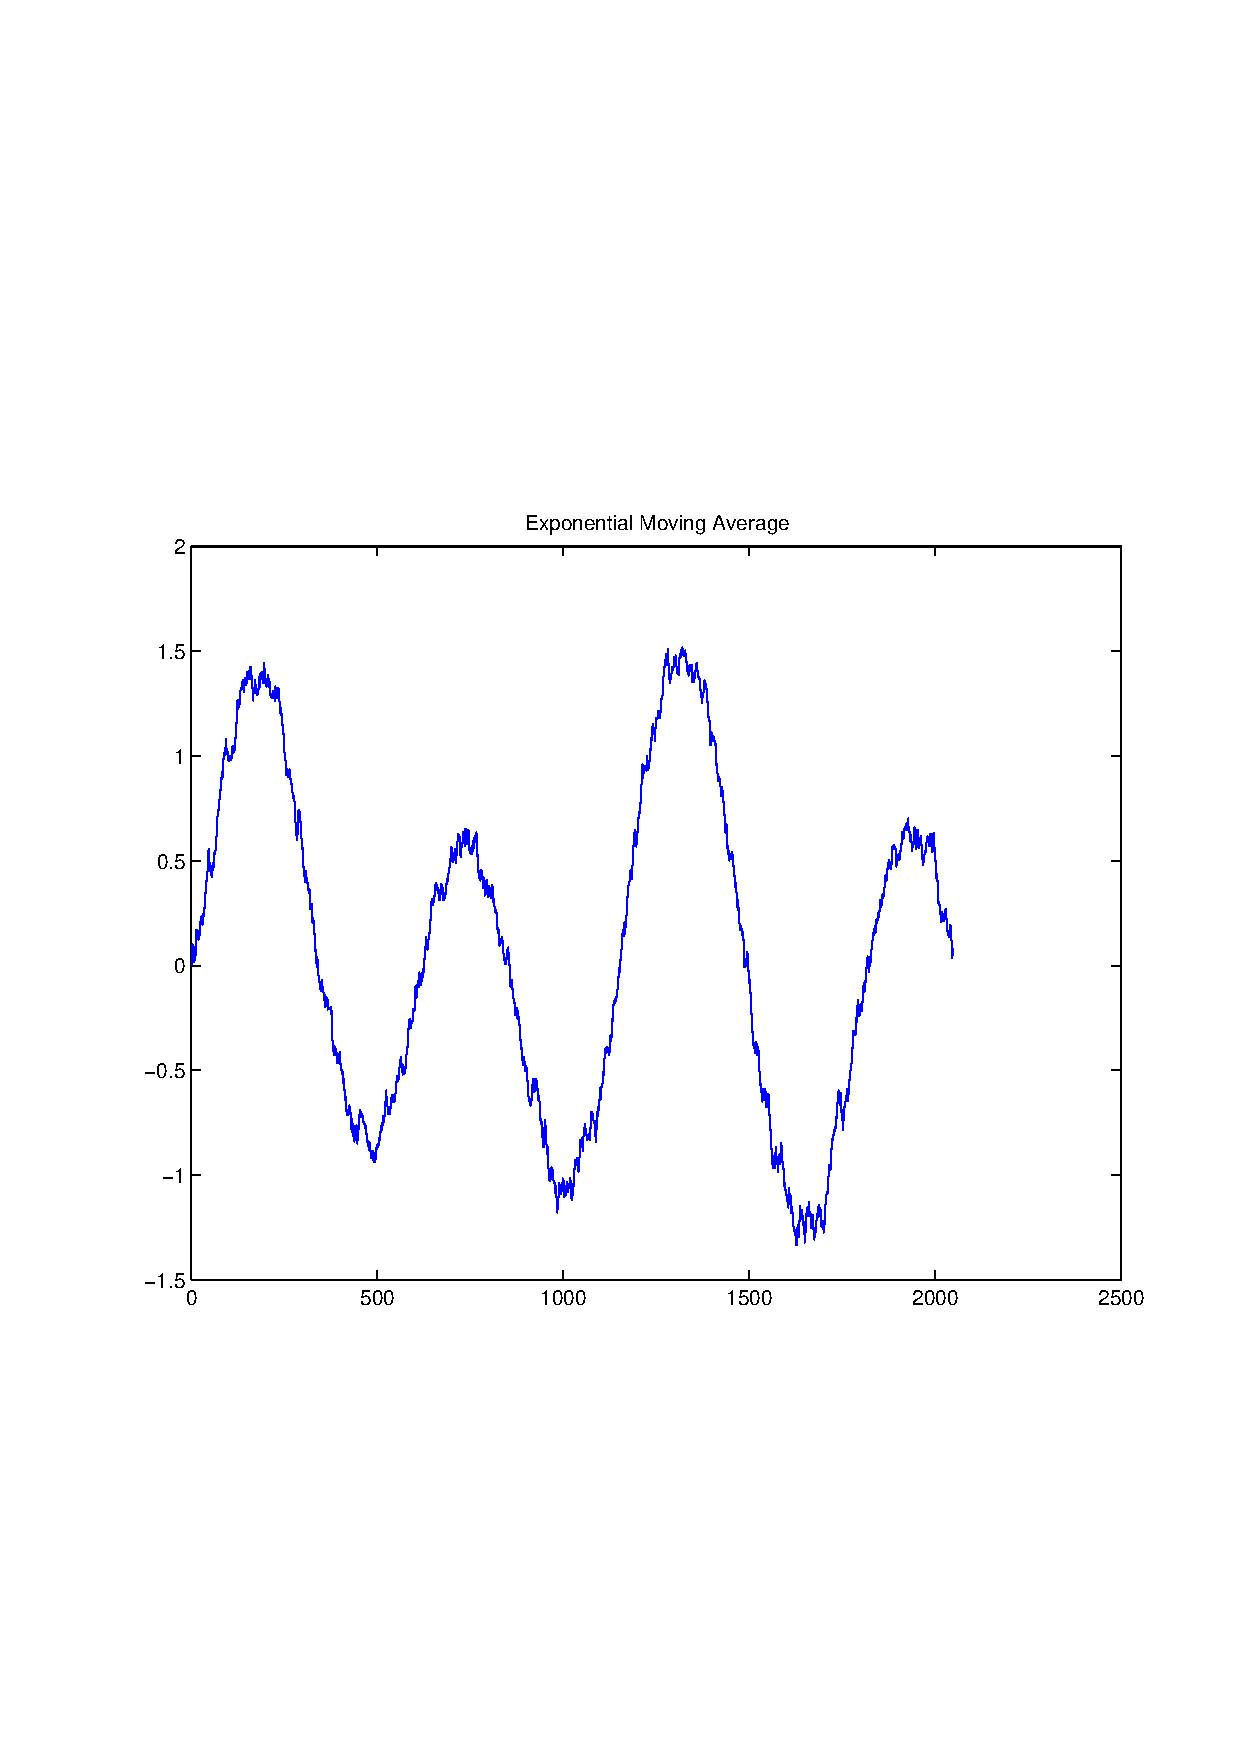
\includegraphics[width=10.0cm,height=10.0cm]{EMA.pdf}

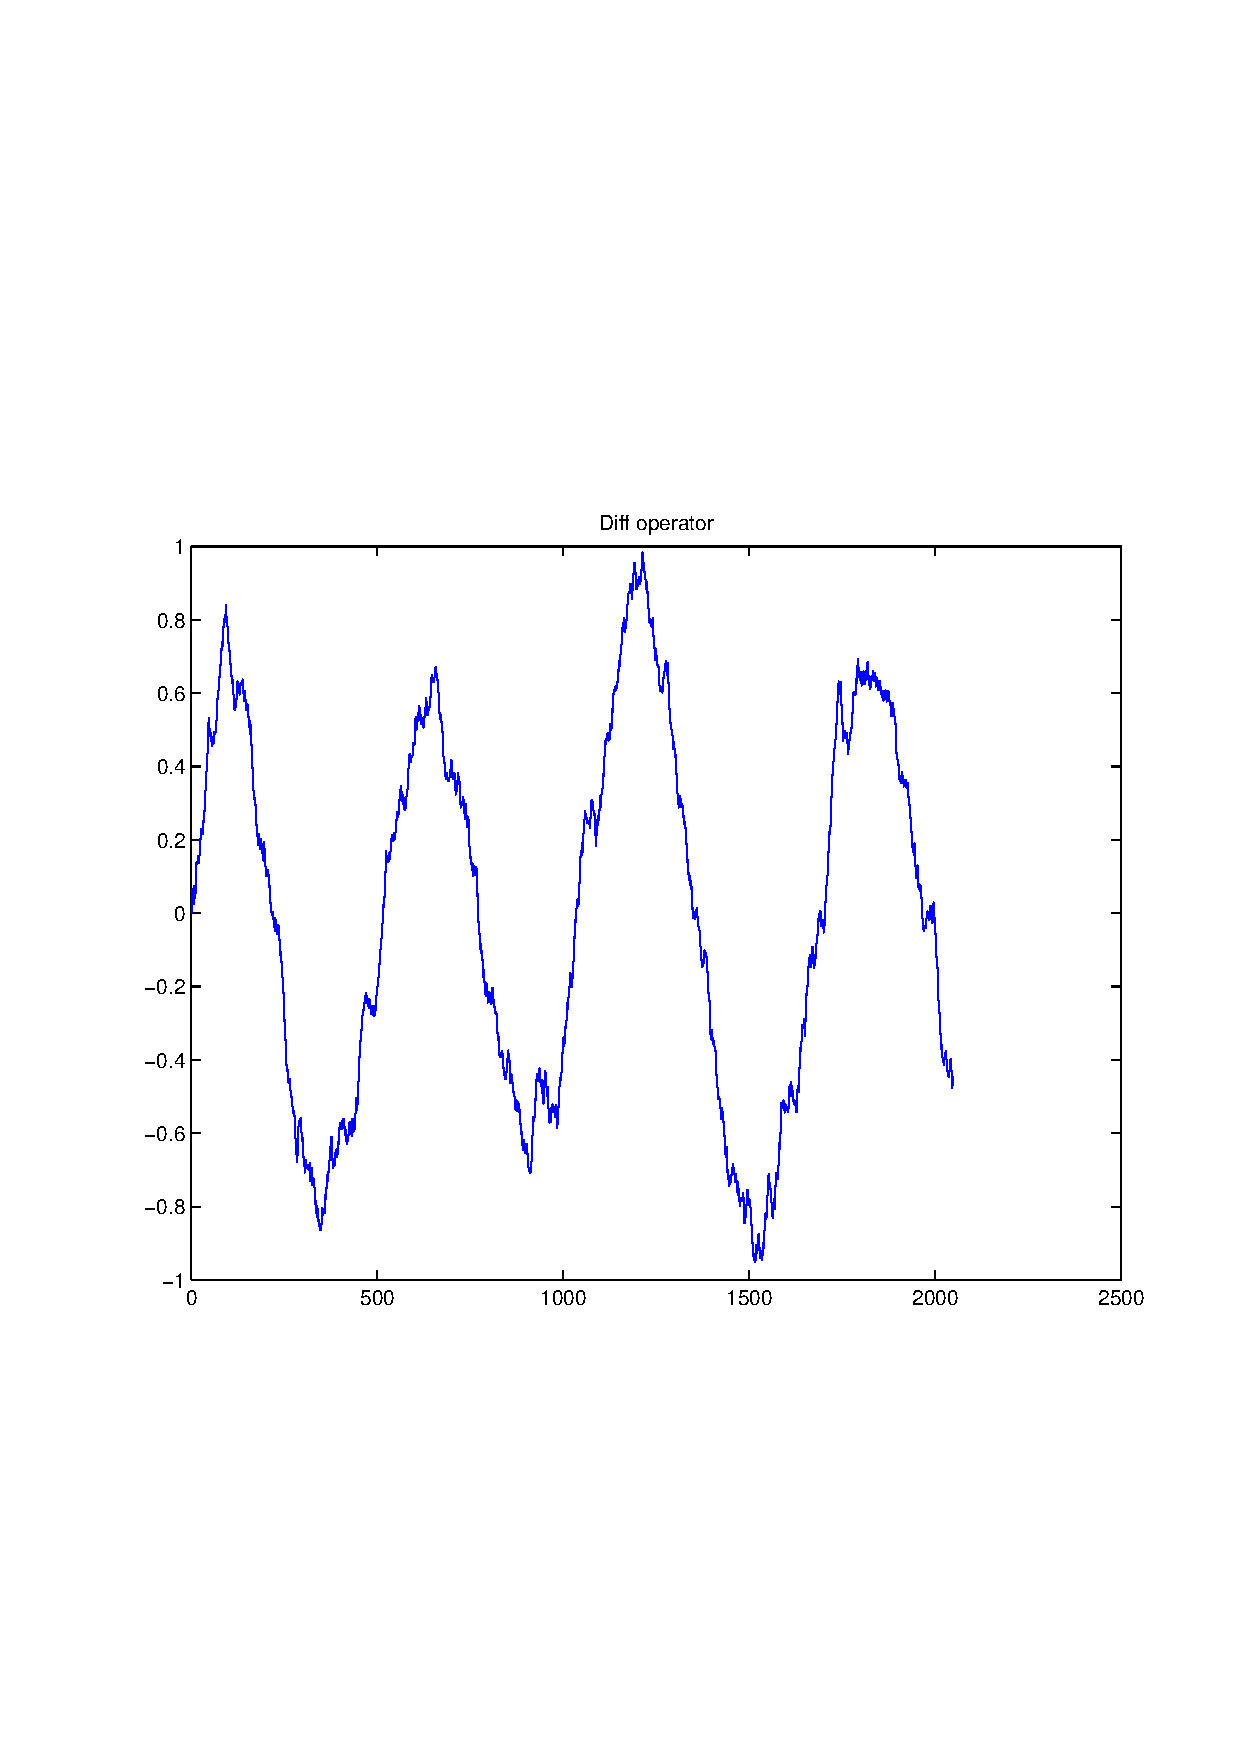
\includegraphics[width=10.0cm,height=10.0cm]{DIFF.pdf}

\includegraphics[width=10.0cm,height=10.0cm]{IteratedExponentailOperators.pdf}

\includegraphics[width=10.0cm,height=10.0cm]{IteratedExponentailOperators.pdf}

QueryPerformanceCounter  =  +7.981
\subsubsection{Testing binary writer}
Binary writer Speedup 1GB Double Matrix +49.810

Binary reader Speedup 1GB Double Matrix +188.774

Binary writer Speedup 1GB Double vector +11.364

Binary reader Speedup 1GB Double Matrix +135.811

QueryPerformanceCounter  =  +0.819
\subsubsection{Testing Gaussian Mixture Point Cloud and Latex Plotting Capabilities.}
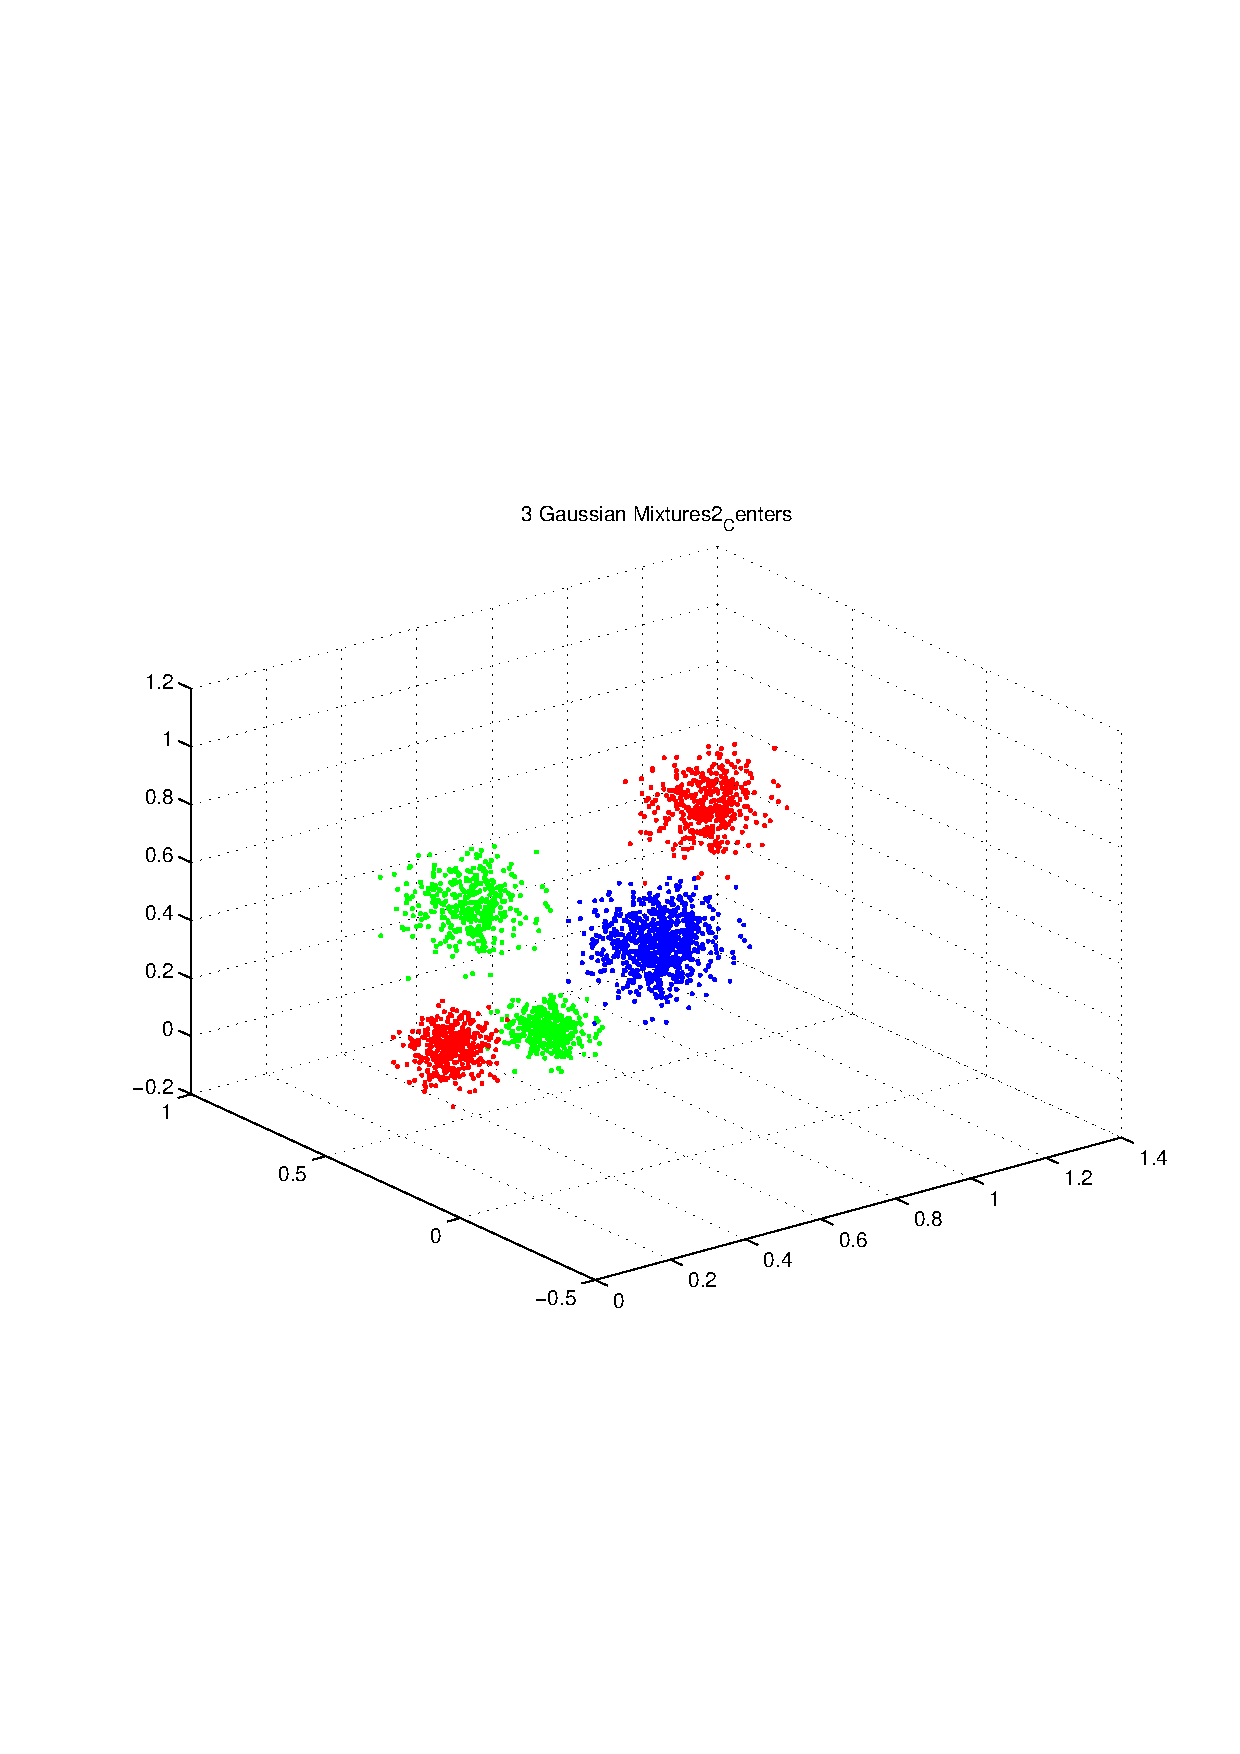
\includegraphics[width=10.0cm,height=10.0cm]{GaussianMixture_Dim_3_Centers2.pdf}

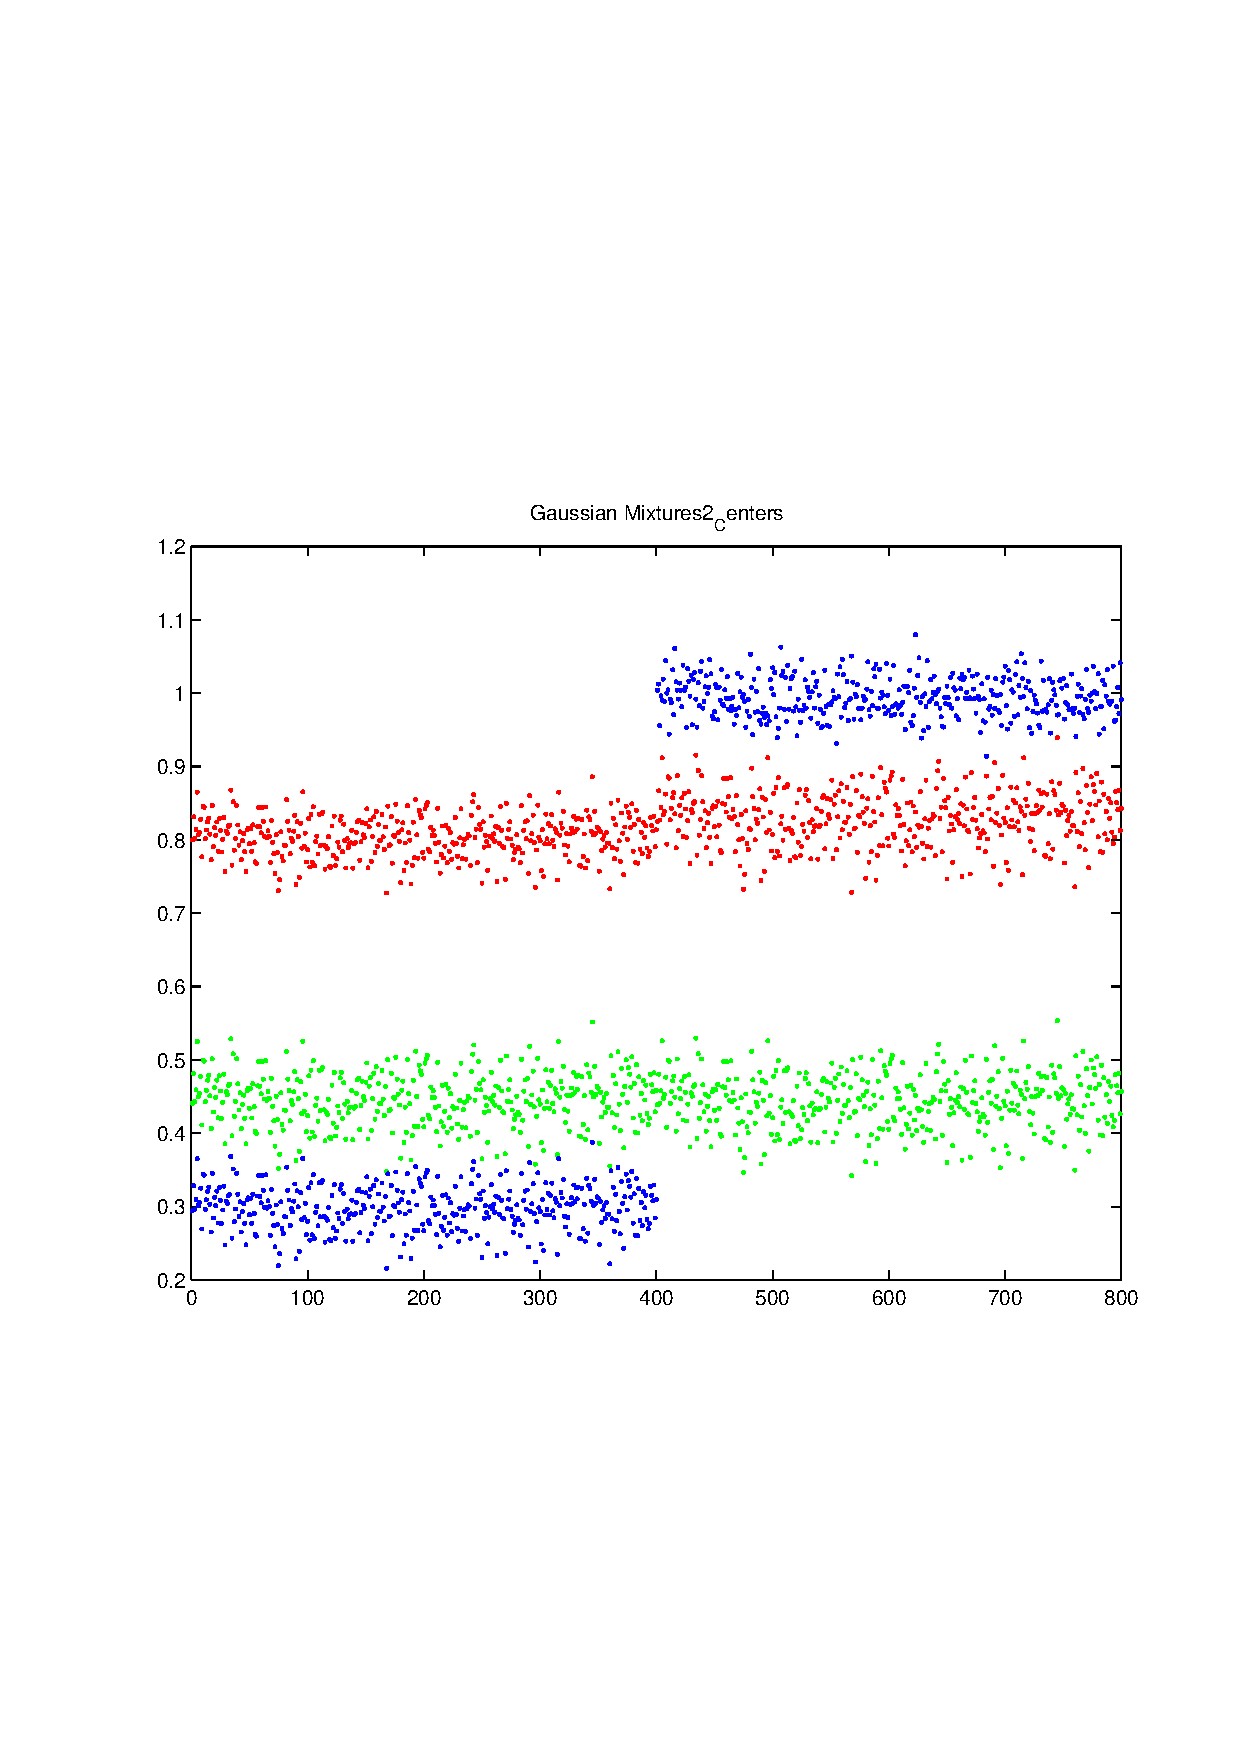
\includegraphics[width=10.0cm,height=10.0cm]{GaussianMixture_Dim_1_Centers2.pdf}

QueryPerformanceCounter  =  +2.926
\subsubsection{Intel VSL Function Check}
\includegraphics[width=10.0cm,height=10.0cm]{klVSLInv.pdf}

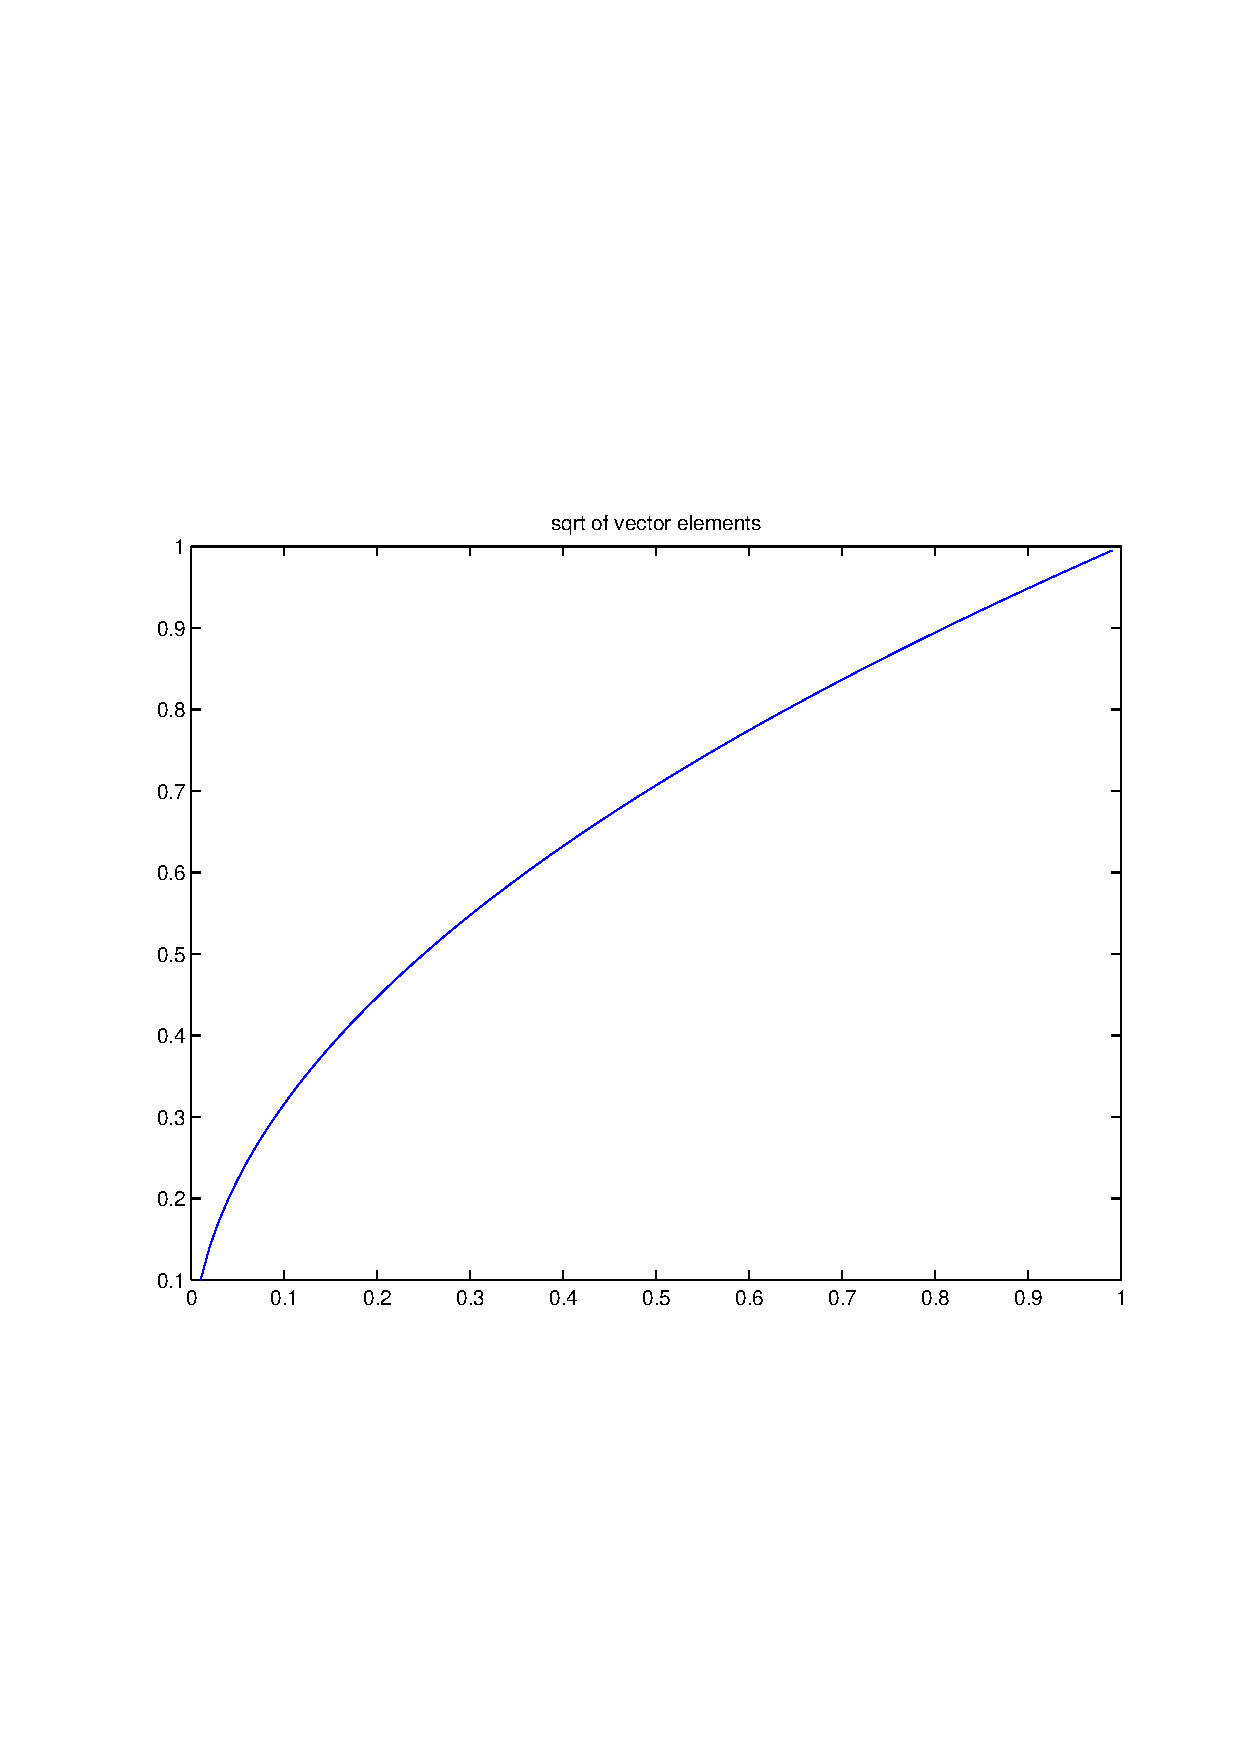
\includegraphics[width=10.0cm,height=10.0cm]{klVSLSqrt.pdf}

\includegraphics[width=10.0cm,height=10.0cm]{klVSLExp.pdf}

\includegraphics[width=10.0cm,height=10.0cm]{klVSLExpm1.pdf}

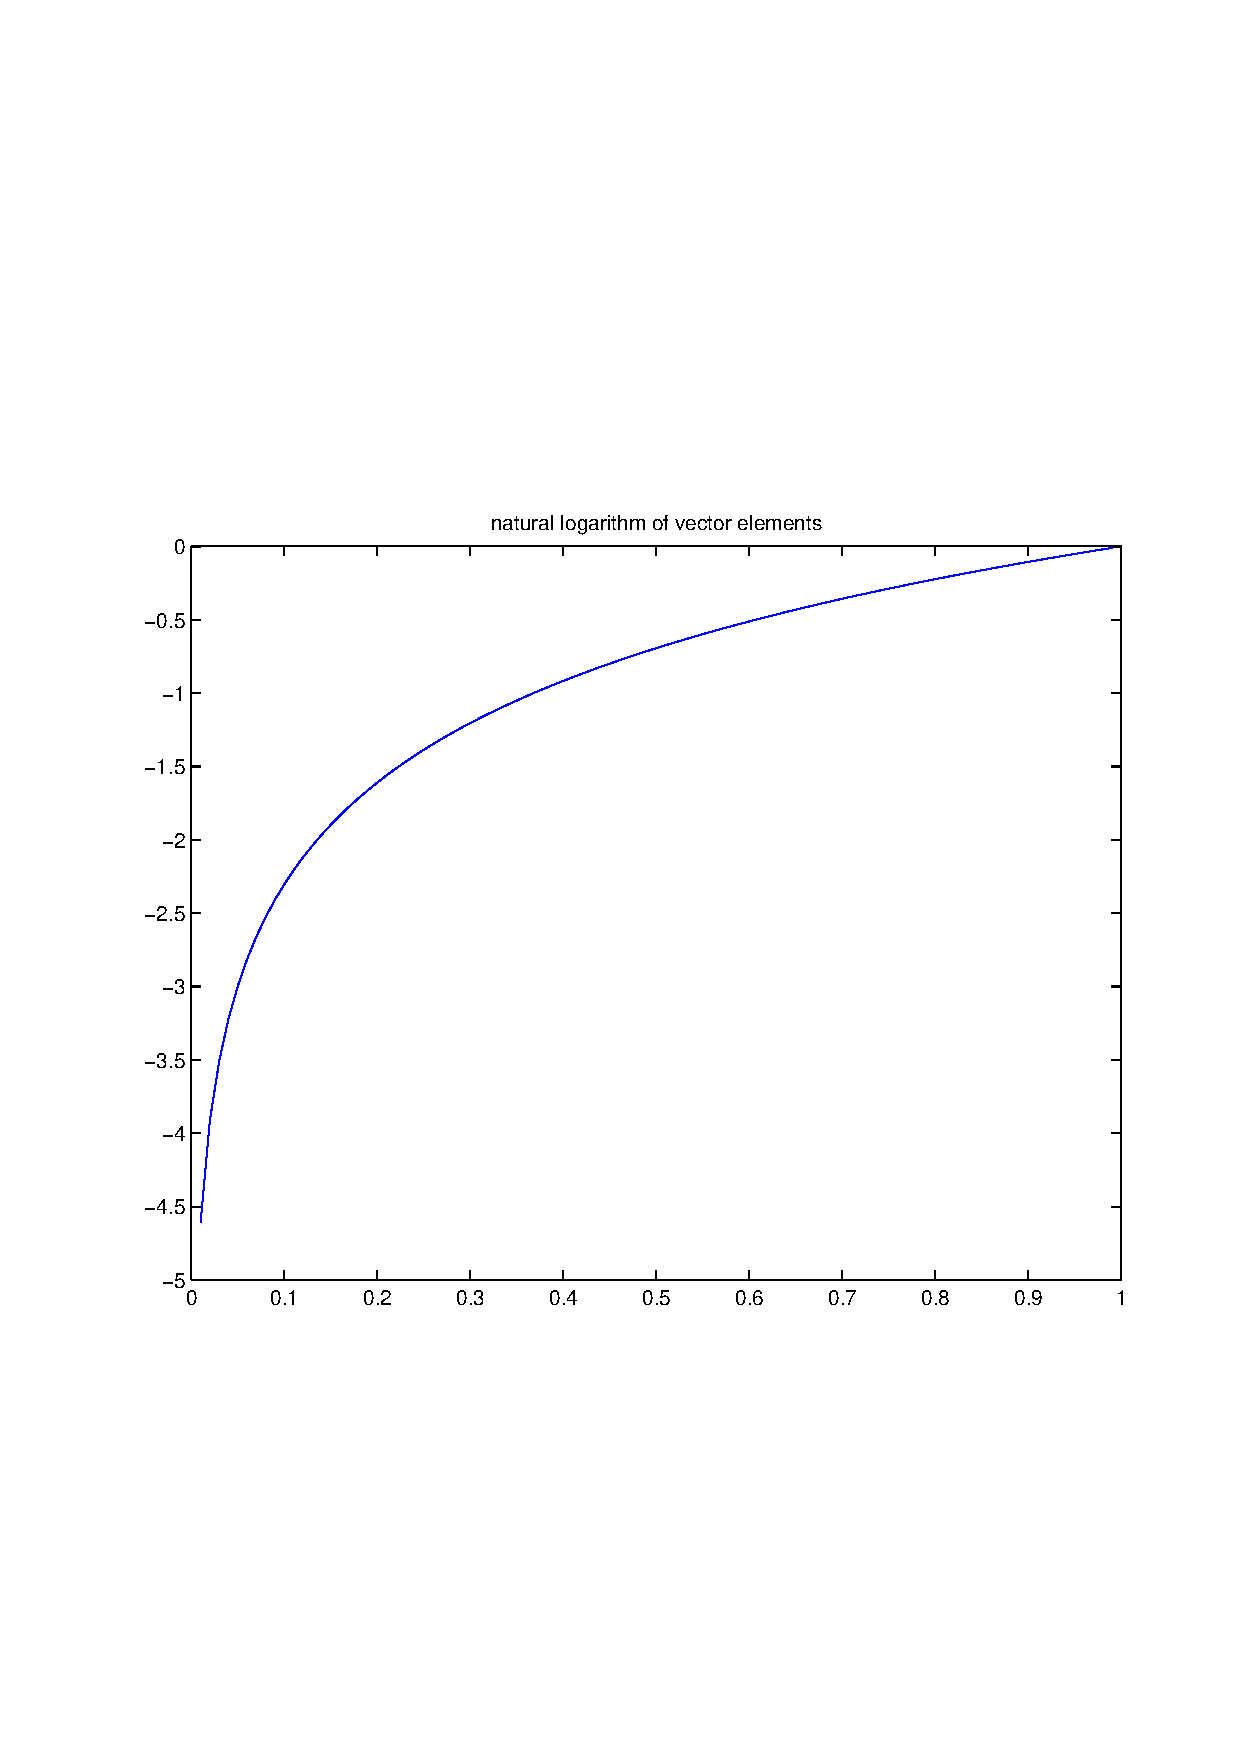
\includegraphics[width=10.0cm,height=10.0cm]{klVSLLn.pdf}

\includegraphics[width=10.0cm,height=10.0cm]{klVSLLog10.pdf}

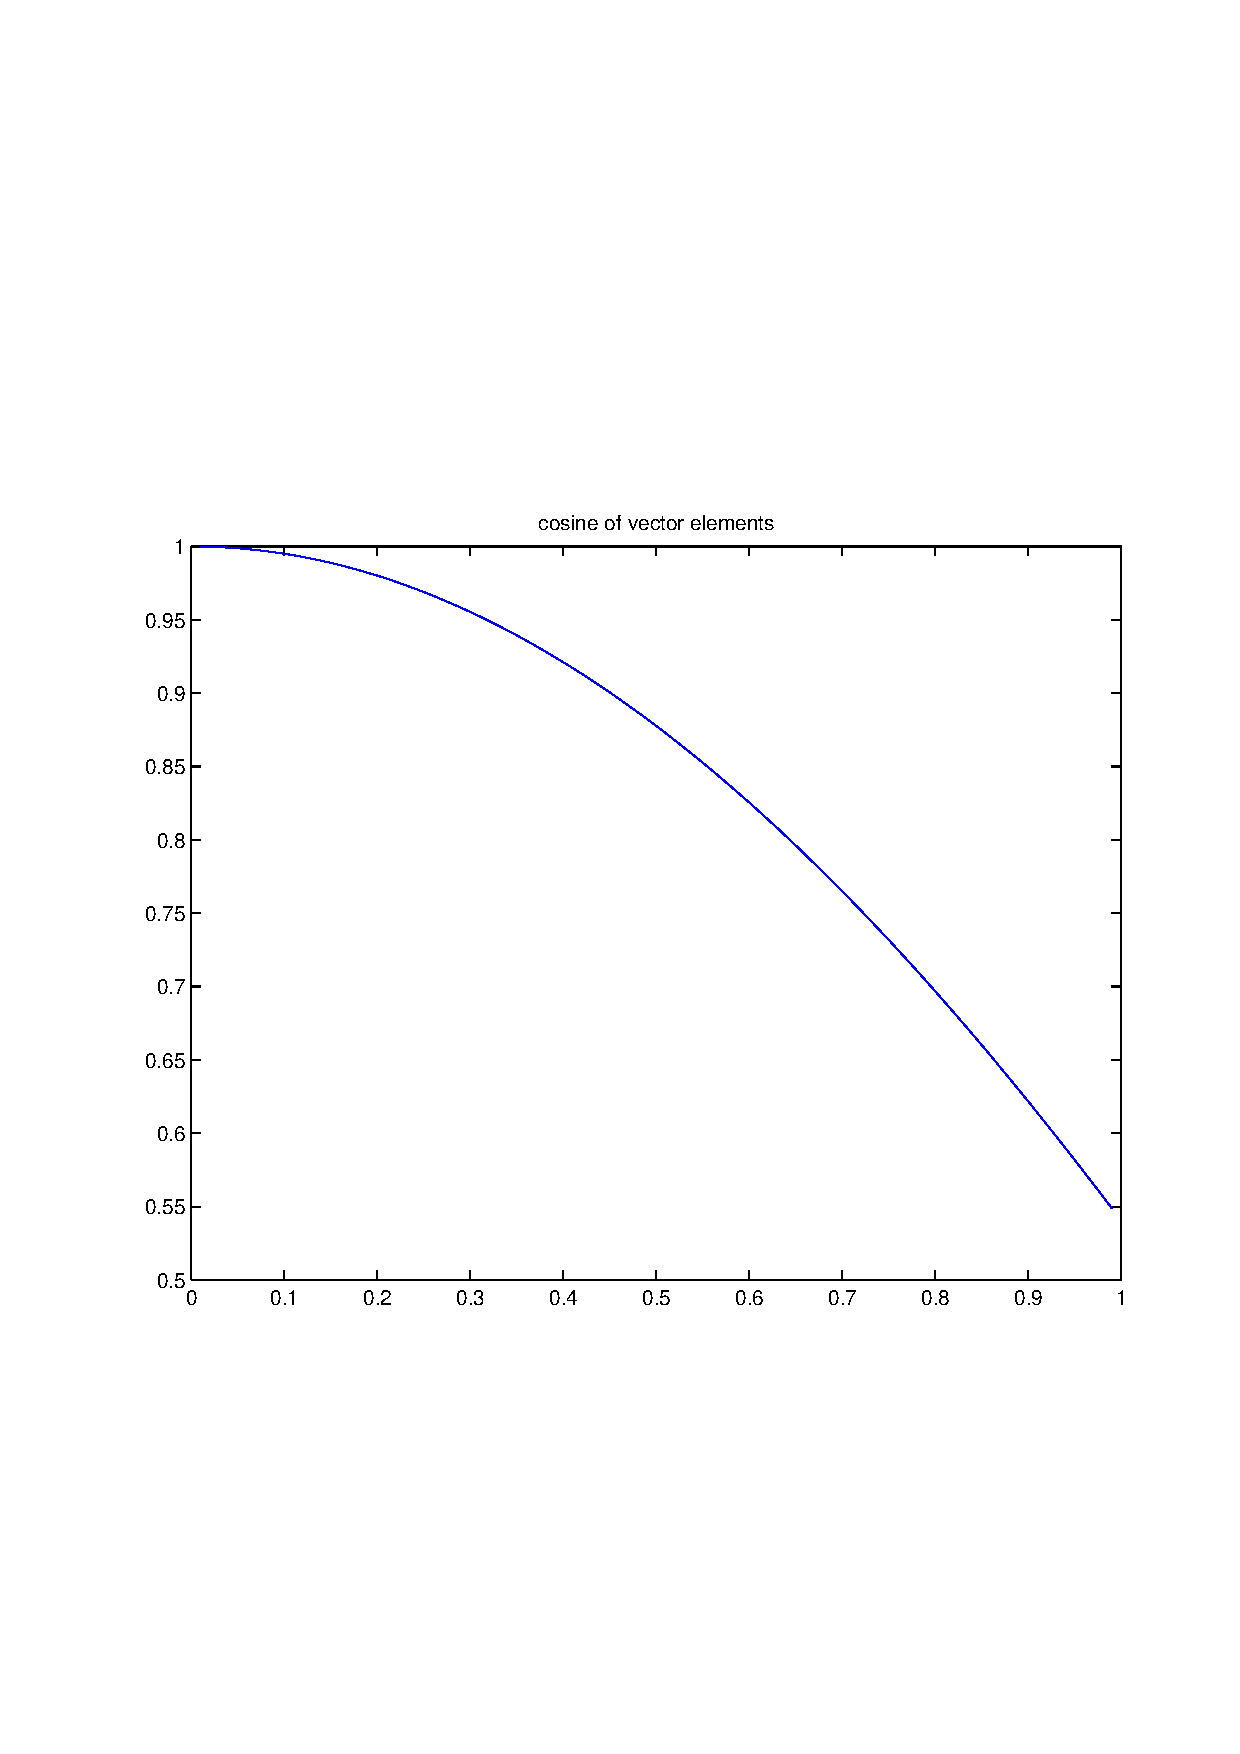
\includegraphics[width=10.0cm,height=10.0cm]{klVSLCos.pdf}

\includegraphics[width=10.0cm,height=10.0cm]{klVSLSin.pdf}

\includegraphics[width=10.0cm,height=10.0cm]{klVSLTan.pdf}

\includegraphics[width=10.0cm,height=10.0cm]{klVSLErf.pdf}

\includegraphics[width=10.0cm,height=10.0cm]{klVSLErfc.pdf}

\includegraphics[width=10.0cm,height=10.0cm]{klVSLCdfNorm.pdf}

\includegraphics[width=10.0cm,height=10.0cm]{klVSLErfInv.pdf}

\includegraphics[width=10.0cm,height=10.0cm]{klVSLLGamma.pdf}

\includegraphics[width=10.0cm,height=10.0cm]{klVSLTGamma.pdf}

QueryPerformanceCounter  =  +15.930
\subsubsection{Gram Matrix Consistency Check}
Sample Size = 4096
Feature dim = 3

$$Sigma$ = \left(
\begin{array}{
ccc}
+1.140 & +1.535 & +0.581 \\
+1.535 & +9.988 & +1.605 \\
+0.581 & +1.605 & +0.428 \\
\end{array}
\right)$ \newline 

$Sample Covariance = \left(
\begin{array}{
ccc}
+1.145 & +1.558 & +0.589 \\
+1.558 & +9.859 & +1.631 \\
+0.589 & +1.631 & +0.438 \\
\end{array}
\right)$ \newline 

$Sample Mean = \left(
\begin{array}{
ccc}
+1.02837 & +1.08592 & +1.01901 \\
\end{array}
\right)$ \newline 

$Sample Covariance-$Omega$ = \left(
\begin{array}{
ccc}
+0.006 & +0.022 & +0.008 \\
+0.022 & -0.129 & +0.025 \\
+0.008 & +0.025 & +0.011 \\
\end{array}
\right)$ \newline 

$Sample Covariance Eigs = \left(
\begin{array}{
ccc}
(+10.42140,+0.00000) & (+0.98121,+0.00000) & (+0.04033,+0.00000) \\
\end{array}
\right)$ \newline 

$Centered Mean = \left(
\begin{array}{
ccc}
+0.00000 & -0.00000 & +0.00000 \\
\end{array}
\right)$ \newline 

$Centered Covariance = \left(
\begin{array}{
ccc}
+1.145 & +1.558 & +0.589 \\
+1.558 & +9.859 & +1.631 \\
+0.589 & +1.631 & +0.438 \\
\end{array}
\right)$ \newline 

$Gram Matrix Gf Not scaled by sample size = \left(
\begin{array}{
ccc}
+4691.798 & +6378.015 & +2412.183 \\
+6378.015 & +40383.068 & +6677.072 \\
+2412.183 & +6677.072 & +1795.407 \\
\end{array}
\right)$ \newline 

$Gram Matrix Gf  scaled by sample size = \left(
\begin{array}{
ccc}
+1.145 & +1.557 & +0.589 \\
+1.557 & +9.859 & +1.630 \\
+0.589 & +1.630 & +0.438 \\
\end{array}
\right)$ \newline 

$SampleCovariance - Scaled Gf = \left(
\begin{array}{
ccc}
+0.000 & +0.000 & +0.000 \\
+0.000 & +0.002 & +0.000 \\
+0.000 & +0.000 & +0.000 \\
\end{array}
\right)$ \newline 

$EigenDecomp of SampleCovariance = \left(
\begin{array}{
ccc}
-0.174 & -0.970 & -0.169 \\
+0.918 & -0.222 & +0.330 \\
-0.358 & -0.098 & +0.929 \\
\end{array}
\right)$ \newline 

$EigenDecomp of Gram Matrix = \left(
\begin{array}{
ccc}
-0.119 & -0.974 & -0.192 \\
-0.310 & +0.221 & -0.925 \\
+0.943 & -0.051 & -0.329 \\
\end{array}
\right)$ \newline 

QueryPerformanceCounter  =  +1.468
\subsubsection{Eigen Solver Checks}
\subsubsection{Haar Distributed Random Orthogonal Matrix $A \in O(n)$}
 Testing Operator Norm
Number of Dimensions: +8

$A = \left(
\begin{array}{
cccccccc}
+0.269 & +0.104 & -0.121 & -0.313 & -0.521 & -0.175 & -0.264 & +0.658 \\
-0.374 & -0.022 & +0.458 & +0.423 & -0.138 & -0.656 & -0.074 & +0.127 \\
+0.261 & +0.113 & +0.117 & +0.129 & +0.604 & -0.006 & -0.708 & +0.150 \\
-0.210 & +0.080 & -0.154 & -0.063 & +0.541 & -0.081 & +0.491 & +0.618 \\
-0.389 & +0.349 & -0.050 & +0.483 & -0.221 & +0.598 & -0.148 & +0.249 \\
+0.694 & +0.320 & +0.017 & +0.525 & -0.052 & -0.087 & +0.362 & -0.001 \\
-0.169 & +0.859 & -0.046 & -0.324 & +0.038 & -0.232 & -0.013 & -0.267 \\
-0.119 & -0.086 & -0.857 & +0.299 & -0.006 & -0.336 & -0.171 & -0.116 \\
\end{array}
\right)$ \newline 

$Det(A) :   A \in O(n)$ = (-1.000,-0.000)

$L = \left(
\begin{array}{
cccccccc}
+1.000 & +0.000 & +0.000 & +0.000 & +0.000 & +0.000 & +0.000 & +0.000 \\
-0.244 & +1.000 & +0.000 & +0.000 & +0.000 & +0.000 & +0.000 & +0.000 \\
-0.172 & -0.033 & +1.000 & +0.000 & +0.000 & +0.000 & +0.000 & +0.000 \\
-0.539 & +0.160 & -0.554 & +1.000 & +0.000 & +0.000 & +0.000 & +0.000 \\
+0.377 & -0.008 & -0.129 & -0.022 & +1.000 & +0.000 & +0.000 & +0.000 \\
-0.561 & +0.564 & +0.019 & +0.928 & -0.160 & +1.000 & +0.000 & +0.000 \\
-0.303 & +0.189 & +0.165 & +0.073 & +0.867 & +0.065 & +1.000 & +0.000 \\
+0.387 & -0.021 & +0.150 & -0.609 & -0.981 & -0.441 & -0.939 & +1.000 \\
\end{array}
\right)$ \newline 

$U = \left(
\begin{array}{
cccccccc}
+0.694 & +0.320 & +0.017 & +0.525 & -0.052 & -0.087 & +0.362 & -0.001 \\
+0.000 & +0.937 & -0.042 & -0.196 & +0.026 & -0.253 & +0.075 & -0.267 \\
+0.000 & +0.000 & -0.855 & +0.382 & -0.014 & -0.359 & -0.106 & -0.125 \\
+0.000 & +0.000 & +0.000 & +0.949 & -0.178 & -0.861 & +0.050 & +0.101 \\
+0.000 & +0.000 & +0.000 & +0.000 & +0.618 & -0.040 & -0.857 & +0.134 \\
+0.000 & +0.000 & +0.000 & +0.000 & +0.000 & +1.492 & -0.169 & +0.330 \\
+0.000 & +0.000 & +0.000 & +0.000 & +0.000 & +0.000 & +1.354 & +0.543 \\
+0.000 & +0.000 & +0.000 & +0.000 & +0.000 & +0.000 & +0.000 & +1.520 \\
\end{array}
\right)$ \newline 

$L * U  = \left(
\begin{array}{
cccccccc}
+0.694 & +0.320 & +0.017 & +0.525 & -0.052 & -0.087 & +0.362 & -0.001 \\
-0.169 & +0.859 & -0.046 & -0.324 & +0.038 & -0.232 & -0.013 & -0.267 \\
-0.119 & -0.086 & -0.857 & +0.299 & -0.006 & -0.336 & -0.171 & -0.116 \\
-0.374 & -0.022 & +0.458 & +0.423 & -0.138 & -0.656 & -0.074 & +0.127 \\
+0.261 & +0.113 & +0.117 & +0.129 & +0.604 & -0.006 & -0.708 & +0.150 \\
-0.389 & +0.349 & -0.050 & +0.483 & -0.221 & +0.598 & -0.148 & +0.249 \\
-0.210 & +0.080 & -0.154 & -0.063 & +0.541 & -0.081 & +0.491 & +0.618 \\
+0.269 & +0.104 & -0.121 & -0.313 & -0.521 & -0.175 & -0.264 & +0.658 \\
\end{array}
\right)$ \newline 

$Det(L) :    = (+1.000,+0.000)     Det(U) :    = (-1.000,+0.000)     Det(LU) :    = (-1.000,+0.000)$

$||A||_{L_1}$  = +2.558

$||A||_{L_{\infty}}$ = +2.488

$||A^{-1}||_{L_1}$  = +2.488

$||A^{-1}||_{L_{\infty}}$ = +2.558

$||A||_{L_{\infty}} * ||A^{-1}||_{L_{\infty}} = +6.365$

$||A||_{L_1} * ||A^{-1}||_{L_1} = +6.365$

Frobenious Norm  $||A||_{\textit{F}}$ via $\sum\limits_{i,j =0}^{n} \|A_{i,j}|$   of  $A \in O(n)$  +2.828

$L_1$ condition number of Haar Distributed Random Orthogonal Matrix $A \in O(n)$ +5.087

$A = \left(
\begin{array}{
cccccccc}
+0.269 & +0.104 & -0.121 & -0.313 & -0.521 & -0.175 & -0.264 & +0.658 \\
-0.374 & -0.022 & +0.458 & +0.423 & -0.138 & -0.656 & -0.074 & +0.127 \\
+0.261 & +0.113 & +0.117 & +0.129 & +0.604 & -0.006 & -0.708 & +0.150 \\
-0.210 & +0.080 & -0.154 & -0.063 & +0.541 & -0.081 & +0.491 & +0.618 \\
-0.389 & +0.349 & -0.050 & +0.483 & -0.221 & +0.598 & -0.148 & +0.249 \\
+0.694 & +0.320 & +0.017 & +0.525 & -0.052 & -0.087 & +0.362 & -0.001 \\
-0.169 & +0.859 & -0.046 & -0.324 & +0.038 & -0.232 & -0.013 & -0.267 \\
-0.119 & -0.086 & -0.857 & +0.299 & -0.006 & -0.336 & -0.171 & -0.116 \\
\end{array}
\right)$ \newline 

$L_{\infty}$ condition number of Haar Distributed Random Orthogonal Matrix $A \in O(n)$ +5.402

Eigenvalues of $A \in O(n)$

(+0.553,+0.833), (+0.553,-0.833), (+0.163,+0.987), (+0.163,-0.987), (-1.000,+0.000), (-0.785,+0.620), (-0.785,-0.620), (+1.000,+0.000)

 $|\lambda | : \lambda \in \sigma(A) , A \in O(n)$

+1.000, +1.000, +1.000, +1.000, +1.000, +1.000, +1.000, +1.000


Calculating $A^{\dag} A,$  we expect $A^{\dag} A \approx I$

$A^{\dag} A = \left(
\begin{array}{
cccccccc}
+1.000 & +0.000 & +0.000 & -0.000 & +0.000 & -0.000 & -0.000 & +0.000 \\
+0.000 & +1.000 & -0.000 & +0.000 & -0.000 & +0.000 & +0.000 & +0.000 \\
+0.000 & -0.000 & +1.000 & -0.000 & +0.000 & +0.000 & -0.000 & -0.000 \\
-0.000 & +0.000 & -0.000 & +1.000 & +0.000 & +0.000 & +0.000 & +0.000 \\
+0.000 & -0.000 & +0.000 & +0.000 & +1.000 & +0.000 & -0.000 & -0.000 \\
-0.000 & +0.000 & +0.000 & +0.000 & +0.000 & +1.000 & +0.000 & +0.000 \\
-0.000 & +0.000 & -0.000 & +0.000 & -0.000 & +0.000 & +1.000 & -0.000 \\
+0.000 & +0.000 & -0.000 & +0.000 & -0.000 & +0.000 & -0.000 & +1.000 \\
\end{array}
\right)$ \newline 

Calculating $A^{-1} ,  A \in O(n)$.

$A^{-1} = \left(
\begin{array}{
cccccccc}
+0.269 & -0.374 & +0.261 & -0.210 & -0.389 & +0.694 & -0.169 & -0.119 \\
+0.104 & -0.022 & +0.113 & +0.080 & +0.349 & +0.320 & +0.859 & -0.086 \\
-0.121 & +0.458 & +0.117 & -0.154 & -0.050 & +0.017 & -0.046 & -0.857 \\
-0.313 & +0.423 & +0.129 & -0.063 & +0.483 & +0.525 & -0.324 & +0.299 \\
-0.521 & -0.138 & +0.604 & +0.541 & -0.221 & -0.052 & +0.038 & -0.006 \\
-0.175 & -0.656 & -0.006 & -0.081 & +0.598 & -0.087 & -0.232 & -0.336 \\
-0.264 & -0.074 & -0.708 & +0.491 & -0.148 & +0.362 & -0.013 & -0.171 \\
+0.658 & +0.127 & +0.150 & +0.618 & +0.249 & -0.001 & -0.267 & -0.116 \\
\end{array}
\right)$ \newline 

Calculating $A^{-1} *A  ,  A \in O(n)$.   We expect $A^{-1} *A  \approx I$. 

$A^{-1} *A = \left(
\begin{array}{
cccccccc}
+1.000 & +0.000 & -0.000 & +0.000 & -0.000 & +0.000 & +0.000 & +0.000 \\
-0.000 & +1.000 & -0.000 & -0.000 & +0.000 & -0.000 & +0.000 & -0.000 \\
+0.000 & +0.000 & +1.000 & -0.000 & +0.000 & +0.000 & -0.000 & -0.000 \\
-0.000 & -0.000 & +0.000 & +1.000 & +0.000 & +0.000 & -0.000 & -0.000 \\
-0.000 & -0.000 & +0.000 & +0.000 & +1.000 & +0.000 & -0.000 & -0.000 \\
-0.000 & -0.000 & +0.000 & -0.000 & +0.000 & +1.000 & -0.000 & -0.000 \\
-0.000 & -0.000 & -0.000 & +0.000 & +0.000 & -0.000 & +1.000 & -0.000 \\
+0.000 & +0.000 & -0.000 & +0.000 & -0.000 & -0.000 & +0.000 & +1.000 \\
\end{array}
\right)$ \newline 

Calculating SVD of  $A \in O(n)$

$U = \left(
\begin{array}{
cccccccc}
-0.128 & -0.697 & -0.018 & -0.430 & -0.193 & -0.413 & -0.037 & -0.322 \\
-0.269 & -0.104 & +0.121 & +0.313 & +0.521 & +0.175 & +0.264 & -0.658 \\
-0.176 & +0.081 & -0.451 & -0.050 & -0.477 & +0.545 & -0.280 & -0.392 \\
-0.214 & +0.418 & +0.029 & -0.140 & -0.423 & -0.238 & +0.707 & -0.155 \\
-0.133 & -0.303 & -0.287 & +0.791 & -0.289 & -0.258 & +0.083 & +0.161 \\
-0.037 & +0.479 & -0.170 & +0.073 & +0.107 & -0.613 & -0.488 & -0.332 \\
+0.890 & -0.036 & +0.041 & +0.146 & -0.174 & -0.011 & +0.130 & -0.369 \\
+0.152 & -0.025 & -0.817 & -0.207 & +0.400 & -0.056 & +0.299 & +0.114 \\
\end{array}
\right)$ \newline 

$S = \left(
\begin{array}{
cccccccc}
+1.000 & +0.000 & +0.000 & +0.000 & +0.000 & +0.000 & +0.000 & +0.000 \\
+0.000 & +1.000 & +0.000 & +0.000 & +0.000 & +0.000 & +0.000 & +0.000 \\
+0.000 & +0.000 & +1.000 & +0.000 & +0.000 & +0.000 & +0.000 & +0.000 \\
+0.000 & +0.000 & +0.000 & +1.000 & +0.000 & +0.000 & +0.000 & +0.000 \\
+0.000 & +0.000 & +0.000 & +0.000 & +1.000 & +0.000 & +0.000 & +0.000 \\
+0.000 & +0.000 & +0.000 & +0.000 & +0.000 & +1.000 & +0.000 & +0.000 \\
+0.000 & +0.000 & +0.000 & +0.000 & +0.000 & +0.000 & +1.000 & +0.000 \\
+0.000 & +0.000 & +0.000 & +0.000 & +0.000 & +0.000 & +0.000 & +1.000 \\
\end{array}
\right)$ \newline 

$V = \left(
\begin{array}{
cccccccc}
+0.000 & -1.000 & +0.000 & -0.000 & -0.000 & -0.000 & +0.000 & +0.000 \\
+0.133 & -0.000 & -0.484 & +0.167 & +0.483 & +0.338 & -0.278 & -0.544 \\
-0.307 & +0.000 & -0.248 & -0.801 & -0.208 & +0.398 & +0.000 & -0.038 \\
-0.287 & +0.000 & -0.566 & +0.125 & +0.003 & -0.269 & -0.463 & +0.543 \\
-0.679 & +0.000 & +0.470 & -0.033 & +0.280 & -0.175 & -0.370 & -0.265 \\
-0.505 & +0.000 & -0.254 & +0.211 & +0.288 & +0.034 & +0.740 & +0.066 \\
-0.262 & +0.000 & +0.100 & +0.510 & -0.475 & +0.643 & -0.139 & +0.052 \\
+0.145 & +0.000 & +0.298 & -0.098 & +0.579 & +0.458 & -0.069 & +0.575 \\
\end{array}
\right)$ \newline 

$U S V = \left(
\begin{array}{
cccccccc}
+0.339 & +0.128 & +0.499 & -0.224 & -0.676 & -0.278 & +0.186 & -0.017 \\
-0.747 & +0.269 & -0.126 & +0.144 & -0.385 & -0.289 & -0.170 & -0.269 \\
+0.229 & +0.176 & -0.406 & +0.394 & +0.062 & -0.396 & +0.647 & -0.131 \\
+0.286 & +0.214 & -0.244 & +0.368 & -0.417 & +0.640 & -0.158 & -0.261 \\
+0.149 & +0.133 & -0.244 & +0.260 & -0.186 & -0.260 & -0.388 & +0.762 \\
+0.411 & +0.037 & -0.173 & -0.123 & +0.160 & -0.431 & -0.569 & -0.499 \\
-0.024 & -0.890 & -0.251 & +0.085 & -0.353 & -0.091 & +0.007 & -0.063 \\
+0.002 & -0.152 & +0.598 & +0.741 & +0.177 & -0.106 & -0.136 & -0.097 \\
\end{array}
\right)$ \newline 

Calculating first few eigenvectors of $A \in O(n)$ using LAPACK syevx

\subsubsection{Wishart Matrix $A \in W(n)$}
$L_1$ condition number of Wishart Matrix +1489.694
$L_infty$ condition number of Wishart Matrix +1489.694
\subsubsection{Gaussian Orthogonal Ensemble $A \in GOE(n)$}
$L_1$ condition number of GOE Matrix +66.900
$L_\infty$ condition number of GOE Matrix +66.900
\subsubsection{The Identity Matrix $I \in M(n)$}
$L_1$ condition number of $I$ = +1.000
$L_\infty$ condition number of $I$ = +1.000
QueryPerformanceCounter  =  +0.343
\subsubsection{Generate Tracey Widom Sample}
\subsubsection{Sample from $W_n m$ times and calculate empirical PDF of the first eig}
Here we generate histograms of $\lambda_1$ for GOE (Gaussian Orthogonal Ensemble), and W (Wishart) 		 distributed of random matrices
These should approximate the celebrated Tracy Widom distribution.
Dimension $n = +128$

Sample size $m = 32$

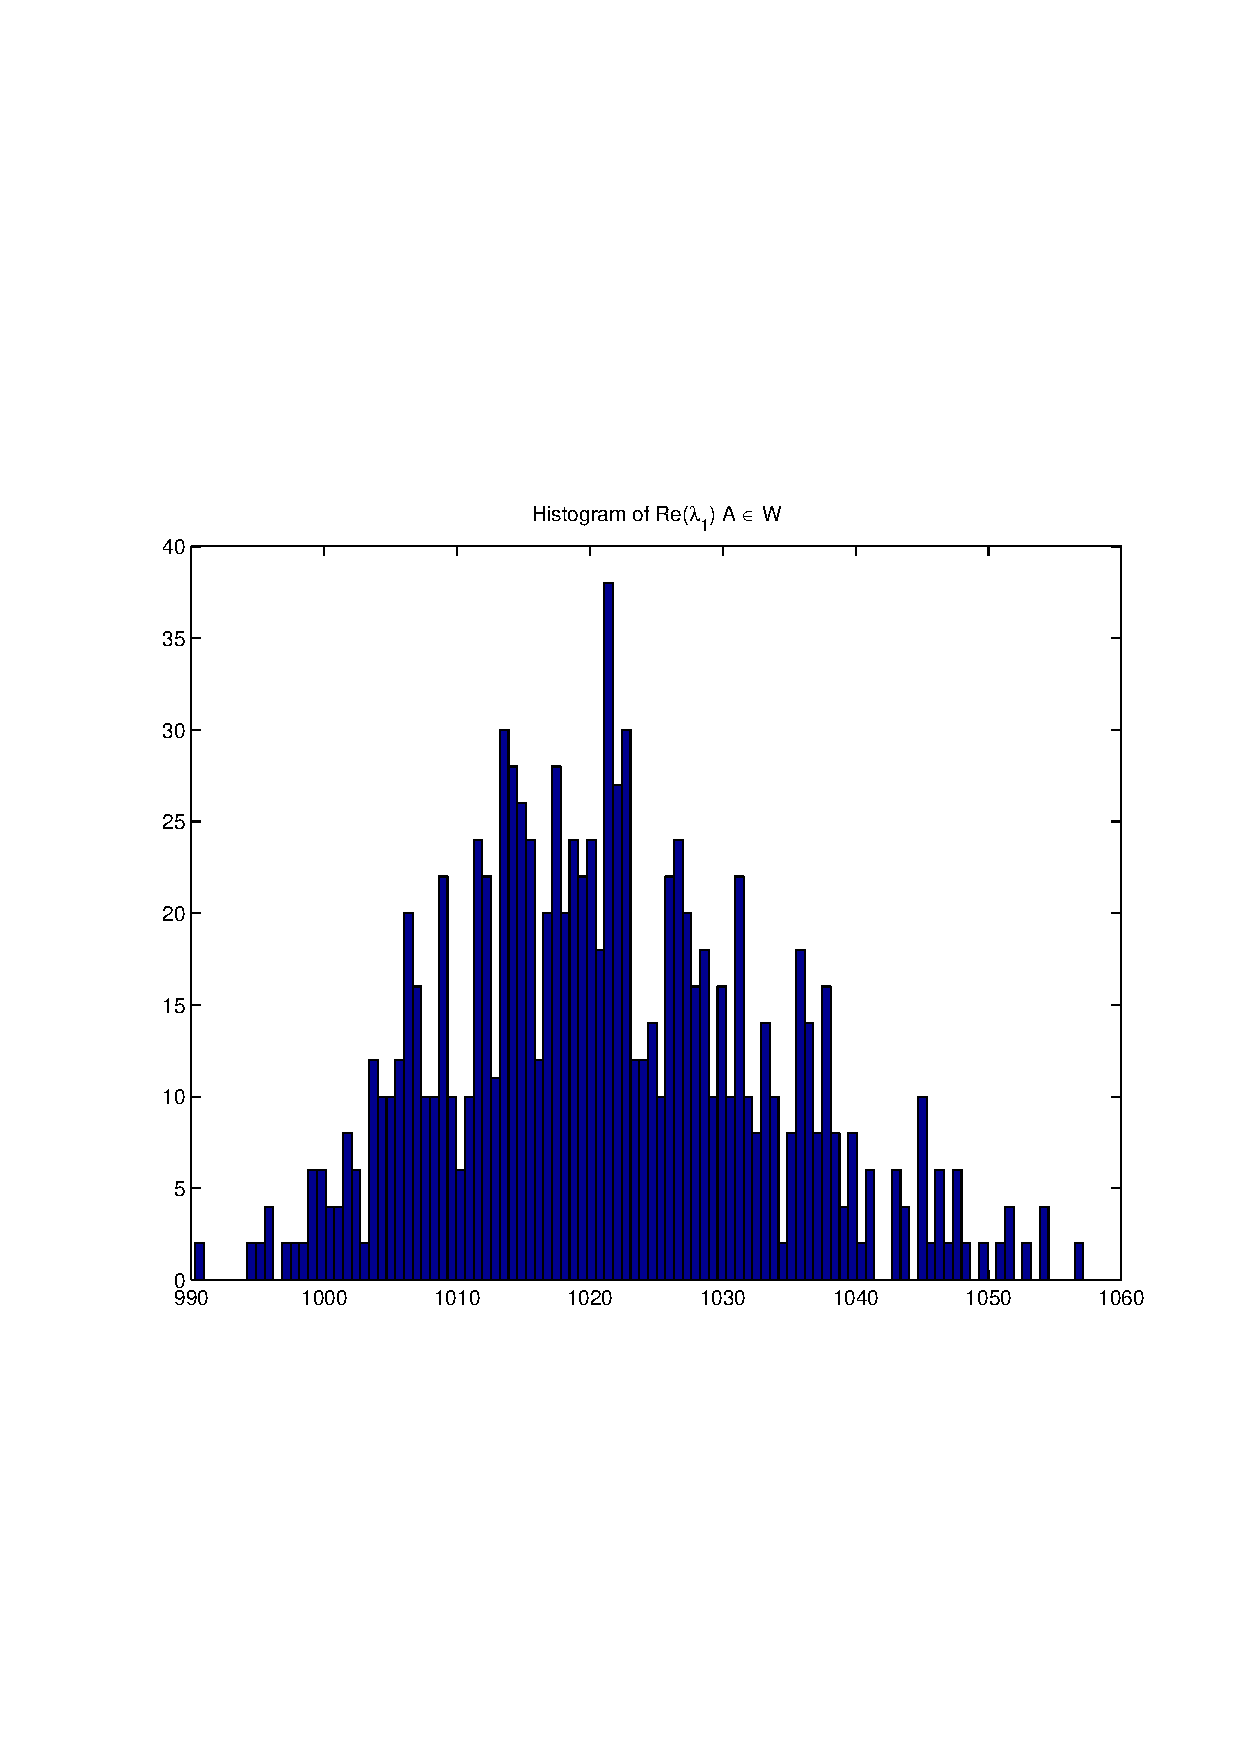
\includegraphics[width=10.0cm,height=10.0cm]{Re_TraceyWidom.pdf}

\includegraphics[width=10.0cm,height=10.0cm]{Im_TraceyWidom.pdf}

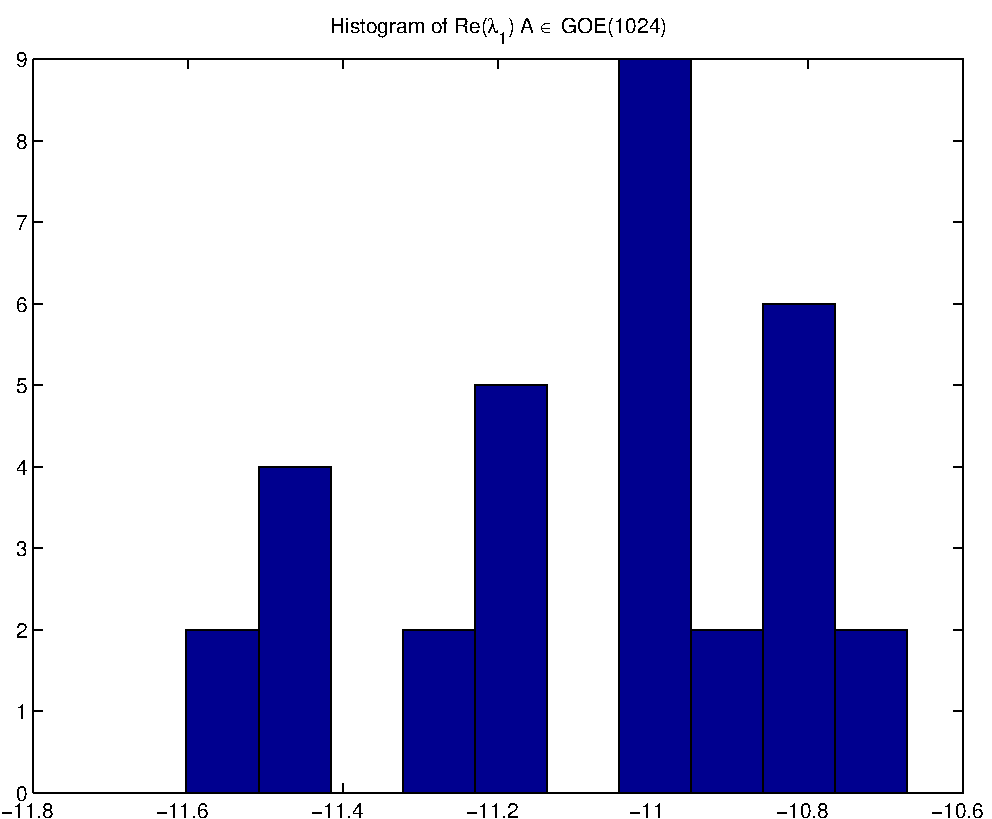
\includegraphics[width=10.0cm,height=10.0cm]{Re_Winger.pdf}

\includegraphics[width=10.0cm,height=10.0cm]{Im_Winger.pdf}

QueryPerformanceCounter  =  +5.239
\subsubsection{Approximate Winger Distribution}
\subsubsection{Verfy Winger Law.}
Let $M_n = [X_{ij} ]$ a symmetric n x n matrix with Random entries such that $X_{i,j} = X_{j,i}$, 		  and $X_{i,j}$ are iid $orall i < j,$ and $Xjj$ are iid $orall j  :  ; E[X^2_{ij} ] = 1, & E[X_{ij}] = 0$ 		  and that all moments exists for each of the entries.  		  The eigenvector of this random matrix; $ lambda_1 leq ... leq lambda_n$ depends continuously on $Mn$.
Dimension $n = +512$

\includegraphics[width=10.0cm,height=10.0cm]{Re_lambda_n.pdf}

\includegraphics[width=10.0cm,height=10.0cm]{Im_lambda_n.pdf}

QueryPerformanceCounter  =  +2.728
\subsubsection{Matrix Exponential }
$SPD Matrix = \left(
\begin{array}{
cccccccc}
+10.539 & -0.499 & -0.010 & +0.368 & +0.465 & -0.492 & -0.126 & +0.437 \\
-0.499 & +7.286 & +0.365 & -0.481 & -0.337 & -0.466 & +0.279 & +0.056 \\
-0.010 & +0.365 & +6.705 & -0.205 & +0.467 & +0.131 & +0.077 & -0.089 \\
+0.368 & -0.481 & -0.205 & +6.496 & -0.402 & -0.209 & +0.043 & -0.041 \\
+0.465 & -0.337 & +0.467 & -0.402 & +4.578 & +0.272 & +0.289 & -0.285 \\
-0.492 & -0.466 & +0.131 & -0.209 & +0.272 & +8.181 & +0.343 & -0.244 \\
-0.126 & +0.279 & +0.077 & +0.043 & +0.289 & +0.343 & +5.938 & -0.212 \\
+0.437 & +0.056 & -0.089 & -0.041 & -0.285 & -0.244 & -0.212 & +9.691 \\
\end{array}
\right)$ \newline 

$SPD Eigs = \left(
\begin{array}{
cccccccc}
(+10.93611,+0.00000) & (+9.60778,+0.00000) & (+4.23666,+0.00000) & (+8.36911,+0.00000) & (+7.56229,+0.00000) & (+5.82791,+0.00000) & (+6.54198,+0.00000) & (+6.33139,+0.00000) \\
\end{array}
\right)$ \newline 

$exp(SPD) = \left(
\begin{array}{
cccccccc}
+47863.969 & -6460.093 & -1078.770 & +4706.958 & +2535.224 & -8475.398 & -2406.368 & +12977.552 \\
-6460.093 & +2780.574 & +516.920 & -1069.918 & -548.083 & -109.707 & +386.466 & -807.216 \\
-1078.770 & +516.920 & +1015.281 & -385.755 & +176.069 & +458.541 & +212.284 & -859.022 \\
+4706.958 & -1069.918 & -385.755 & +1267.210 & +111.181 & -1018.272 & -287.809 & +1036.628 \\
+2535.224 & -548.083 & +176.069 & +111.181 & +413.265 & +135.193 & +45.490 & -502.411 \\
-8475.398 & -109.707 & +458.541 & -1018.272 & +135.193 & +5613.026 & +968.003 & -4270.737 \\
-2406.368 & +386.466 & +212.284 & -287.809 & +45.490 & +968.003 & +632.432 & -1645.725 \\
+12977.552 & -807.216 & -859.022 & +1036.628 & -502.411 & -4270.737 & -1645.725 & +19362.944 \\
\end{array}
\right)$ \newline 

$exp(SPD) eigs = \left(
\begin{array}{
cccccccc}
(+56168.17045,+0.00000) & (+14880.07985,+0.00000) & (+4311.77579,+0.00000) & (+1924.25027,+0.00000) & (+69.17669,+0.00000) & (+339.64809,+0.00000) & (+693.66208,+0.00000) & (+561.93669,+0.00000) \\
\end{array}
\right)$ \newline 

$log(exp(SPD) eigs)  = \left(
\begin{array}{
cccccccc}
(+10.93611,+0.00000) & (+9.60778,+0.00000) & (+8.36911,+0.00000) & (+7.56229,+0.00000) & (+4.23666,+0.00000) & (+5.82791,+0.00000) & (+6.54198,+0.00000) & (+6.33139,+0.00000) \\
\end{array}
\right)$ \newline 

$exp(Id) = \left(
\begin{array}{
cccccccc}
+2.718 & +0.000 & +0.000 & +0.000 & +0.000 & +0.000 & +0.000 & +0.000 \\
+0.000 & +2.718 & +0.000 & +0.000 & +0.000 & +0.000 & +0.000 & +0.000 \\
+0.000 & +0.000 & +2.718 & +0.000 & +0.000 & +0.000 & +0.000 & +0.000 \\
+0.000 & +0.000 & +0.000 & +2.718 & +0.000 & +0.000 & +0.000 & +0.000 \\
+0.000 & +0.000 & +0.000 & +0.000 & +2.718 & +0.000 & +0.000 & +0.000 \\
+0.000 & +0.000 & +0.000 & +0.000 & +0.000 & +2.718 & +0.000 & +0.000 \\
+0.000 & +0.000 & +0.000 & +0.000 & +0.000 & +0.000 & +2.718 & +0.000 \\
+0.000 & +0.000 & +0.000 & +0.000 & +0.000 & +0.000 & +0.000 & +2.718 \\
\end{array}
\right)$ \newline 

$exp(Id) eigs = \left(
\begin{array}{
cccccccc}
(+2.71828,+0.00000) & (+2.71828,+0.00000) & (+2.71828,+0.00000) & (+2.71828,+0.00000) & (+2.71828,+0.00000) & (+2.71828,+0.00000) & (+2.71828,+0.00000) & (+2.71828,+0.00000) \\
\end{array}
\right)$ \newline 

$log(exp(Id) eigs)  = \left(
\begin{array}{
cccccccc}
(+1.00000,+0.00000) & (+1.00000,+0.00000) & (+1.00000,+0.00000) & (+1.00000,+0.00000) & (+1.00000,+0.00000) & (+1.00000,+0.00000) & (+1.00000,+0.00000) & (+1.00000,+0.00000) \\
\end{array}
\right)$ \newline 

For $n  \in  \dblz [16,128)$ we calculate  $|( SPD(n) Eigs - log(exp(SPD(n)) eigs)|_{l^2}$

$|( SPD(n) Eigs - log(exp(SPD(n)) eigs)|_{l^2} = \left(
\begin{array}{
cccccccccccccccccccccccccccccccccccccccccccccccccccccccccccccccccccccccccccccccccccccccccccccccccccccccccccccccc}
(+5.36543,+0.00000) & (+5.36543,+0.00000) & (+5.36543,+0.00000) & (+5.36543,+0.00000) & (+5.36543,+0.00000) & (+5.36543,+0.00000) & (+5.36543,+0.00000) & (+5.36543,+0.00000) & (+5.36543,+0.00000) & (+5.36543,+0.00000) & (+5.36543,+0.00000) & (+5.36543,+0.00000) & (+5.36543,+0.00000) & (+5.36543,+0.00000) & (+5.36543,+0.00000) & (+5.36543,+0.00000) & (+5.36543,+0.00000) & (+5.36543,+0.00000) & (+5.36543,+0.00000) & (+5.36543,+0.00000) & (+5.36543,+0.00000) & (+5.36543,+0.00000) & (+5.36543,+0.00000) & (+5.36543,+0.00000) & (+5.36543,+0.00000) & (+5.36543,+0.00000) & (+5.36543,+0.00000) & (+5.36543,+0.00000) & (+5.36543,+0.00000) & (+5.36543,+0.00000) & (+5.36543,+0.00000) & (+5.36543,+0.00000) & (+5.36543,+0.00000) & (+5.36543,+0.00000) & (+5.36543,+0.00000) & (+5.36543,+0.00000) & (+5.36543,+0.00000) & (+5.36543,+0.00000) & (+5.36543,+0.00000) & (+5.36543,+0.00000) & (+5.36543,+0.00000) & (+5.36543,+0.00000) & (+5.36543,+0.00000) & (+5.36543,+0.00000) & (+5.36543,+0.00000) & (+5.36543,+0.00000) & (+5.36543,+0.00000) & (+5.36543,+0.00000) & (+0.00000,+0.00000) & (+0.00000,+0.00000) & (+0.00000,+0.00000) & (+0.00000,+0.00000) & (+0.00000,+0.00000) & (+0.00000,+0.00000) & (+0.00000,+0.00000) & (+0.00000,+0.00000) & (+0.00000,+0.00000) & (+0.00000,+0.00000) & (+0.00000,+0.00000) & (+0.00000,+0.00000) & (+0.00000,+0.00000) & (+0.00000,+0.00000) & (+0.00000,+0.00000) & (+0.00000,+0.00000) & (+0.00000,+0.00000) & (+0.00000,+0.00000) & (+0.00000,+0.00000) & (+0.00000,+0.00000) & (+0.00000,+0.00000) & (+0.00000,+0.00000) & (+0.00000,+0.00000) & (+0.00000,+0.00000) & (+0.00000,+0.00000) & (+0.00000,+0.00000) & (+0.00000,+0.00000) & (+0.00000,+0.00000) & (+0.00000,+0.00000) & (+0.00000,+0.00000) & (+0.00000,+0.00000) & (+0.00000,+0.00000) & (+0.00000,+0.00000) & (+0.00000,+0.00000) & (+0.00000,+0.00000) & (+0.00000,+0.00000) & (+0.00000,+0.00000) & (+0.00000,+0.00000) & (+0.00000,+0.00000) & (+0.00000,+0.00000) & (+0.00000,+0.00000) & (+0.00000,+0.00000) & (+0.00000,+0.00000) & (+0.00000,+0.00000) & (+0.00000,+0.00000) & (+0.00000,+0.00000) & (+0.00000,+0.00000) & (+0.00000,+0.00000) & (+0.00000,+0.00000) & (+0.00000,+0.00000) & (+0.00000,+0.00000) & (+0.00000,+0.00000) & (+0.00000,+0.00000) & (+0.00000,+0.00000) & (+0.00000,+0.00000) & (+0.00000,+0.00000) & (+0.00000,+0.00000) & (+0.00000,+0.00000) & (+0.00000,+0.00000) & (+0.00000,+0.00000) & (+0.00000,+0.00000) & (+0.00000,+0.00000) & (+0.00000,+0.00000) & (+0.00000,+0.00000) \\
\end{array}
\right)$ \newline 

QueryPerformanceCounter  =  +0.00952
The sample size generated for this run is 100000.

\newpage
uniform \begin{tabular}{|c|c|c|c|}  mean & variance & skewness & kurtosis \\  \hline
$\mu_1 = +0.50030$ & $\mu_2 = +0.08353$ & $\mu_3 = +0.00339$ & $\mu_4 =+1.80113$ \\
\end{tabular}

\includegraphics[width=5cm,height=5cm]{uniform.pdf}

cauchy \begin{tabular}{|c|c|c|c|}  mean & variance & skewness & kurtosis \\  \hline
$\mu_1 = +0.44288$ & $\mu_2 = +0.05341$ & $\mu_3 = +0.63935$ & $\mu_4 =+3.28094$ \\
\end{tabular}

\includegraphics[width=5cm,height=5cm]{cauchy.pdf}

exponential \begin{tabular}{|c|c|c|c|}  mean & variance & skewness & kurtosis \\  \hline
$\mu_1 = +1.99647$ & $\mu_2 = +3.99339$ & $\mu_3 = +2.03097$ & $\mu_4 =+9.30842$ \\
\end{tabular}

\includegraphics[width=5cm,height=5cm]{exponential.pdf}

\newpage
gamma \begin{tabular}{|c|c|c|c|}  mean & variance & skewness & kurtosis \\  \hline
$\mu_1 = +1.90699$ & $\mu_2 = +1.92200$ & $\mu_3 = +1.43217$ & $\mu_4 =+6.00417$ \\
\end{tabular}

\includegraphics[width=5cm,height=5cm]{gamma.pdf}

GIG \begin{tabular}{|c|c|c|c|}  mean & variance & skewness & kurtosis \\  \hline
$\mu_1 = +0.80701$ & $\mu_2 = +11.65676$ & $\mu_3 = +15.50173$ & $\mu_4 =+322.28720$ \\
\end{tabular}

\includegraphics[width=5cm,height=5cm]{GIG.pdf}

normal-box-muller \begin{tabular}{|c|c|c|c|}  mean & variance & skewness & kurtosis \\  \hline
$\mu_1 = +0.00208$ & $\mu_2 = +0.99953$ & $\mu_3 = -0.00837$ & $\mu_4 =+3.00580$ \\
\end{tabular}

\includegraphics[width=5cm,height=5cm]{normal-box-muller.pdf}

\newpage
normal-inverse-approximation \begin{tabular}{|c|c|c|c|}  mean & variance & skewness & kurtosis \\  \hline
$\mu_1 = +0.00230$ & $\mu_2 = +1.00486$ & $\mu_3 = +0.01163$ & $\mu_4 =+2.99254$ \\
\end{tabular}

\includegraphics[width=5cm,height=5cm]{normal-inverse-approximation.pdf}

pareto \begin{tabular}{|c|c|c|c|}  mean & variance & skewness & kurtosis \\  \hline
$\mu_1 = +3184578.26493$ & $\mu_2 = +888468246174112900.00000$ & $\mu_3 = +315.36997$ & $\mu_4 =+99629.09819$ \\
\end{tabular}

\includegraphics[width=5cm,height=5cm]{pareto.pdf}

poisson \begin{tabular}{|c|c|c|c|}  mean & variance & skewness & kurtosis \\  \hline
$\mu_1 = +1.10640$ & $\mu_2 = +0.13092$ & $\mu_3 = +3.88950$ & $\mu_4 =+20.71460$ \\
\end{tabular}

\includegraphics[width=5cm,height=5cm]{poisson.pdf}

\newpage
beta \begin{tabular}{|c|c|c|c|}  mean & variance & skewness & kurtosis \\  \hline
$\mu_1 = +0.33334$ & $\mu_2 = +0.12690$ & $\mu_3 = +0.68168$ & $\mu_4 =+1.91290$ \\
\end{tabular}

\includegraphics[width=5cm,height=5cm]{beta.pdf}

QueryPerformanceCounter  =  +10.99767
\subsubsection{Multiclass Support Vector Machine }
\begin{itemize}
\item Number or training points = 1024
\item Feature dimension = 3
\item Number or classes = 3
\end{itemize}
{The mean vectors of the 3 classes}

$\mu_1 = \left(
\begin{array}{
ccc}
+1.90000 & +0.10000 & +0.10000 \\
\end{array}
\right)$ \newline 

$\mu_2 = \left(
\begin{array}{
ccc}
+0.10000 & +1.90000 & +0.10000 \\
\end{array}
\right)$ \newline 

$\mu_3 = \left(
\begin{array}{
ccc}
+0.00000 & +0.00000 & +1.90000 \\
\end{array}
\right)$ \newline 

A random SPD covairance matrix is generated for each of the classes.\newline

$\rho_1 = \left(
\begin{array}{
ccc}
+2.441 & -0.047 & -0.469 \\
-0.047 & +3.169 & -0.024 \\
-0.469 & -0.024 & +4.350 \\
\end{array}
\right)$ \newline 

$\rho_2 = \left(
\begin{array}{
ccc}
+2.923 & +0.025 & +0.150 \\
+0.025 & +4.215 & -0.043 \\
+0.150 & -0.043 & +4.080 \\
\end{array}
\right)$ \newline 

$\rho_3 = \left(
\begin{array}{
ccc}
+4.249 & +0.094 & -0.265 \\
+0.094 & +3.193 & +0.099 \\
-0.265 & +0.099 & +4.012 \\
\end{array}
\right)$ \newline 

Verify $L_1$ condition number of covariance. The diagonal entries of the matrix have the form $(0.5 + U(0,1) )*dim(Dom(Cov))$
The lower-diagonal entries take the form $U(0,1) - 0.5$. 
The $L_1$ condition numbers are :
\begin{itemize}
\item +2.277
\item +1.532
\item +1.518
\end{itemize}
\includegraphics[width=10.0cm,height=10.0cm]{rv1_corr.pdf}

\includegraphics[width=10.0cm,height=10.0cm]{rv2_corr.pdf}

\includegraphics[width=10.0cm,height=10.0cm]{rv3_corr.pdf}

\includegraphics[width=10.0cm,height=10.0cm]{trainingPoints.pdf}

These are the SVM parameters - the RBF kernel is used\begin{itemize}
\item allOutlierFraction=0.05
\item mixingCoeff=0.3
\item smoThresh=1.0/10000.0
\item sigma=1
\end{itemize}
\includegraphics[width=10.0cm,height=10.0cm]{testPoints.pdf}

The marginal sample moments (mean var skew kurtosis) for training points.\newline
\begin{tabular}{ c |  c  c  c  c}
Feature & $\mu_1$ & $\mu_2$ & $\mu_3$ & $\mu_4$ \\
0 & +0.668 & +1.407 & +0.052& +2.299 \\
\hline
1 & +0.707 & +1.377 & +0.436& +2.580 \\
\hline
2 & +0.701 & +1.517 & +0.225& +2.572 \\
\hline
\end{tabular}
\newline
The marginal sample moments (mean var skew kurtosis) for test points.\newline
\begin{tabular}{ c | c  c  c  c}
Feature & $\mu_1$ & $\mu_2$ & $\mu_3$ & $\mu_4$ \\
0 & +0.677 & +1.297 & +0.181& +2.370\\
\hline
1 & +0.670 & +1.371 & +0.470& +2.590\\
\hline
2 & +0.726 & +1.442 & +0.207& +2.452\\
\hline
\end{tabular}\newline
\includegraphics[width=10.0cm,height=10.0cm]{classDiffs.pdf}

The error rate for this run is +0.311\newline
QueryPerformanceCounter  =  +5.930
\subsubsection{Semidefinite Programming SDPA}
QueryPerformanceCounter  =  +0.005
\end{document}
